\documentclass[UTF8,a4paper,zihao=-4,fontset=fandol]{ctexart}

\usepackage{geometry}
\geometry{top=2.54cm,bottom=2.54cm,left=3.17cm,right=3.17cm}
\usepackage{graphicx}
\usepackage{float}
\usepackage{booktabs}
\usepackage{array}
\usepackage{amsmath,amssymb}
\usepackage{longtable}
\usepackage{caption}
\usepackage{subcaption}
\usepackage{hyperref}
\usepackage{setspace}
\usepackage{indentfirst}

\graphicspath{{paper/figures/}{figures/}}
\hypersetup{colorlinks=true,linkcolor=black,citecolor=black,urlcolor=black}
\captionsetup{font=small,labelsep=quad}
\setlength{\parindent}{2em}
\setlength{\parskip}{0pt}
\setstretch{1.45}

\newif\ifanonymous
\ifdefined\ANONYMOUS
  \anonymoustrue
\else
  \anonymousfalse
\fi

\title{基于高分辨率海温资料的南海增暖及海洋热浪风险统计建模研究}
\author{}
\date{}

\begin{document}

\ifanonymous\else
\begin{titlepage}
  \centering
  \vspace*{0.5cm}
  {\heiti\zihao{3} 作品编号：TJJM2026XXXXXXX\par}
  \vspace{2.2cm}
  {\songti\zihao{1} 2026年（第十二届）全国大学生统计建模大赛\par}
  \vspace{0.7cm}
  {\songti\zihao{1} 参\ 赛\ 作\ 品\par}
  \vspace{2.3cm}
  {\fangsong\zihao{2} 参赛学校：华南农业大学\par}
  \vspace{0.8cm}
  {\fangsong\zihao{2} 论文题目：\par}
  \vspace{0.3cm}
  {\songti\zihao{3} 基于高分辨率海温资料的南海增暖及海洋热浪风险统计建模研究\par}
  \vspace{0.8cm}
  {\fangsong\zihao{2} 参赛队员：待填写\par}
  \vspace{0.8cm}
  {\fangsong\zihao{2} 指导老师：（暂时不填）\par}
  \vfill
\end{titlepage}
\fi

\begin{center}
{\songti\zihao{3} 基于高分辨率海温资料的南海增暖及海洋热浪风险统计建模研究}
\end{center}

\section*{摘要}
南海处于西太平洋暖池西缘和东亚季风影响区，海表温度变化同时关系到海气相互作用、近海生态系统和海洋资源安全。仅使用平均海温趋势难以刻画持续性高温暴露，仅识别极端事件又容易忽略长期增暖背景。为统一量化南海平均态增暖与极端热风险，本文基于 1991--2021 年 OSTIA 日尺度高分辨率海表温度资料，裁剪得到 $5^{\circ}$S--$25^{\circ}$N、$100^{\circ}$E--$125^{\circ}$E 的南海网格数据，构建“平均态增暖测度--海洋热浪事件识别--空间分区比较--稳健性检验--驱动因子解释”的统计建模框架。具体方法包括面积加权区域平均、月气候态距平、线性趋势估计、Theil-Sen 斜率与 Kendall 单调趋势诊断、Hobday 海洋热浪事件识别、85\%/90\%/95\% 阈值敏感性检验、分区统计、相对综合海洋热风险指数以及标准化多元回归模型。

结果表明，1991--2021 年南海区域平均 SST 和 SSTA 均呈显著上升趋势，线性趋势分别为 $0.191\,^{\circ}\mathrm{C}/10a$ 和 $0.174\,^{\circ}\mathrm{C}/10a$；非参数检验中，SSTA 的 Theil-Sen 趋势为 $0.179\,^{\circ}\mathrm{C}/10a$，Kendall $\tau=0.351$ 且 $p<0.001$，说明平均态增暖结论具有稳健性。同期海洋热浪风险显著增强，区域平均 MHW 频次、总天数和累计强度分别增加 $1.308$ 次/10年、$13.381$ 天/10年和 $15.176\,^{\circ}\mathrm{C}\cdot\mathrm{d}/10a$；在 85\%、90\% 和 95\% 三组阈值下，总天数和累计强度趋势均保持正向。分区结果显示，北部陆架 MHW 总天数趋势达到 $14.547$ 天/10年，综合热风险指数均值为 0.574，高风险格点占比为 16.6\%，是本文识别的重点关注区域。驱动因子分析表明，风速距平是最稳定的解释变量，其对月尺度 SSTA 和年度 MHW 总天数的标准化回归系数分别为 $-0.363$ 和 $-0.558$。本文的主要创新在于将高分辨率日尺度海温资料、极端事件识别、稳健趋势检验、分区风险综合和解释型统计模型统一到可复现框架中，为南海海洋热风险监测和区域适应性管理提供了量化依据。

\noindent\textbf{关键词：} 南海；海表温度；海洋热浪；稳健趋势检验；综合风险指数

\newpage
\tableofcontents
\newpage
\listoftables
\listoffigures
\newpage

\section{引言}

\subsection{研究背景}
海表温度（Sea Surface Temperature, SST）是描述海洋热状态、海气热量交换和海洋生态环境变化的基础变量。南海位于西太平洋暖池西缘，受东亚季风、低纬海气相互作用、黑潮入侵和陆架环流共同影响，具有明显的季节循环和空间差异。南海同时承载珊瑚礁、渔业资源、近岸养殖和海洋保护区等多类生态与经济功能，因此其海表热环境变化具有明确的现实意义。

全球变暖背景下，海洋热风险并不只表现为年均或月均温度升高。对于珊瑚礁白化、海草床退化、养殖风险和近海生态胁迫而言，持续多日的异常高温暴露往往比单日最高温或年平均温度更直接。海洋热浪（Marine Heatwave, MHW）正是针对这种持续性异常高温过程提出的统计事件定义。Hobday 等\cite{hobday2016mhw}提出的逐日分位阈值方法，使不同海域的海洋极端热事件具有可比性，也为统计建模提供了可复现的事件识别标准。

已有研究通常从四类路径分析海洋热环境变化：一是利用卫星融合或再分析资料评估海温长期趋势；二是按统一阈值识别海洋热浪事件并比较频次、持续时间和强度；三是将 ENSO、IOD、风场和热通量等因子作为海温异常的解释变量；四是面向生态系统讨论高温暴露的潜在影响\cite{oliver2018longer,holbrook2019mhw,smale2019mhw}。这些工作为本文提供了方法基础，但在统计建模竞赛语境下，若只给出单一趋势值或单一预测模型，仍不足以形成完整论证。一个完整的统计建模方案应当同时回答：研究对象如何被量化，模型结果是否稳健，空间差异如何表达，结论能否服务实际管理。

基于上述认识，本文不将主线设定为未来预测，而是把南海海表热环境变化抽象为两个相互联系的统计对象：一是平均态海表温度和距平的长期变化，二是以持续高温事件为核心的极端热风险。围绕这两个对象，本文提出五个研究问题：1991--2021 年南海是否存在显著增暖；增暖是否具有空间异质性；海洋热浪风险是否在频次、暴露时长和累计强度上同步增强；主要结论是否对趋势方法和阈值选择稳健；气候指数和局地风场能否解释部分年际波动。

\subsection{研究思路与创新点}
本文的技术路线见图 1。研究首先对 OSTIA 日尺度 SST 资料进行南海区域裁剪和质量检查；其次基于月气候态构造 SSTA 并估计区域平均和格点趋势；再次按照逐日分位阈值识别海洋热浪事件，聚合形成年度风险指标；随后开展分区统计、稳健性检验和综合热风险指数构建；最后引入气候指数和 10 m 风场资料建立解释型统计模型。

\begin{figure}[H]
\centering
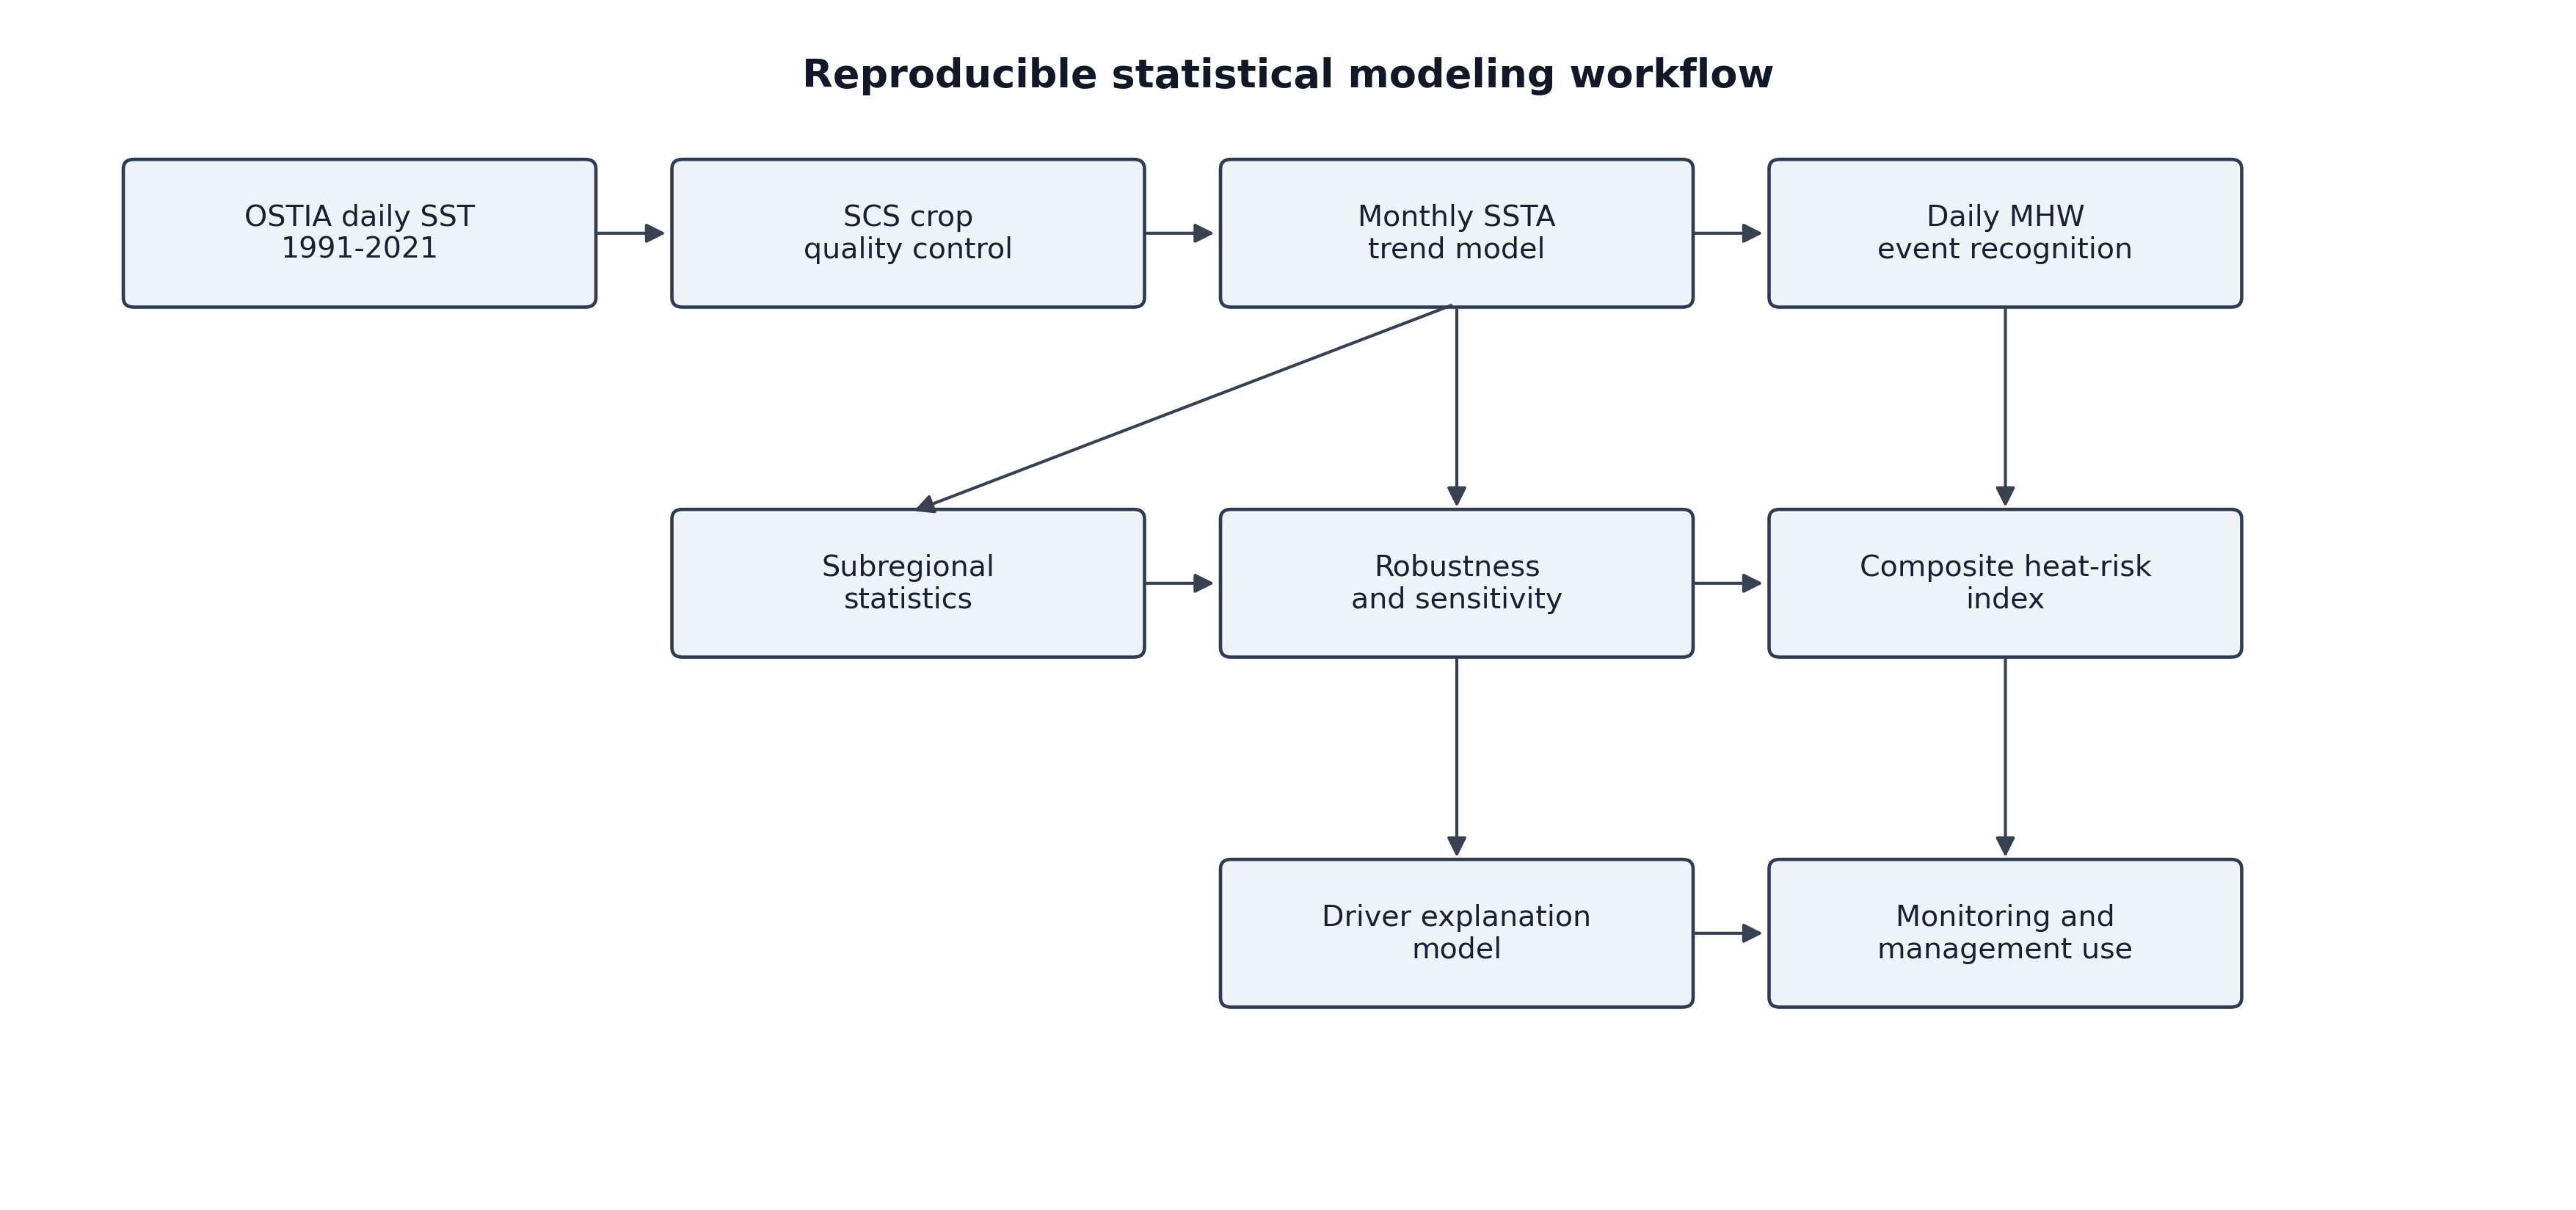
\includegraphics[width=\textwidth]{workflow_diagram.png}
\caption{研究技术路线}
\end{figure}

本文的创新主要体现在四个方面。第一，数据尺度统一：以日尺度 OSTIA 资料为基础，同时支撑月尺度平均态增暖分析和日尺度极端事件识别，避免不同数据源混用带来的空间和时间口径差异。第二，指标体系完整：将 SST、SSTA、MHW 频次、总天数、强度、分区趋势和综合风险指数纳入同一框架，使平均态、极端事件和空间优先区相互补充。第三，模型检验充分：在普通最小二乘趋势之外加入 Theil-Sen 斜率、Kendall 单调趋势诊断和 MHW 阈值敏感性检验，减少结论对单一模型设定的依赖。第四，结果可解释可应用：通过标准化回归比较风场和气候指数的解释强度，并将综合热风险指数转化为区域监测优先级。

\section{研究区、数据来源与质量控制}

\subsection{研究区与数据来源}
本文研究区设定为 $5^{\circ}$S--$25^{\circ}$N、$100^{\circ}$E--$125^{\circ}$E，覆盖南海主体海域、北部陆架、中部海盆、南部岛礁区以及低纬邻近海域。该范围能够较完整地反映南海从近岸陆架到深海盆地、从热带低纬到副热带边缘的热环境梯度。所有区域平均和分区平均均在原始规则经纬度网格上计算，并使用 $\cos(\varphi)$ 作为纬向面积权重。

核心 SST 数据来自 OSTIA（Operational Sea Surface Temperature and Sea Ice Analysis）高分辨率海温分析产品。OSTIA 是公开的全球 L4 SST 资料，通过多源卫星观测、现场观测和最优插值方法生成无缝海温场\cite{donlon2012ostia,copernicus2026ostia}。本文使用 1991--2021 年日尺度 SST，并由日尺度资料聚合得到月尺度 SST。解释变量包括 NOAA/PSL 提供的 Niño 3.4、PDO、DMI 和 SOI 月度气候指数，以及 NCEP/NCAR Reanalysis 1 的 10 m 纬向和经向风场\cite{kalnay1996ncep,noaapsl2026indices}。数据基本信息如表 1 所示。

\begin{table}[H]
\centering
\caption{研究数据基本信息}
\resizebox{\textwidth}{!}{\begin{tabular}{lc}
\hline
项目 & 说明 \\
\hline
研究区范围 & $5^{\circ}$S--$25^{\circ}$N, $100^{\circ}$E--$125^{\circ}$E \\
日尺度 SST 栅格 & 11261 天 $\times$ 600 纬度 $\times$ 500 经度 \\
月尺度 SST 栅格 & 372 月 $\times$ 600 纬度 $\times$ 500 经度 \\
气候态基准期 & 1991--2020 年 \\
缺失日历月份 & 2014-07、2015-12 \\
全海域无效月份 & 2015-11 \\
有效海洋格点数 & 193341 \\
\hline
\end{tabular}
}
\end{table}

\subsection{数据预处理与缺测处理}
原始 SST 数据经空间裁剪、单位转换、海洋掩膜和时间聚合后，形成日尺度和月尺度两个分析产品。月尺度产品用于气候态、距平和长期趋势估计；日尺度产品用于逐格点海洋热浪阈值计算和事件识别。面积平均时仅使用海洋格点，陆地格点权重设为 0。

资料检查发现，本地 OSTIA/Copernicus 源文件存在三个不可用月份：2014 年 7 月和 2015 年 12 月缺失全部日历日，2015 年 11 月虽有日记录但研究区海洋格点 SST 全部为缺失值。考虑到这些缺测集中于完整月份，直接插值可能人为制造或削弱连续高温事件，本文采取保守策略：月尺度趋势、相关和回归计算排除缺失月份；日尺度 MHW 识别中，缺失日和全无效日不计入有效日数，并打断连续事件。该处理方式使模型不把无观测信息误判为无风险，也为后续缺测敏感性检验提供了明确口径。

\subsection{分区设定}
为避免只用全南海平均值掩盖空间差异，本文根据纬度、陆架海盆结构和近岸外海差异划分五个统计分区：北部陆架（$15^{\circ}$N--$25^{\circ}$N，$105^{\circ}$E--$122^{\circ}$E）、中部海盆（$8^{\circ}$N--$18^{\circ}$N，$110^{\circ}$E--$118^{\circ}$E）、南部南海（$5^{\circ}$S--$8^{\circ}$N，$105^{\circ}$E--$118^{\circ}$E）、西部近岸（$5^{\circ}$N--$22^{\circ}$N，$100^{\circ}$E--$110^{\circ}$E）和东部外海（$5^{\circ}$N--$22^{\circ}$N，$110^{\circ}$E--$125^{\circ}$E）。分区边界并非行政区划，而是用于比较不同海洋热环境背景下统计指标的相对变化。

\section{指标体系与统计建模方法}

\subsection{面积加权平均与海温距平}
设 $T_{tij}$ 表示时间 $t$、纬度 $i$、经度 $j$ 的 SST，$M_{ij}$ 为海洋掩膜，纬度为 $\varphi_i$。区域面积加权平均定义为
\begin{equation}
\bar{T}_{t}=\frac{\sum_{i,j}T_{tij}M_{ij}\cos\varphi_i}{\sum_{i,j}M_{ij}\cos\varphi_i}.
\end{equation}
该权重近似反映规则经纬度网格随纬度变化的面积差异，使区域平均不被高纬较小面积格点过度影响。月尺度气候态以 1991--2020 年为基准期，对每个自然月分别计算多年平均，SSTA 定义为
\begin{equation}
A_t=\bar{T}_t-\overline{T}_{m(t)}^{\,clim},
\end{equation}
其中 $m(t)$ 表示月份。距平指标用于消除季节循环，使长期趋势和年际波动具有可比性。

\subsection{趋势估计与稳健性检验}
对区域平均序列和空间格点序列，首先建立线性趋势模型：
\begin{equation}
y_t=\alpha+\beta x_t+\varepsilon_t,
\end{equation}
其中 $x_t$ 为距起始时刻的年份数，$\beta$ 表示单位年份变化率。本文将 $\beta$ 乘以 10，报告为每 10 年变化量。线性趋势便于解释长期平均变化速率，也便于与回归模型中的年际变化分析保持一致。

为检验结论是否依赖普通最小二乘的分布假设，本文同时计算 Theil-Sen 斜率和 Kendall 单调趋势诊断。Theil-Sen 斜率取所有两点斜率的中位数：
\begin{equation}
\hat{\beta}_{TS}=\mathrm{median}_{i<j}\left(\frac{y_j-y_i}{x_j-x_i}\right).
\end{equation}
该方法对异常年份更稳健。Kendall $\tau$ 用于衡量时间与指标之间的单调一致性，若 OLS、Theil-Sen 和 Kendall 检验方向一致，则认为趋势结论具有较强稳健性。

\subsection{海洋热浪事件识别模型}
本文采用 Hobday 等\cite{hobday2016mhw}提出的海洋热浪定义。对每个海洋格点，以 1991--2020 年为基准期，保留 366 日历日，并对每个日序使用前后共 11 日滑动窗口计算逐日气候态均值 $C_d$ 和分位阈值 $Q_{p,d}$。主模型使用 90\% 分位阈值：
\begin{equation}
T_t>Q_{0.9,d(t)}.
\end{equation}
若上述条件连续满足不少于 5 个有效日，则识别为一次 MHW 事件。事件强度定义为 $T_t-C_{d(t)}$。年度 MHW 指标包括频次、总天数、平均持续时间、最长持续时间、最大强度和累计强度。本文进一步使用 85\% 和 95\% 阈值重新识别事件，以检验结果是否依赖单一阈值。

\subsection{综合海洋热风险指数}
为将多个风险维度转化为空间优先级，本文构建相对综合海洋热风险指数（Heat Risk Index, HRI）。HRI 由四个分量等权合成：SSTA 趋势、MHW 总天数多年平均、MHW 总天数趋势和 MHW 累计强度趋势。对每个分量在有效海洋格点上做极差标准化：
\begin{equation}
Z_k(i,j)=\frac{X_k(i,j)-\min(X_k)}{\max(X_k)-\min(X_k)}.
\end{equation}
综合指数定义为
\begin{equation}
HRI(i,j)=\frac{1}{4}\sum_{k=1}^{4}Z_k(i,j).
\end{equation}
当某一分量无有效取值范围时，剔除该分量并对剩余权重重新归一化。HRI 是相对风险优先级指标，并不表示绝对生态损失概率。本文将 $HRI<0.33$ 定义为低风险，$0.33\leq HRI<0.66$ 定义为中风险，$HRI\geq0.66$ 定义为高风险。

\subsection{气候驱动因子解释模型}
为解释月际和年际波动，本文建立滞后相关和标准化多元回归模型。月尺度目标变量为区域平均 SSTA，候选解释变量包括 Niño 3.4、PDO、DMI、SOI 和区域平均风速距平，并考察 0--6 月滞后。年度模型以 MHW 总天数为目标变量，解释变量采用年度平均 Niño 3.4、PDO、DMI 和风速距平。所有变量进入回归前进行标准化：
\begin{equation}
z=\frac{x-\mu_x}{\sigma_x}.
\end{equation}
因此，回归系数表示标准差单位下的边际解释强度。为降低多重共线性风险，本文计算方差膨胀因子（VIF）：
\begin{equation}
VIF_j=\frac{1}{1-R_j^2}.
\end{equation}
该模型用于识别稳定统计关联，不用于证明因果机制，也不替代过程型海气耦合模型。

\subsection{模型检验设计}
本文的模型检验包括四层。第一，有效观测阈值和缺测排除策略用于避免缺失月份造成静默偏差。第二，OLS、Theil-Sen 和 Kendall 检验共同验证趋势方向。第三，85\%/90\%/95\% MHW 阈值比较用于检验事件定义敏感性。第四，驱动因子回归通过标准化系数、显著性和 VIF 检查解释变量的稳定性。上述设计使论文结论不仅来自单次拟合结果，而是来自多种统计证据的一致性。

\section{南海海表温度增暖的统计测度}

\subsection{区域平均序列揭示长期增暖}
区域平均序列用于回答南海整体是否存在长期增暖。图 2 展示 1991--2021 年南海区域平均月尺度 SST 和 SSTA，表 2 汇总主要趋势。SST 呈明显季节循环，但去除月气候态后，SSTA 仍表现出清晰上升趋势。区域平均 SST 线性趋势为 $0.191\,^{\circ}\mathrm{C}/10a$，SSTA 线性趋势为 $0.174\,^{\circ}\mathrm{C}/10a$，其中 SSTA 趋势的显著性水平远高于 0.001。该结果说明，南海海表热状态的变化不是由季节循环造成，而是在多年尺度上表现为持续增暖。

\begin{figure}[H]
\centering
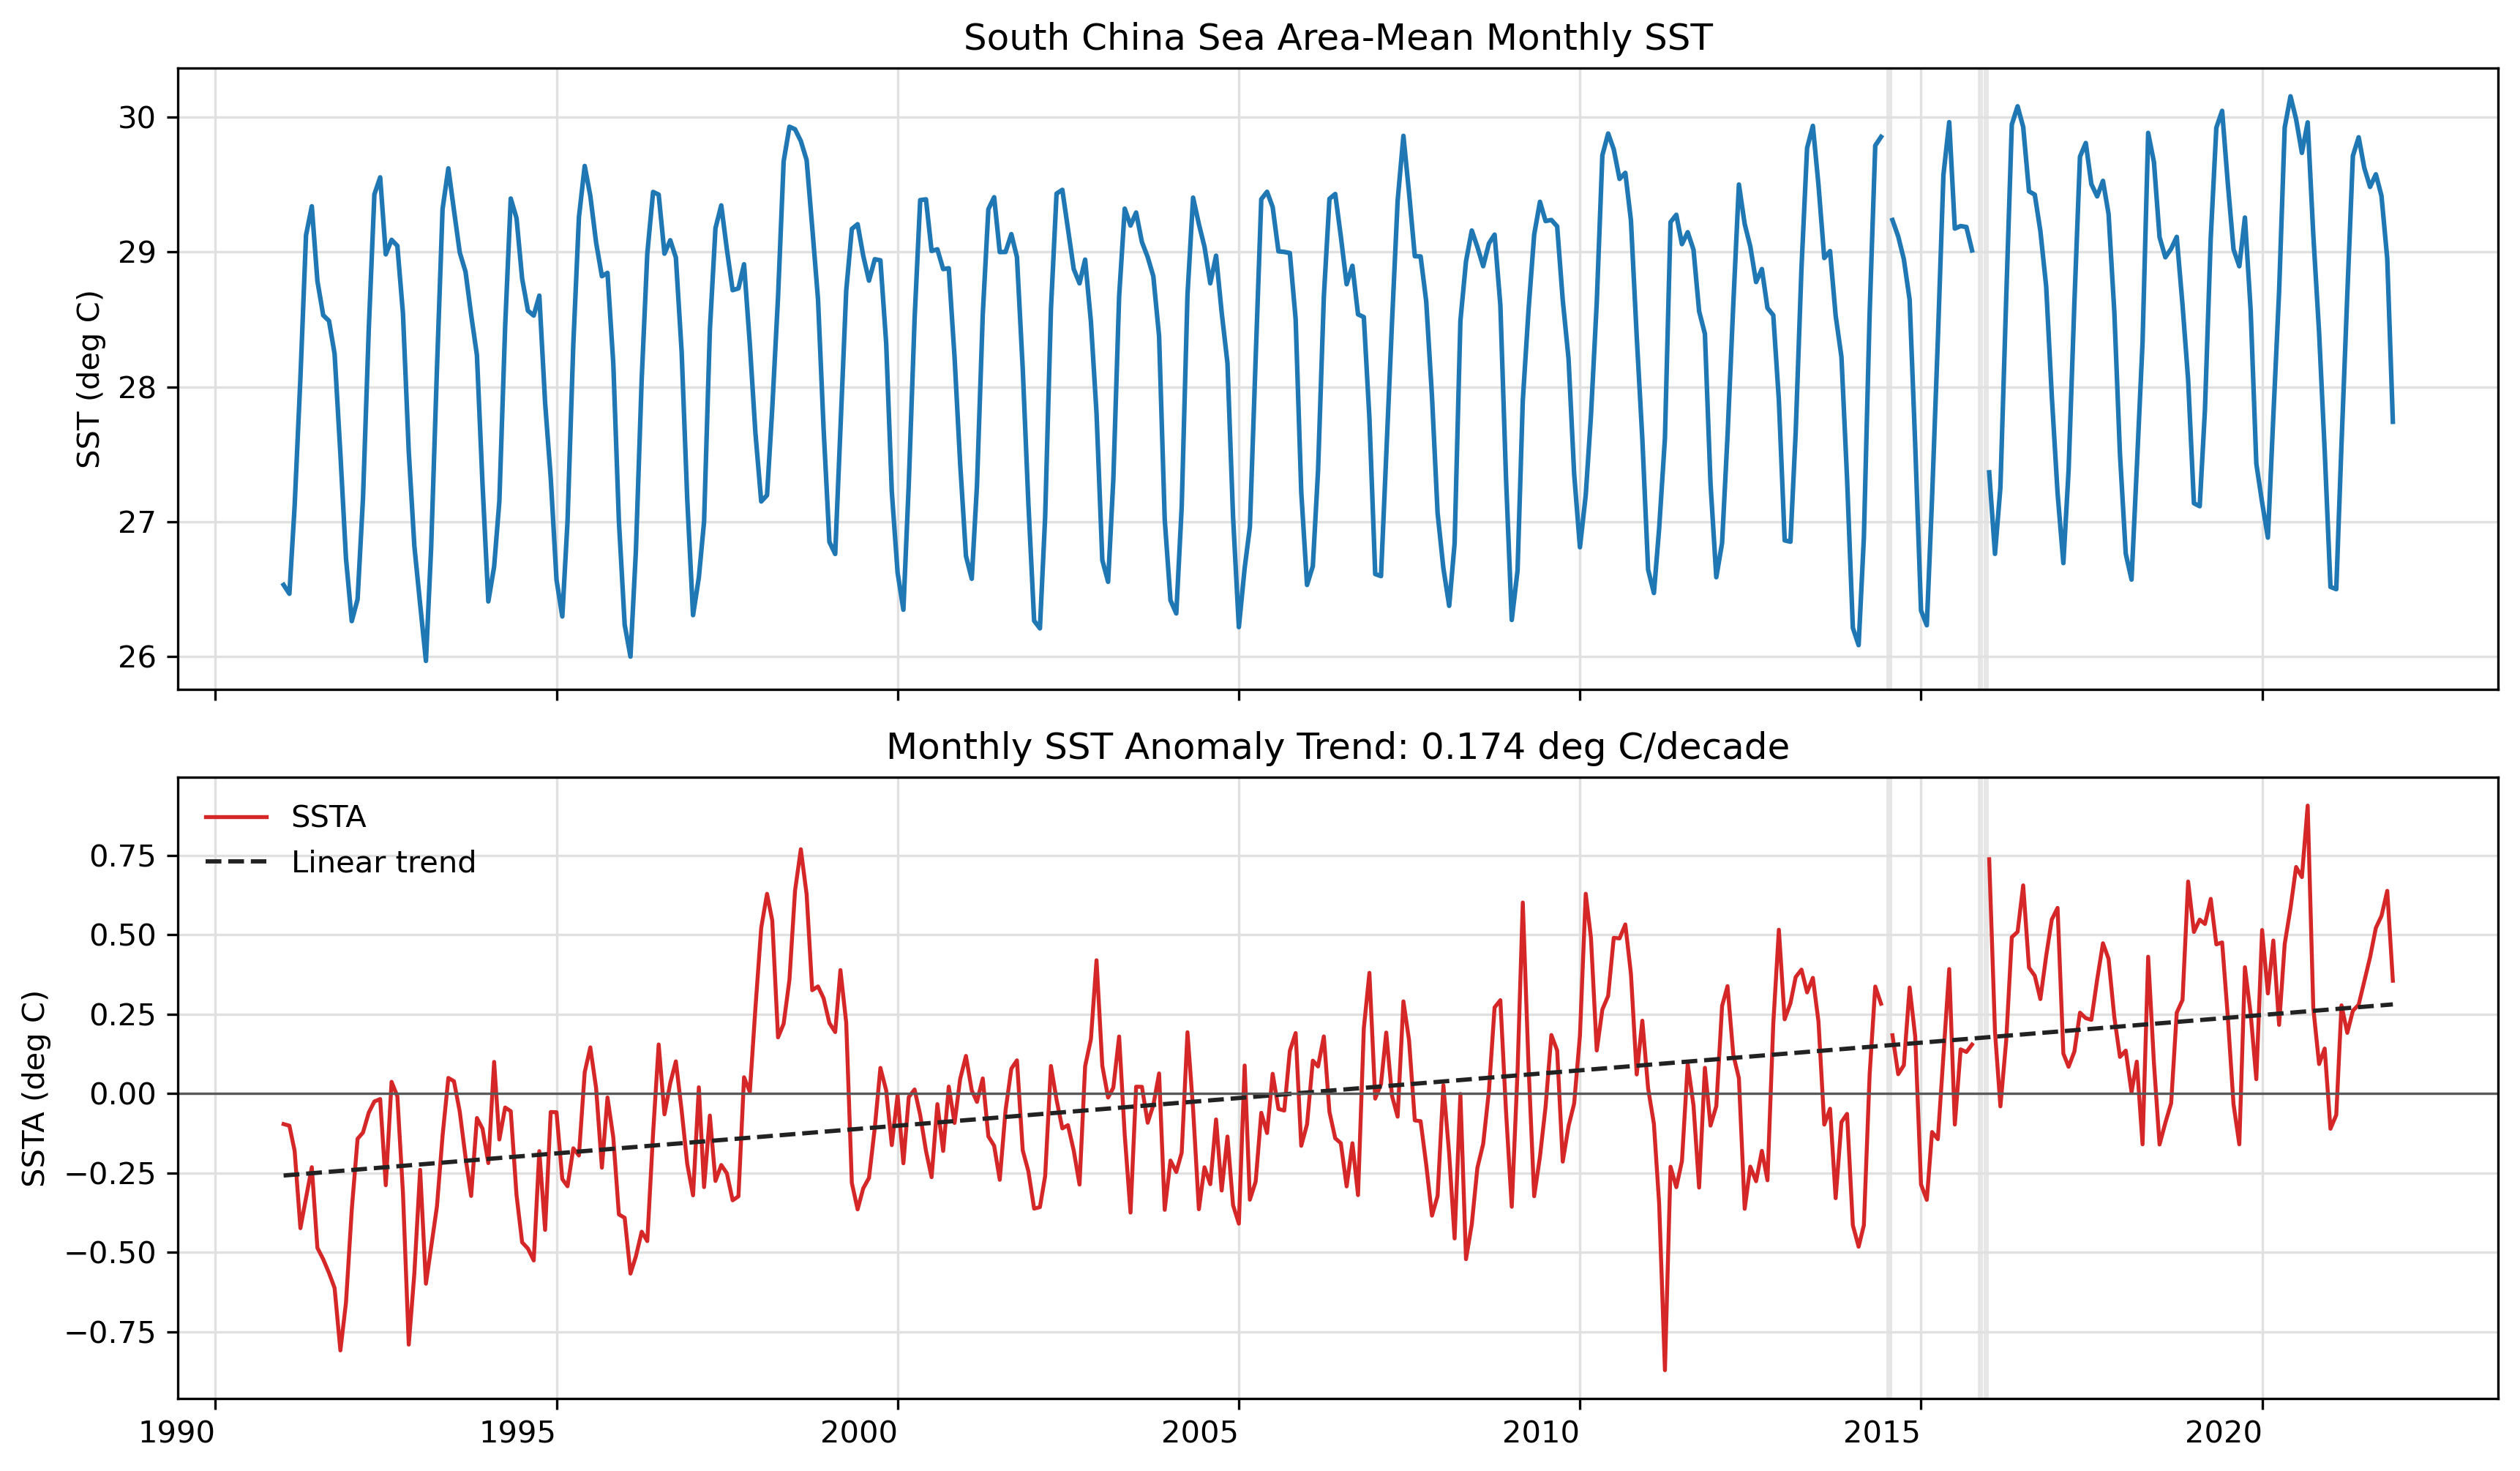
\includegraphics[width=\textwidth]{sst_area_mean_timeseries.png}
\caption{南海区域平均月尺度 SST 与 SSTA 时间序列}
\end{figure}

\begin{table}[H]
\centering
\caption{区域平均增暖和海洋热浪风险趋势摘要}
\resizebox{\textwidth}{!}{\begin{tabular}{lcccc}
\hline
指标 & 趋势/10年 & 线性变化量 & $p$ 值 & $n$ \\
\hline
区域平均 SST & 0.191 & 0.589 & 0.003 & 369 \\
区域平均 SSTA & 0.174 & 0.539 & 1.24e-25 & 369 \\
MHW 频次 & 1.308 & 3.923 & 3.40e-04 & 31 \\
MHW 总天数 & 13.381 & 40.144 & 0.002 & 31 \\
MHW 累计强度 & 15.176 & 45.528 & 0.003 & 31 \\
\hline
\end{tabular}
}
\end{table}

\subsection{季节循环与空间格局说明阈值建模必要性}
图 3 给出了区域平均 SST 月气候态。南海 SST 在春季快速升高，夏季维持高值，冬季受东北季风和海气热通量影响明显降低。这一季节循环说明，异常高温必须相对于逐月或逐日气候态定义，不能使用全年统一温度阈值。

\begin{figure}[H]
\centering
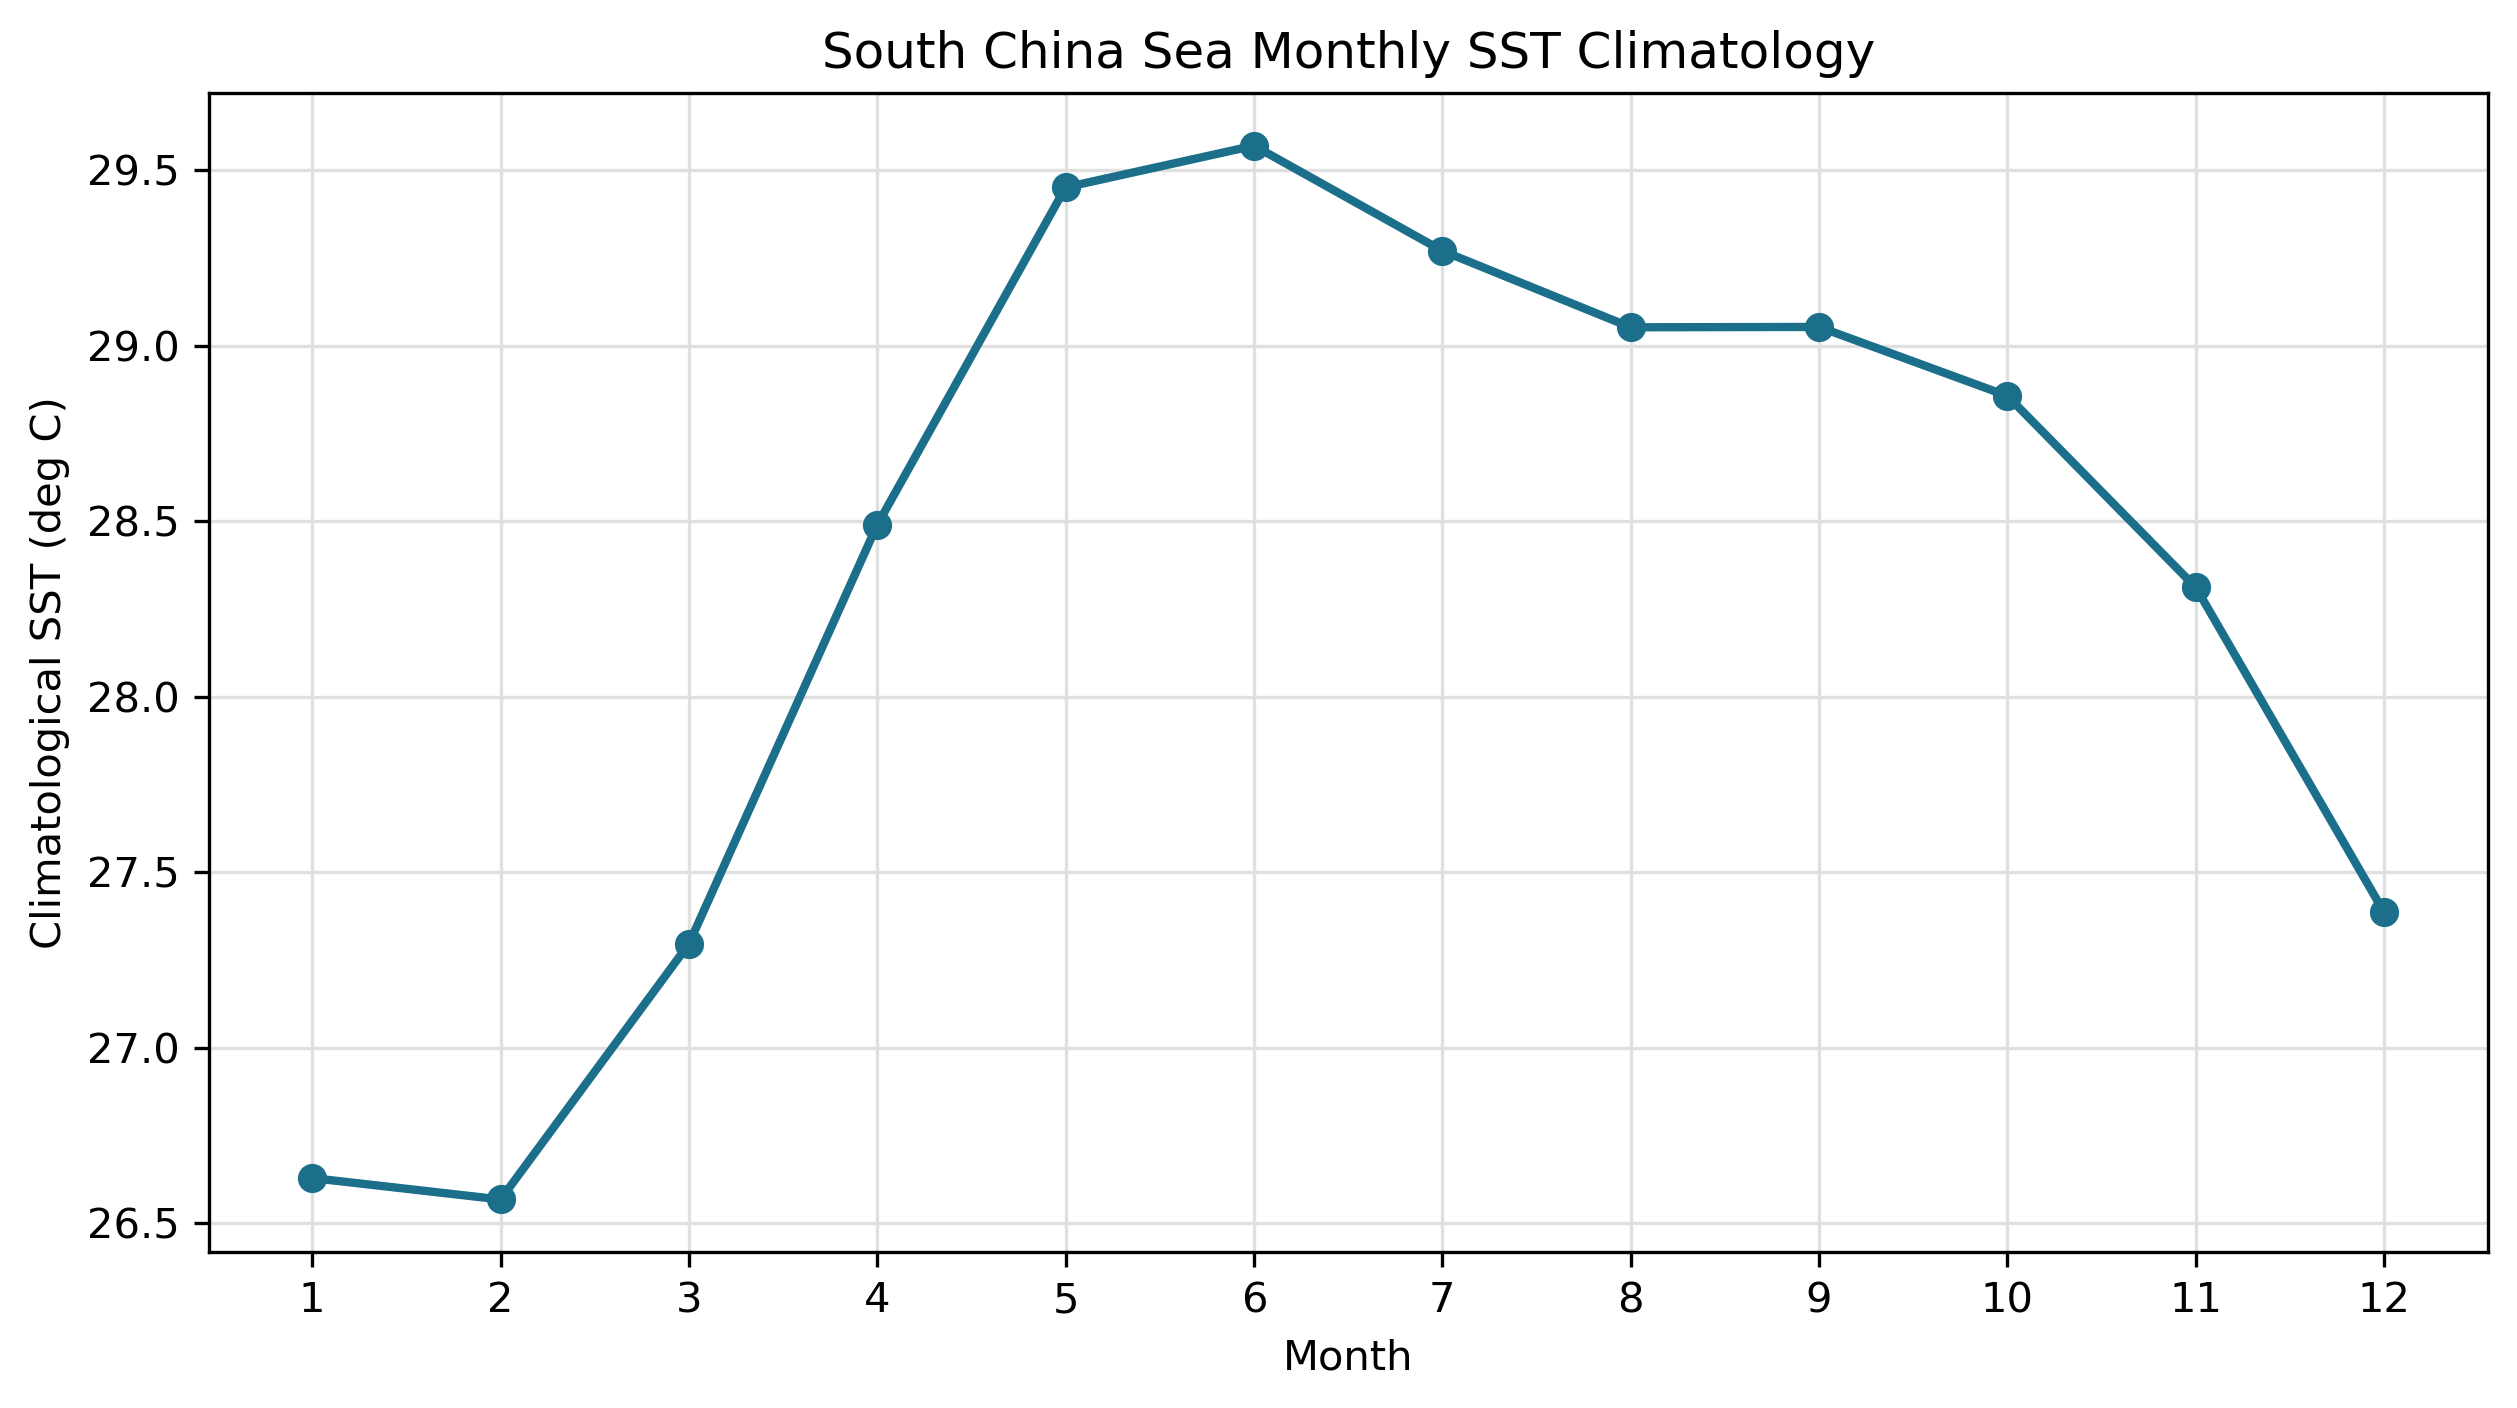
\includegraphics[width=0.78\textwidth]{sst_climatology_cycle.png}
\caption{南海区域平均月尺度 SST 气候态季节循环}
\end{figure}

图 4 显示多年平均 SST 和 SSTA 趋势空间分布。平均态上，低纬和南部海域 SST 较高，北部陆架相对较低；趋势场则表明增暖并非空间均匀过程，部分陆架、近岸和中南部海域的正趋势更突出。该空间差异提示，全区平均值只能刻画整体背景，若要服务风险管理，还需要进一步开展分区比较。

\begin{figure}[H]
\centering
\begin{subfigure}{0.48\textwidth}
\centering
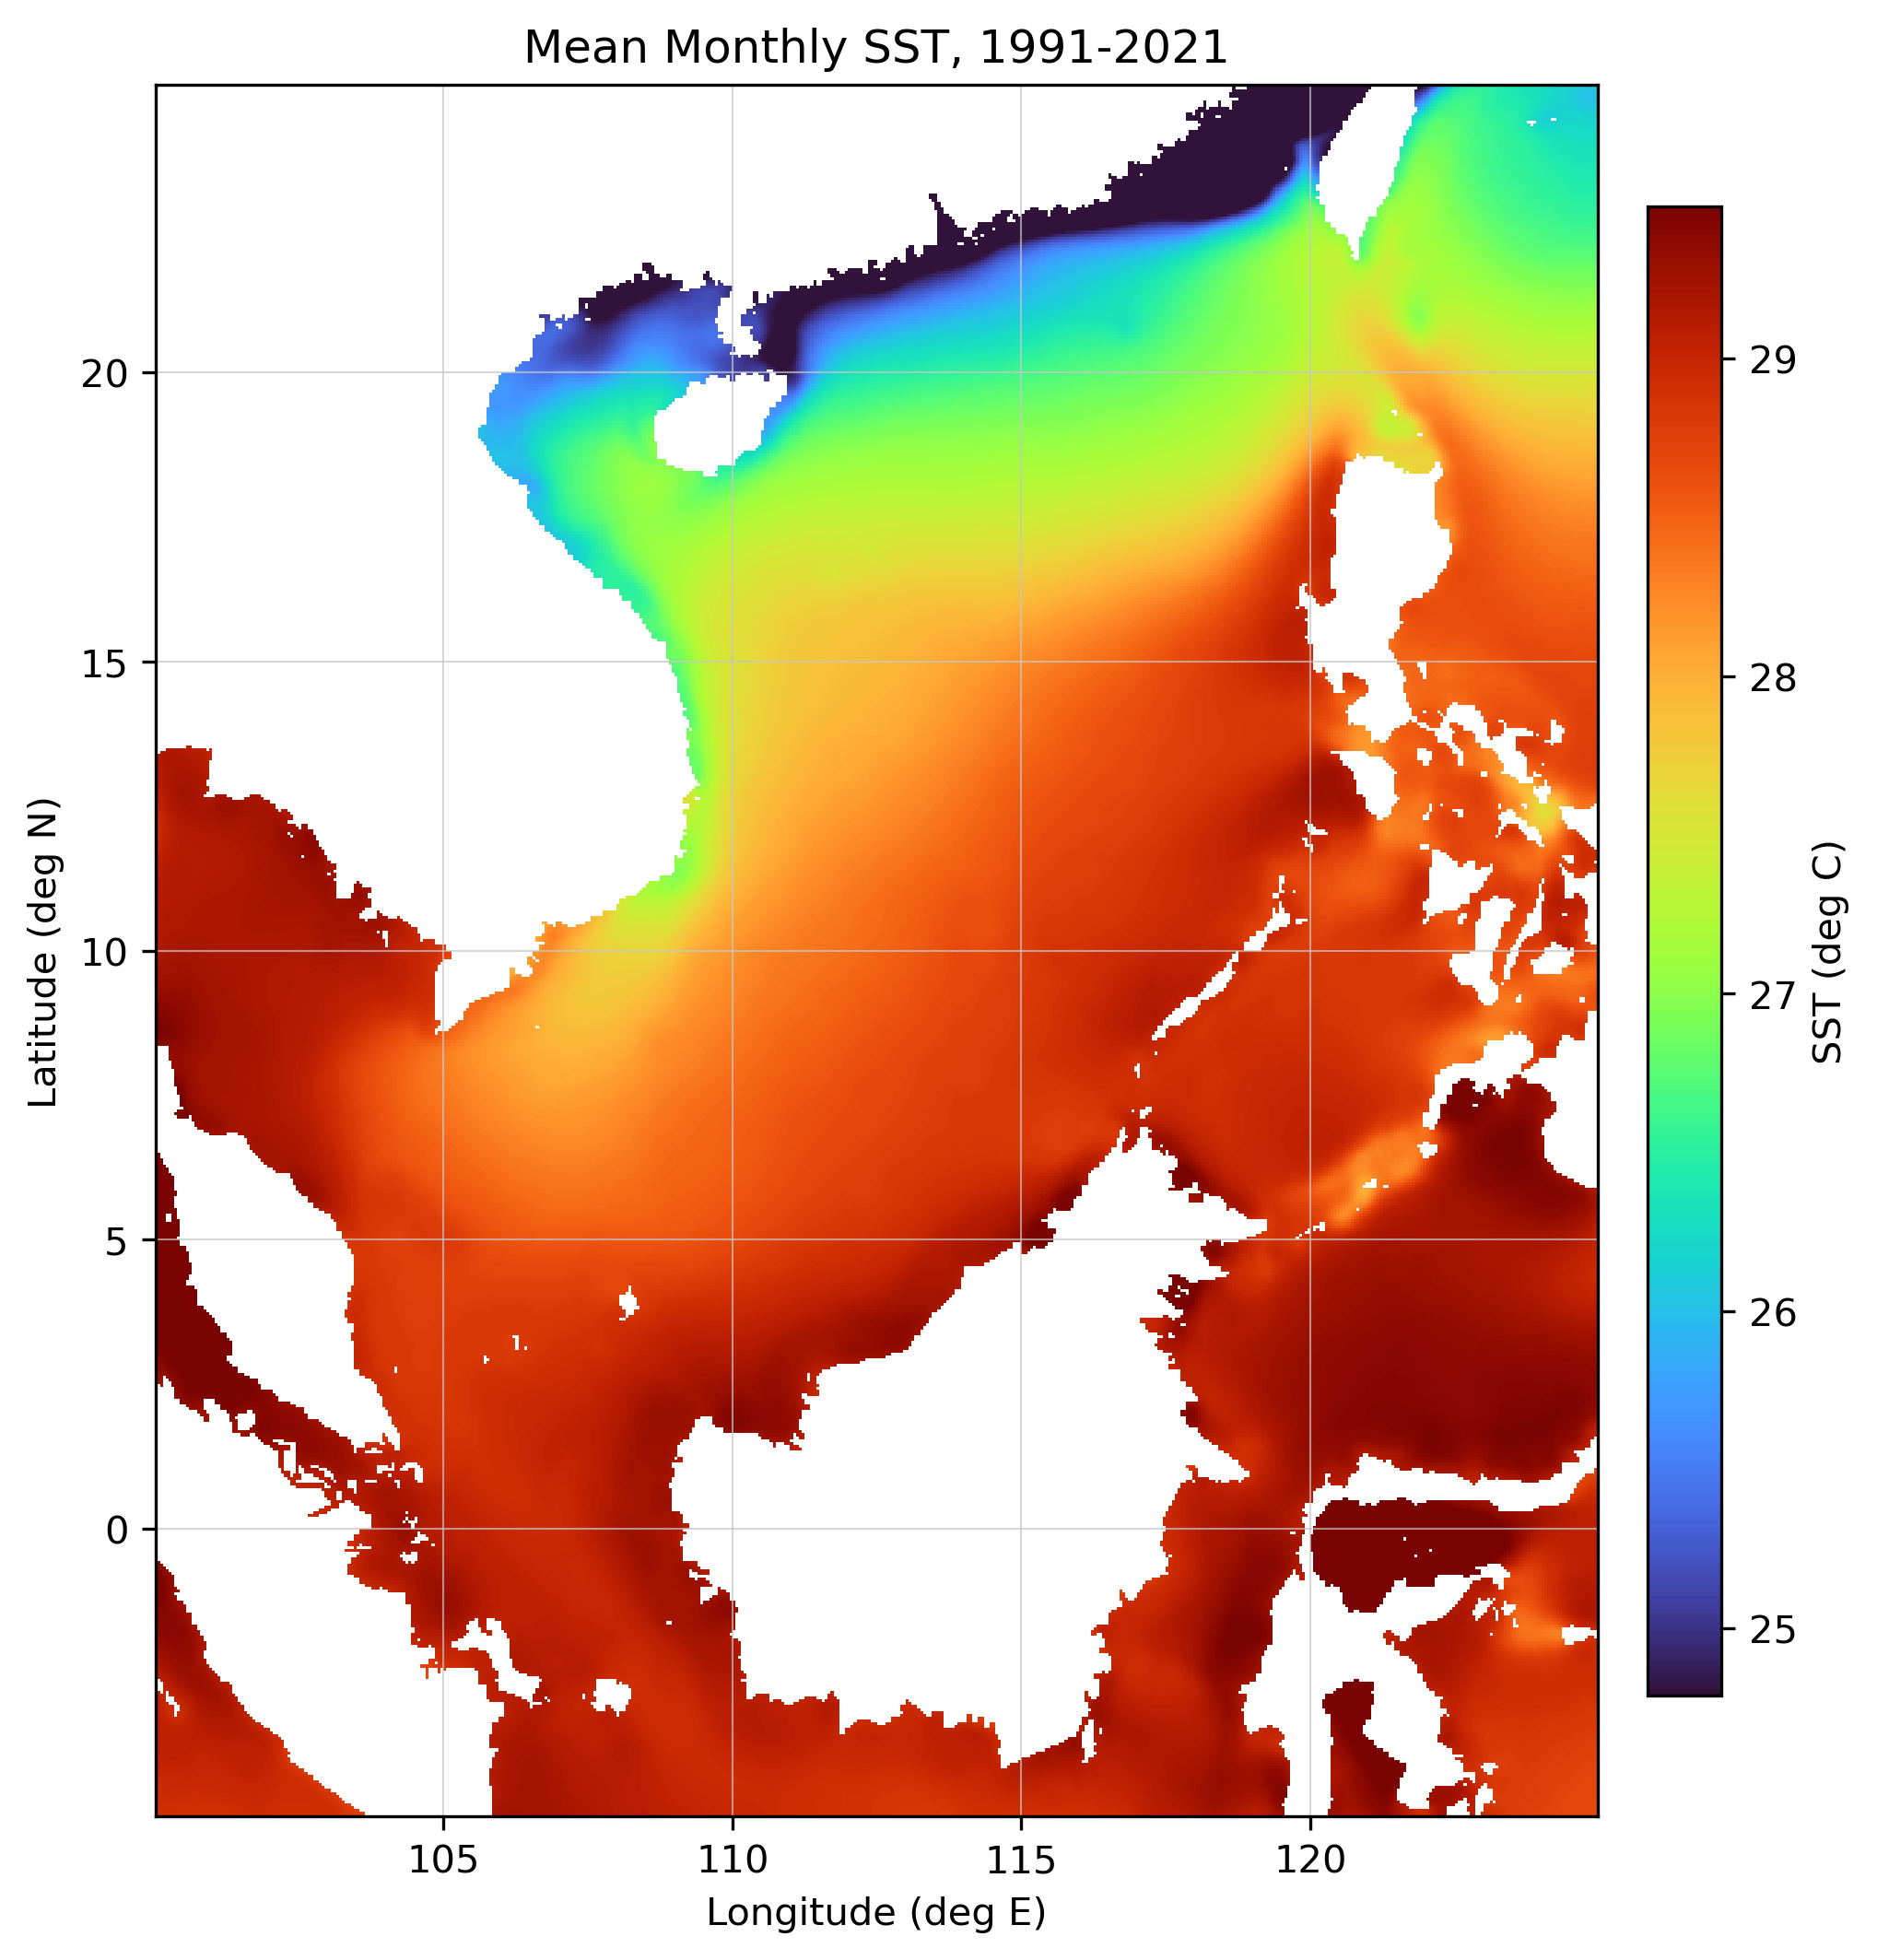
\includegraphics[width=\textwidth]{sst_mean_map.png}
\caption{多年平均 SST}
\end{subfigure}
\hfill
\begin{subfigure}{0.48\textwidth}
\centering
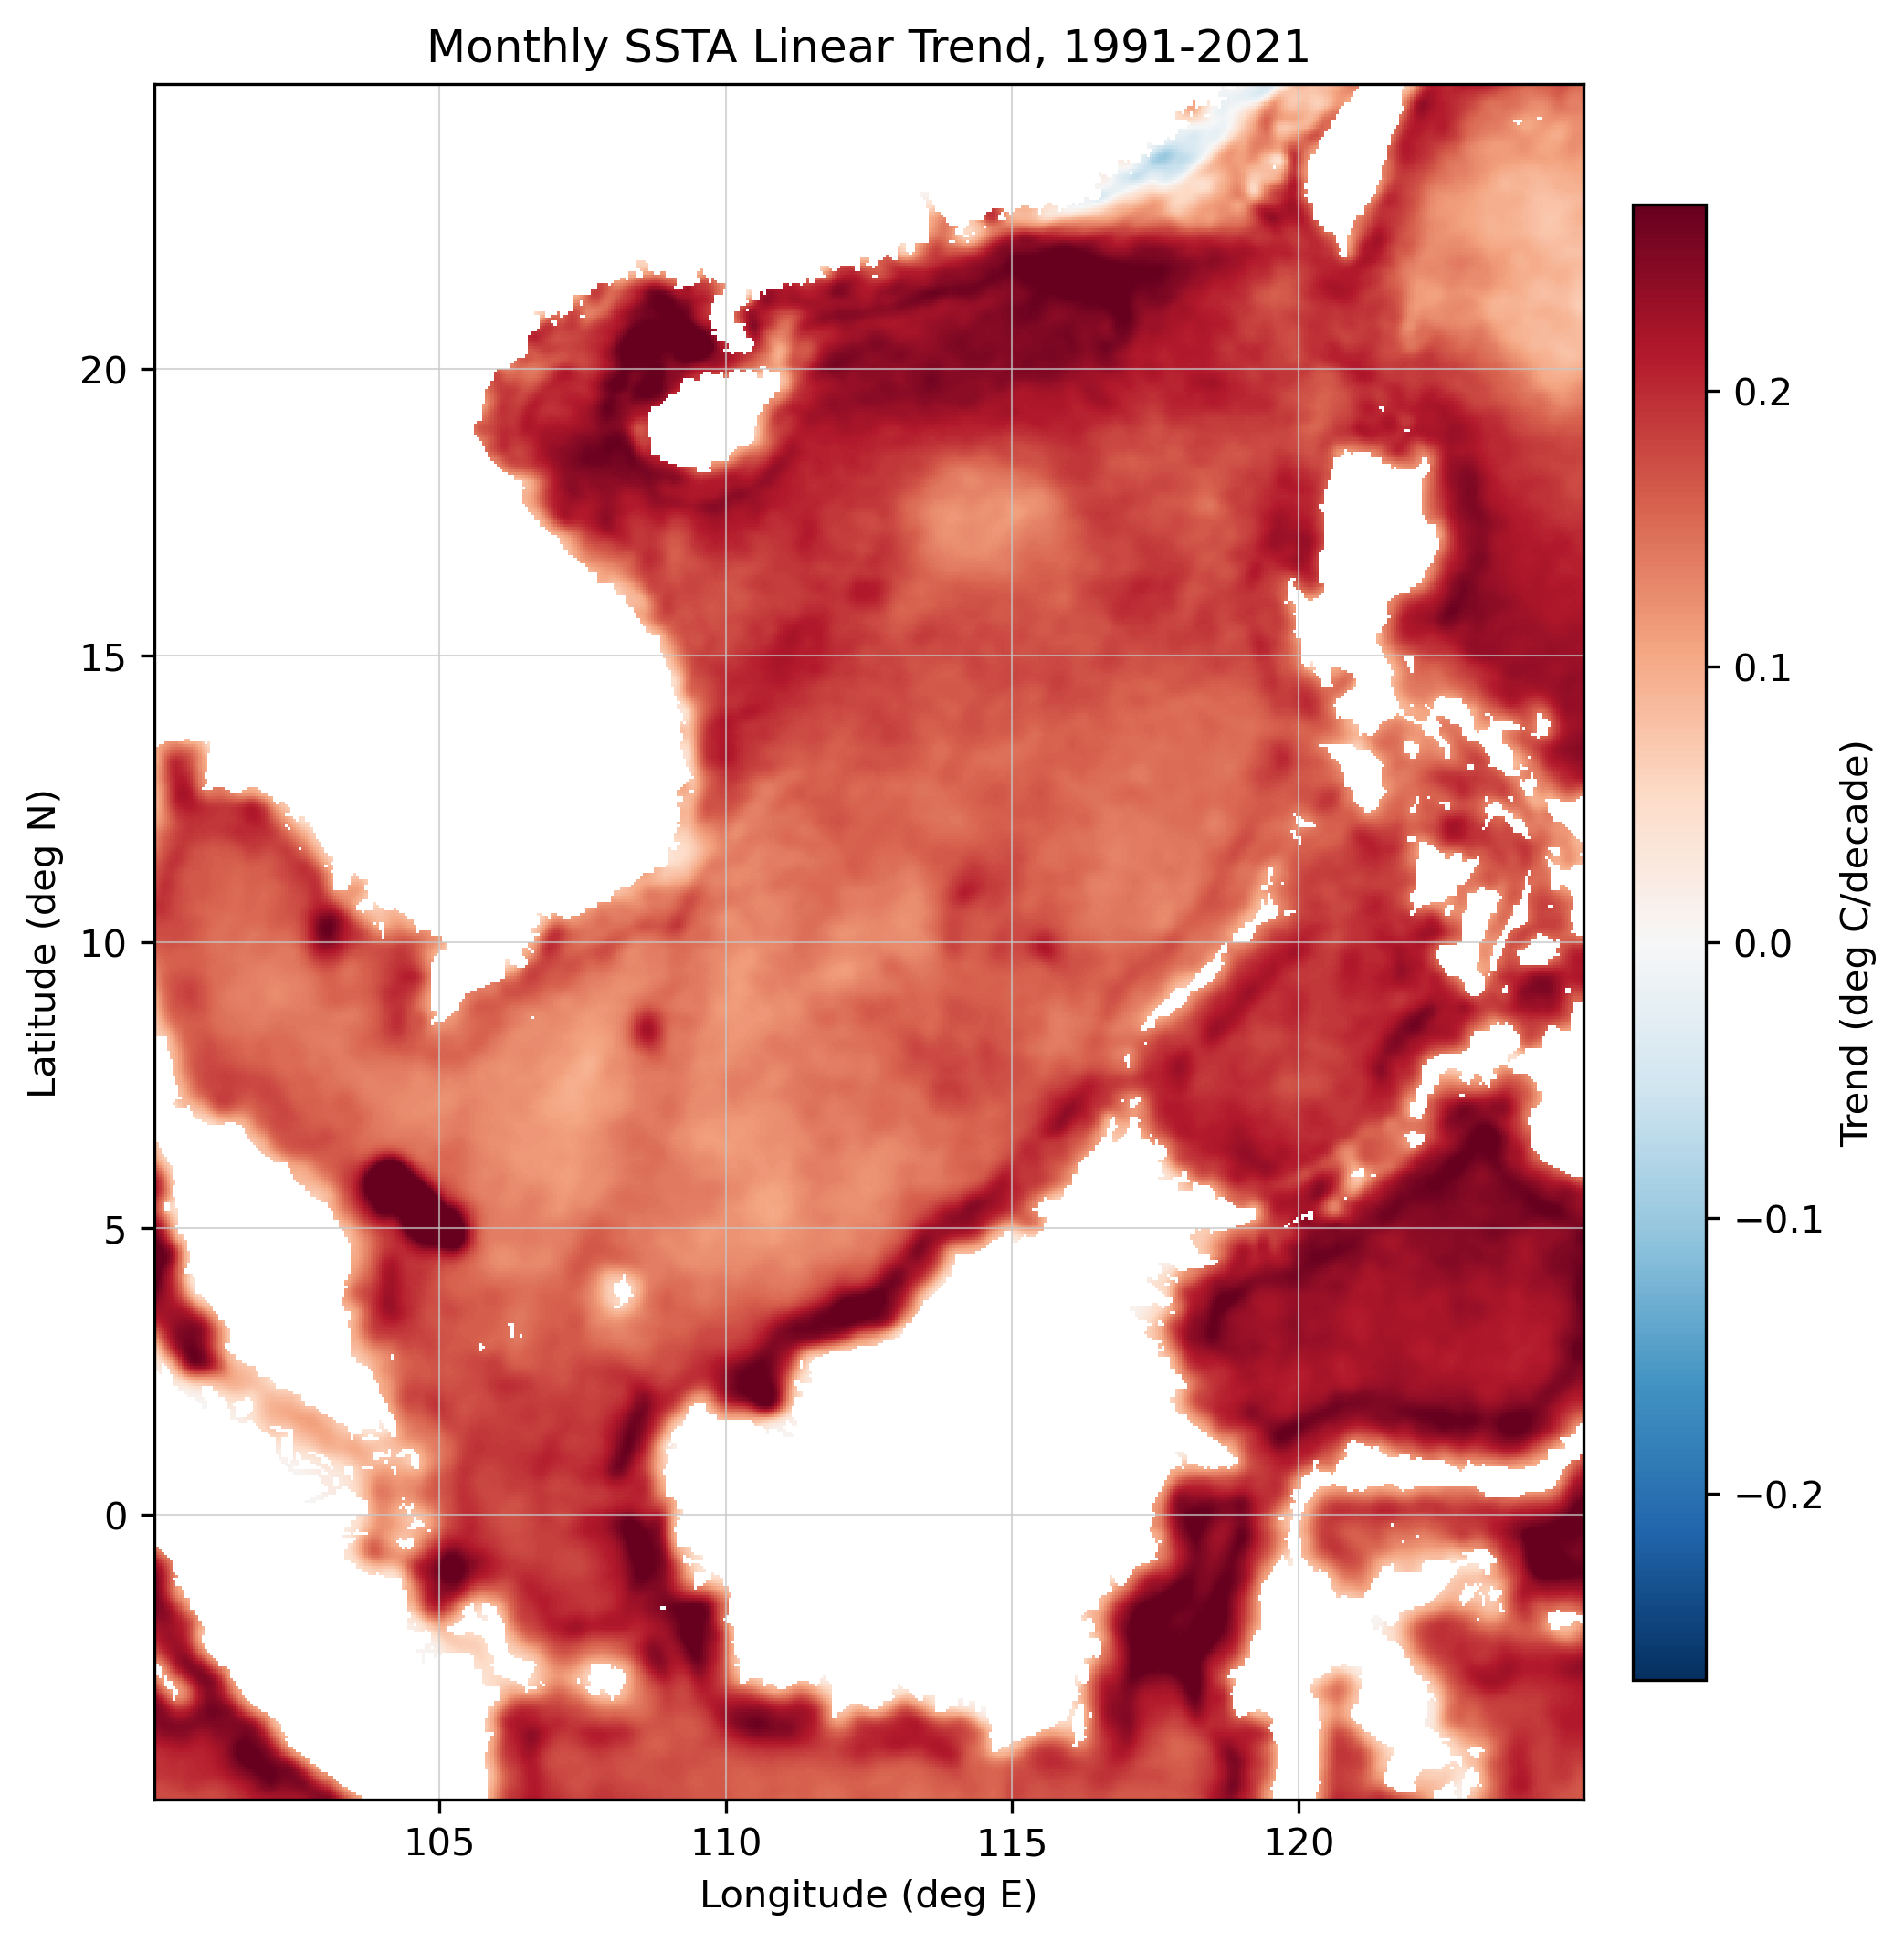
\includegraphics[width=\textwidth]{ssta_trend_map.png}
\caption{SSTA 线性趋势}
\end{subfigure}
\caption{南海 SST 平均态和月尺度 SSTA 趋势空间分布}
\end{figure}

\subsection{分区趋势揭示增暖空间异质性}
表 3 和图 5 给出了五个分区的 SSTA 与 MHW 指标趋势。SSTA 趋势在所有分区均为显著正值，其中北部陆架为 $0.187\,^{\circ}\mathrm{C}/10a$，东部外海为 $0.177\,^{\circ}\mathrm{C}/10a$，中部海盆、南部南海和西部近岸也均超过 $0.16\,^{\circ}\mathrm{C}/10a$。这说明南海增暖具有全域一致性，但不同海区的幅度并不相同。北部陆架同时表现出较高的 MHW 总天数趋势和累计强度趋势，说明该区不仅平均态增暖明显，极端高温暴露也更值得关注。

\begin{table}[H]
\centering
\caption{南海分区增暖与海洋热浪趋势摘要}
\resizebox{\textwidth}{!}{\begin{tabular}{lcccc}
\hline
分区 & SSTA趋势 & MHW总天数趋势 & MHW累计强度趋势 & 显著性判断 \\
 & ($^\circ$C/10年) & (天/10年) & ($^\circ$C$\cdot$天/10年) &  \\
\hline
北部陆架 & 0.187 & 14.547 & 21.182 & SSTA ***; 天数 ***; 强度 ** \\
中部海盆 & 0.162 & 11.489 & 14.103 & SSTA ***; 天数 *; 强度 * \\
南部南海 & 0.166 & 13.265 & 13.622 & SSTA ***; 天数 *; 强度 * \\
西部近岸 & 0.161 & 13.853 & 17.080 & SSTA ***; 天数 **; 强度 ** \\
东部外海 & 0.177 & 12.651 & 14.991 & SSTA ***; 天数 **; 强度 ** \\
\hline
\end{tabular}
}
\end{table}

\begin{figure}[H]
\centering
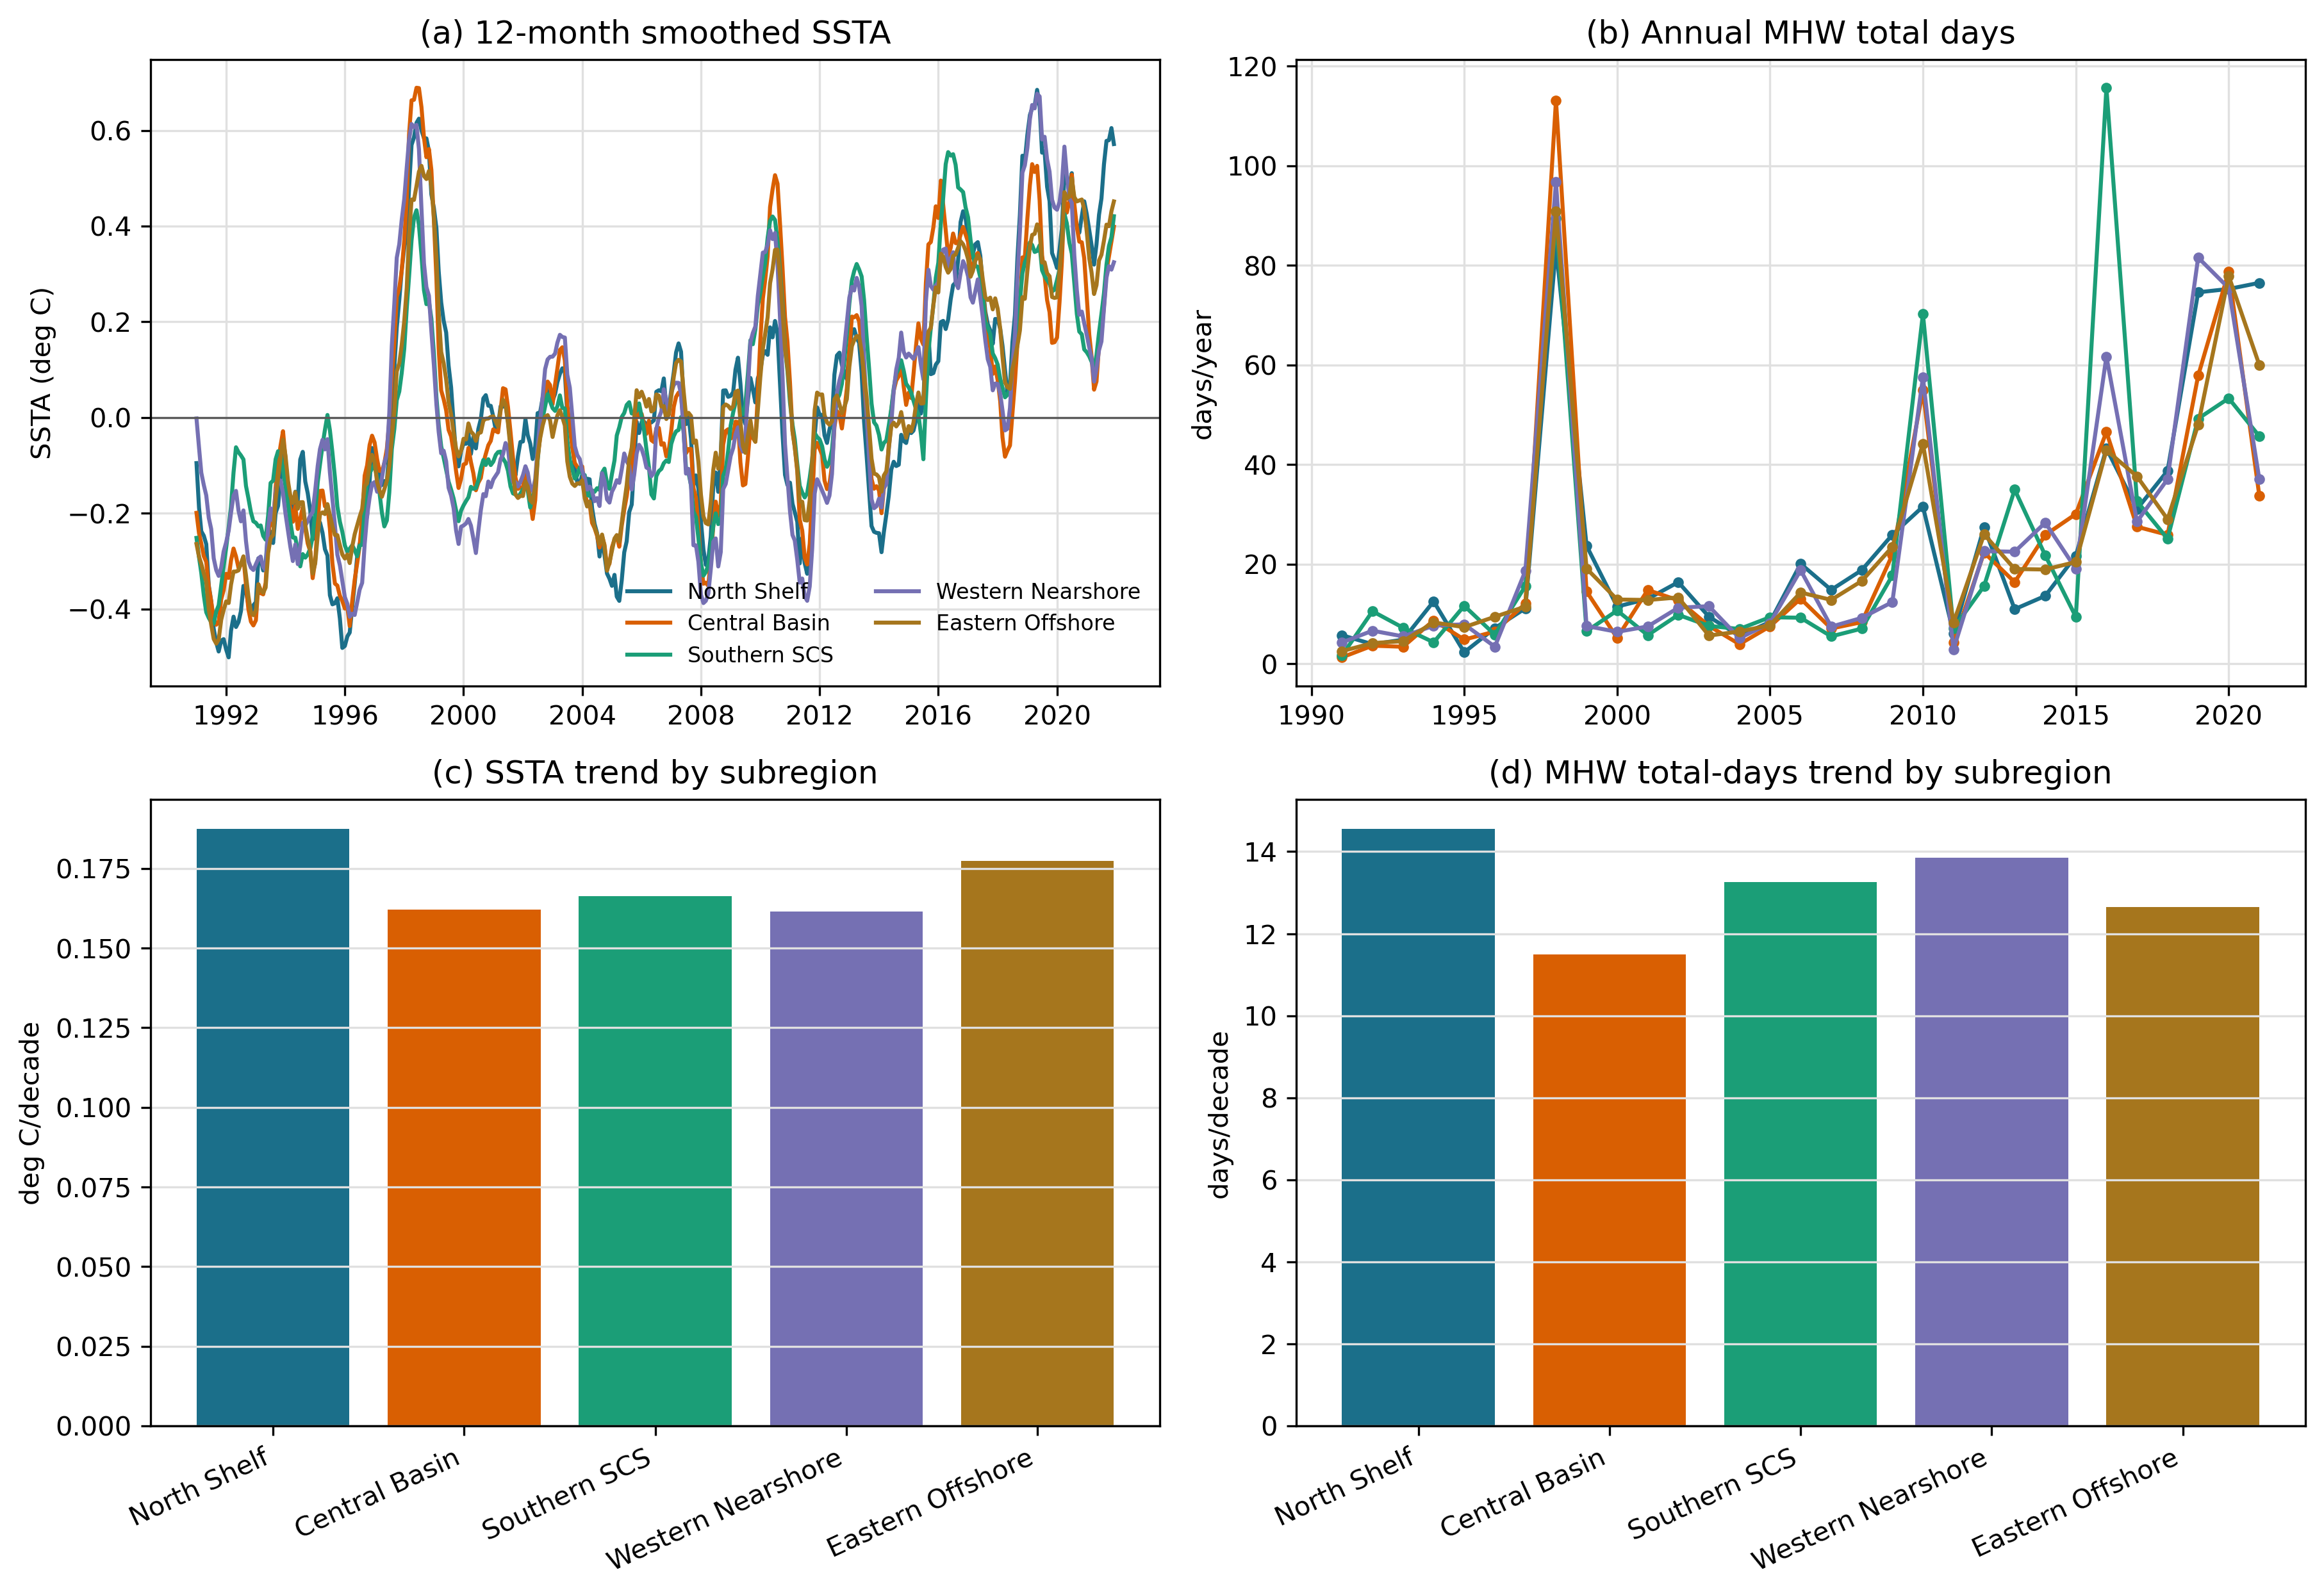
\includegraphics[width=\textwidth]{subregion_trend_panel.png}
\caption{南海分区 SSTA 与 MHW 总天数变化}
\end{figure}

\subsection{稳健性检验确认趋势方向一致}
表 4 和图 6 对主要指标进行 OLS、Theil-Sen 和 Kendall 检验比较。区域平均 SSTA 的 OLS 趋势为 $0.174\,^{\circ}\mathrm{C}/10a$，Theil-Sen 趋势为 $0.179\,^{\circ}\mathrm{C}/10a$，Kendall $\tau=0.351$ 且 $p<0.001$。MHW 频次、总天数、累计强度和最大强度也均表现为显著增加。OLS 和 Theil-Sen 趋势虽在数值上有差异，但方向一致，说明少数异常年份并未改变长期增强结论。

\begin{table}[H]
\centering
\caption{主要指标趋势稳健性检验}
\resizebox{\textwidth}{!}{\begin{tabular}{lcccccc}
\hline
指标 & 单位 & OLS趋势 & Theil-Sen趋势 & Kendall $\tau$ & $p$ 值 & 结论 \\
\hline
区域平均SSTA & $^\circ$C/10年 & 0.174 & 0.179 & 0.351 & $p<0.001$ & 显著增加 \\
MHW频次 & 次/10年 & 1.308 & 1.010 & 0.600 & $p<0.001$ & 显著增加 \\
MHW总天数 & 天/10年 & 13.381 & 9.544 & 0.617 & $p<0.001$ & 显著增加 \\
MHW累计强度 & $^\circ$C$\cdot$天/10年 & 15.176 & 11.582 & 0.600 & $p<0.001$ & 显著增加 \\
MHW最大强度 & $^\circ$C/10年 & 0.065 & 0.078 & 0.303 & $p<0.05$ & 显著增加 \\
\hline
\end{tabular}
}
\end{table}

\begin{figure}[H]
\centering
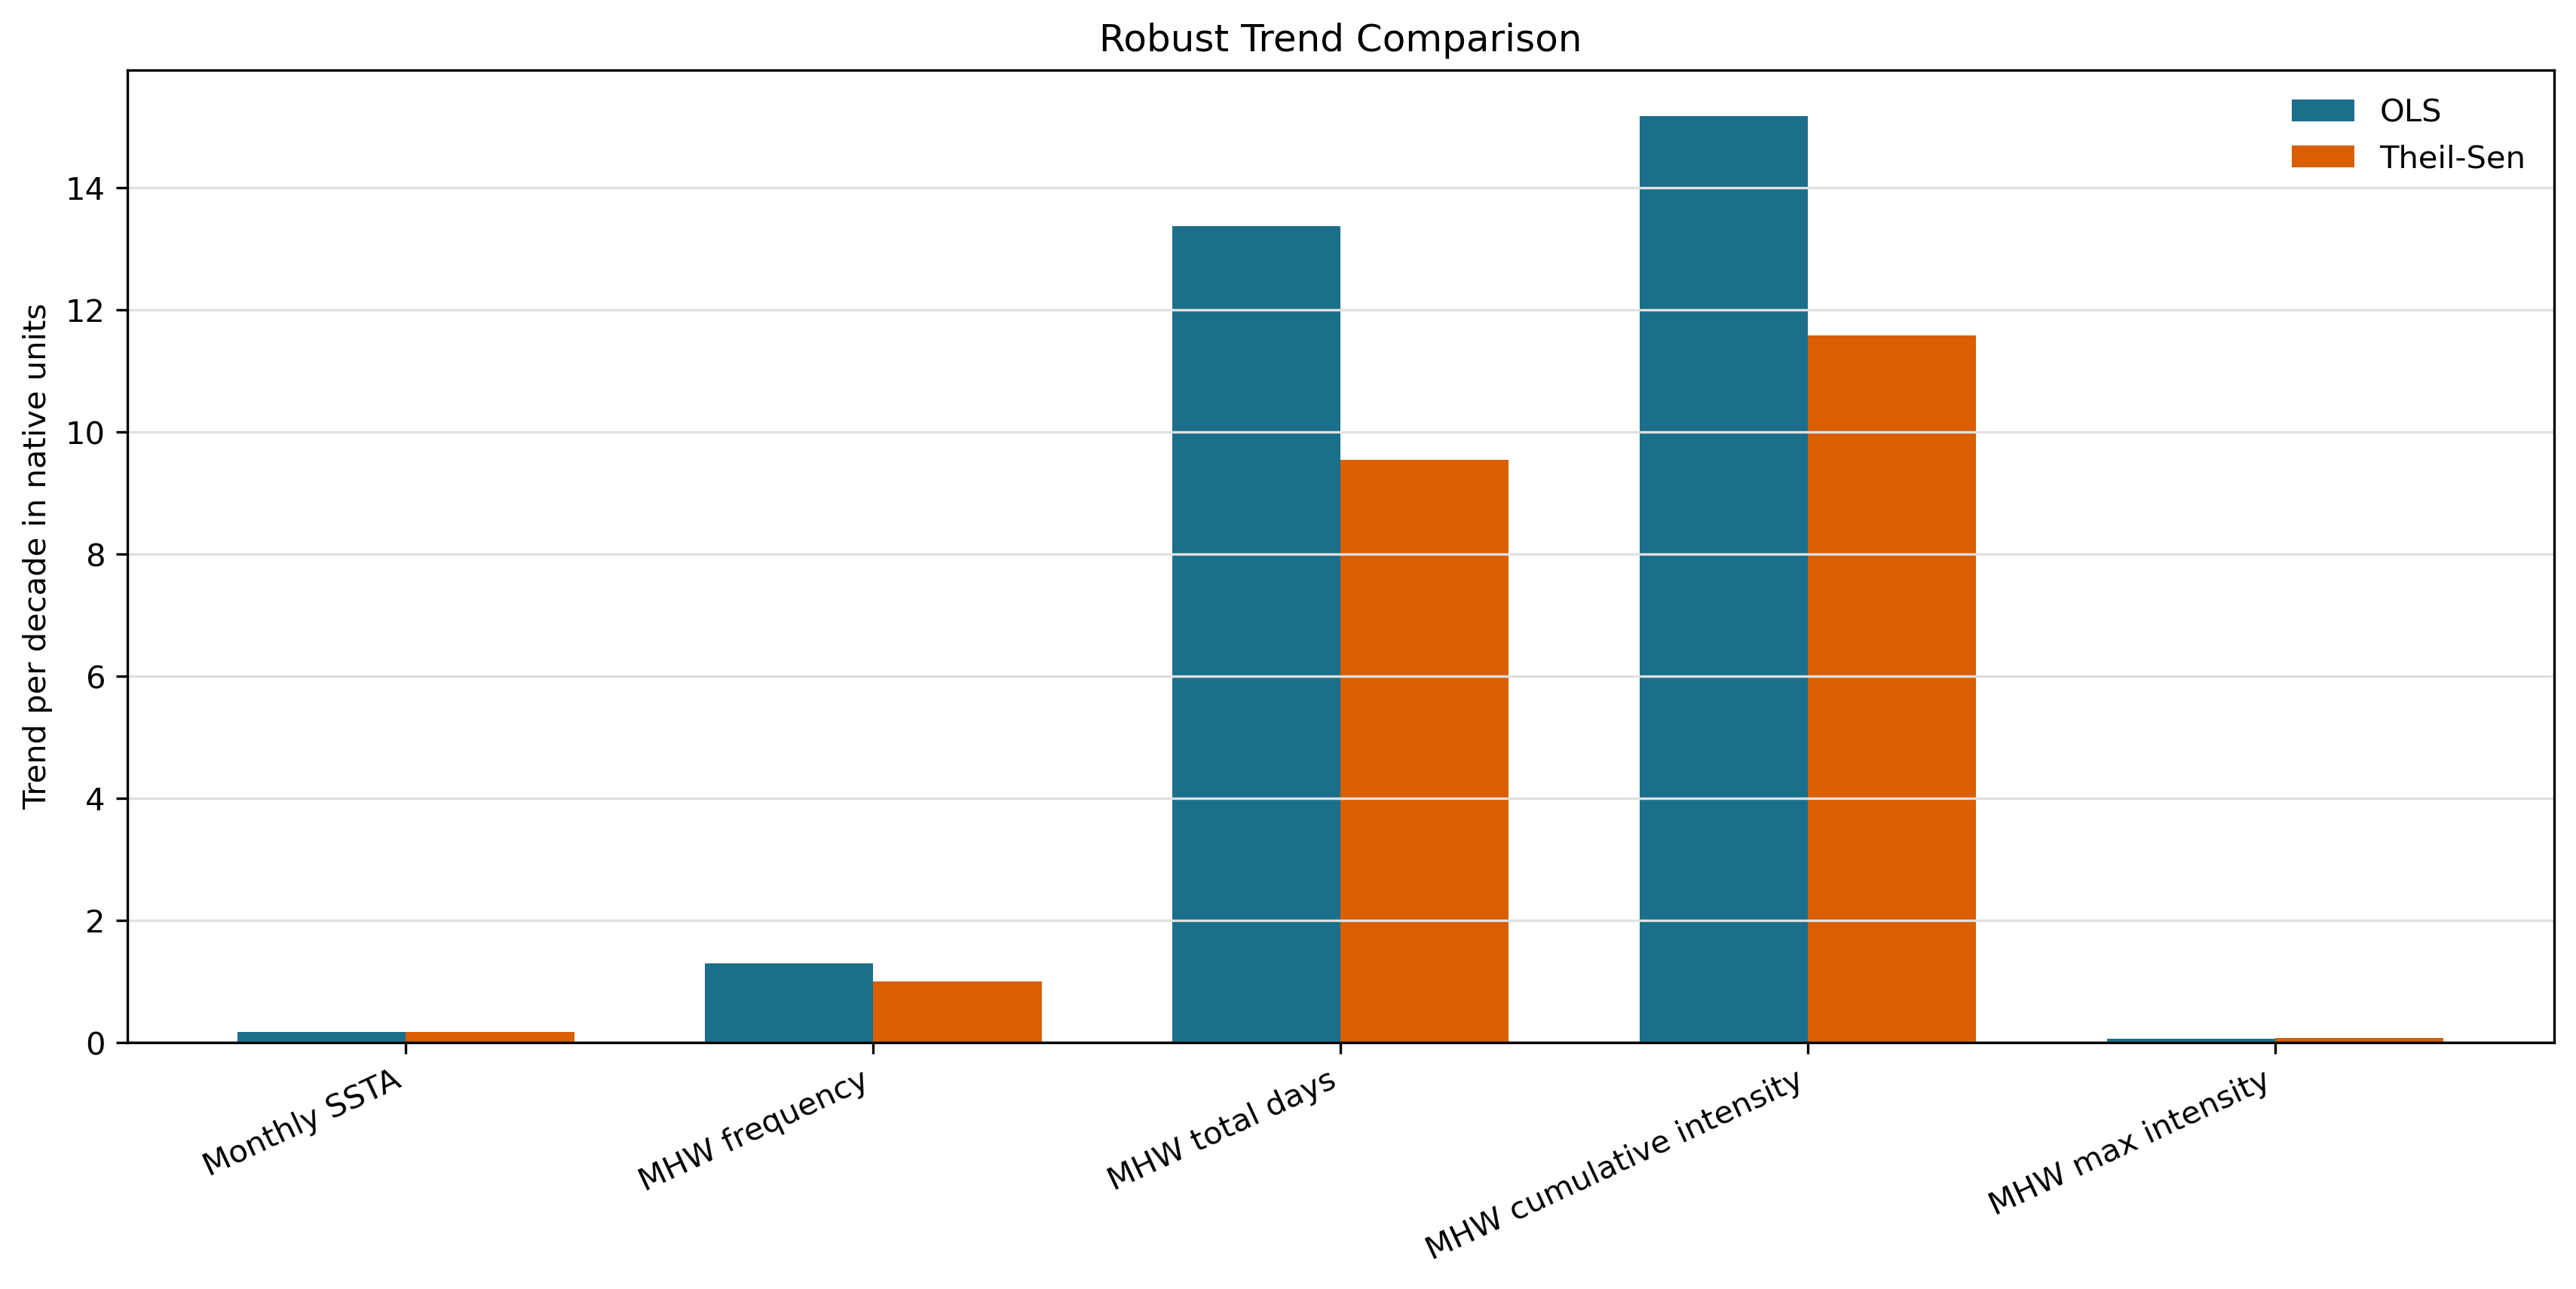
\includegraphics[width=0.86\textwidth]{robust_trend_comparison.png}
\caption{主要指标 OLS 与 Theil-Sen 趋势比较}
\end{figure}

本节结果表明，南海海表温度存在显著且稳健的长期增暖，并且不同海区增暖幅度不同。这为进一步分析持续性极端热事件奠定了平均态背景。

\section{南海海洋热浪风险演化}

\subsection{年度事件指标显示热风险增强}
图 7 展示区域平均年度 MHW 指标。与平均温度趋势相比，MHW 指标更直接反映异常高温暴露。1991--2021 年，区域平均 MHW 频次增加 $1.308$ 次/10年，总天数增加 $13.381$ 天/10年，累计强度增加 $15.176\,^{\circ}\mathrm{C}\cdot\mathrm{d}/10a$。这表明南海增暖已经转化为更高频、更持久的海洋高温事件，而不仅是平均态抬升。

\begin{figure}[H]
\centering
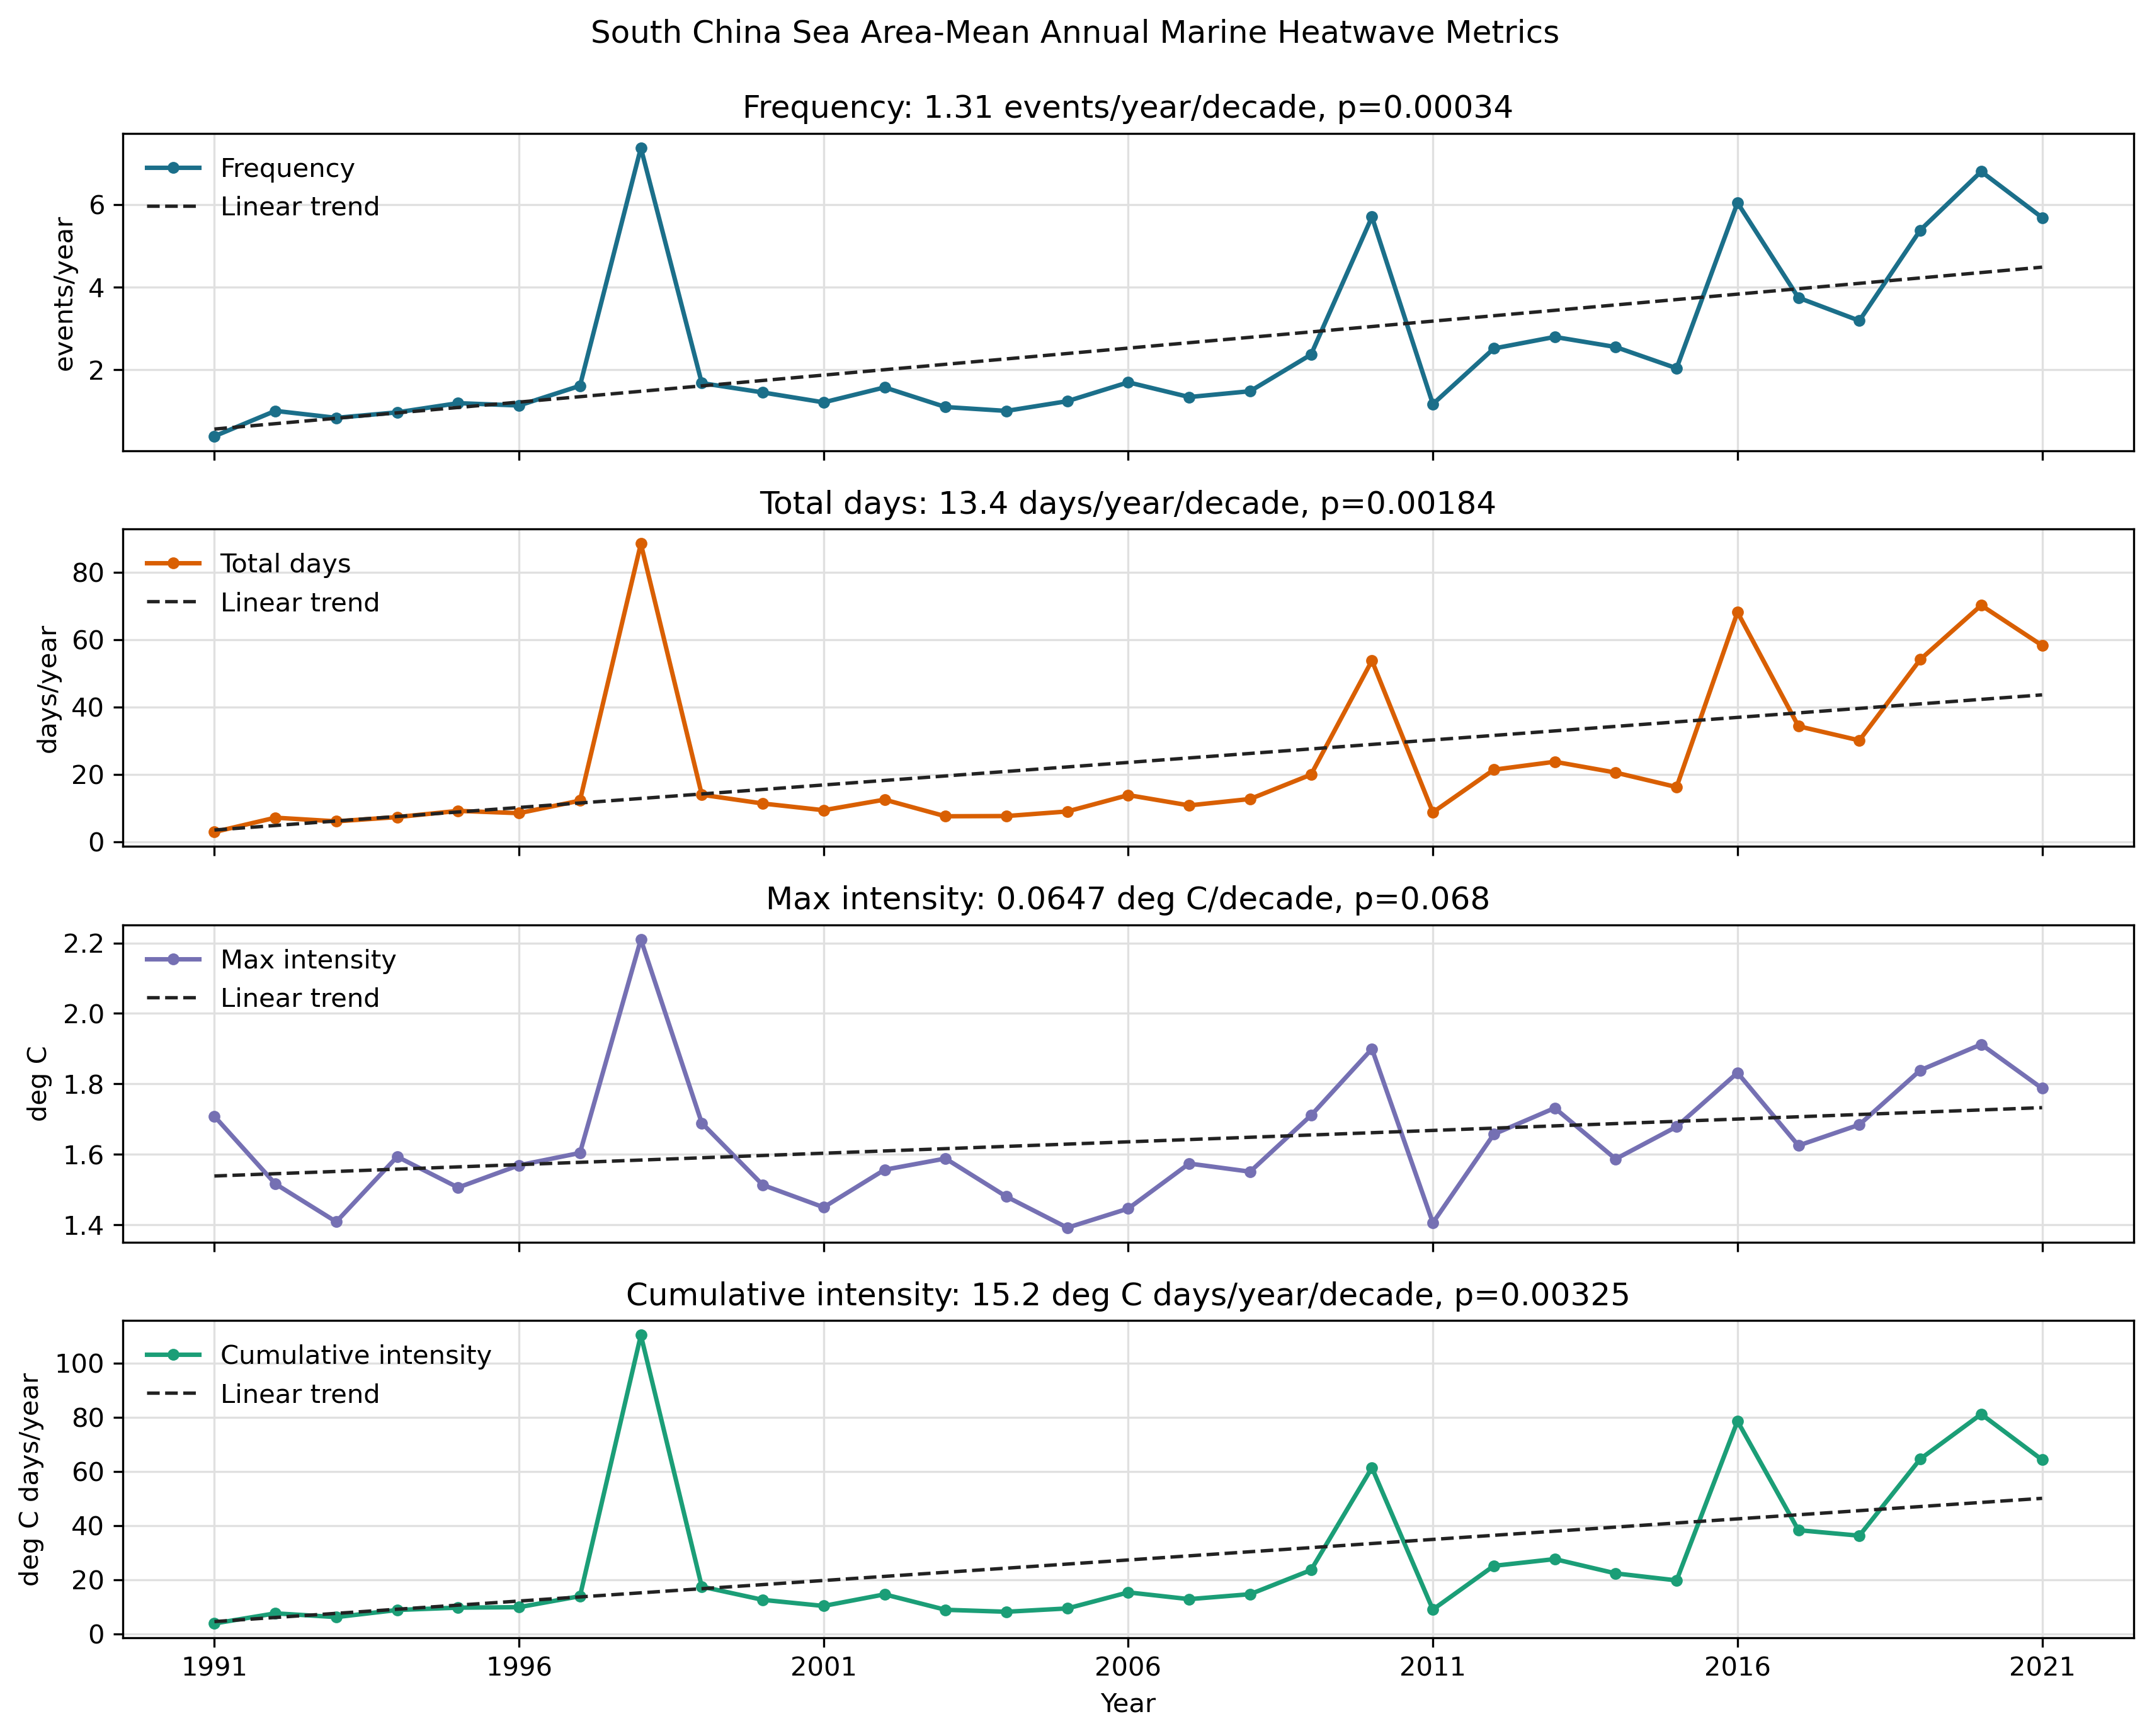
\includegraphics[width=\textwidth]{mhw_area_mean_timeseries.png}
\caption{南海区域平均年度海洋热浪指标时间序列}
\end{figure}

\subsection{总天数和累计强度刻画持续性热胁迫}
MHW 频次反映事件发生次数，总天数反映暴露时长，累计强度则综合持续时间和强度，是更接近生态热胁迫的指标。图 8 显示多年平均 MHW 总天数和总天数趋势，图 9 显示累计强度趋势。多年平均总天数较高区域与多年平均 SST 最高区域并不完全重合，说明热浪风险受当地气候态阈值、持续性和年际变率共同影响。趋势场中大部分海洋格点表现为正趋势，说明热浪增强不是少数离散格点造成的局地现象。

\begin{figure}[H]
\centering
\begin{subfigure}{0.48\textwidth}
\centering
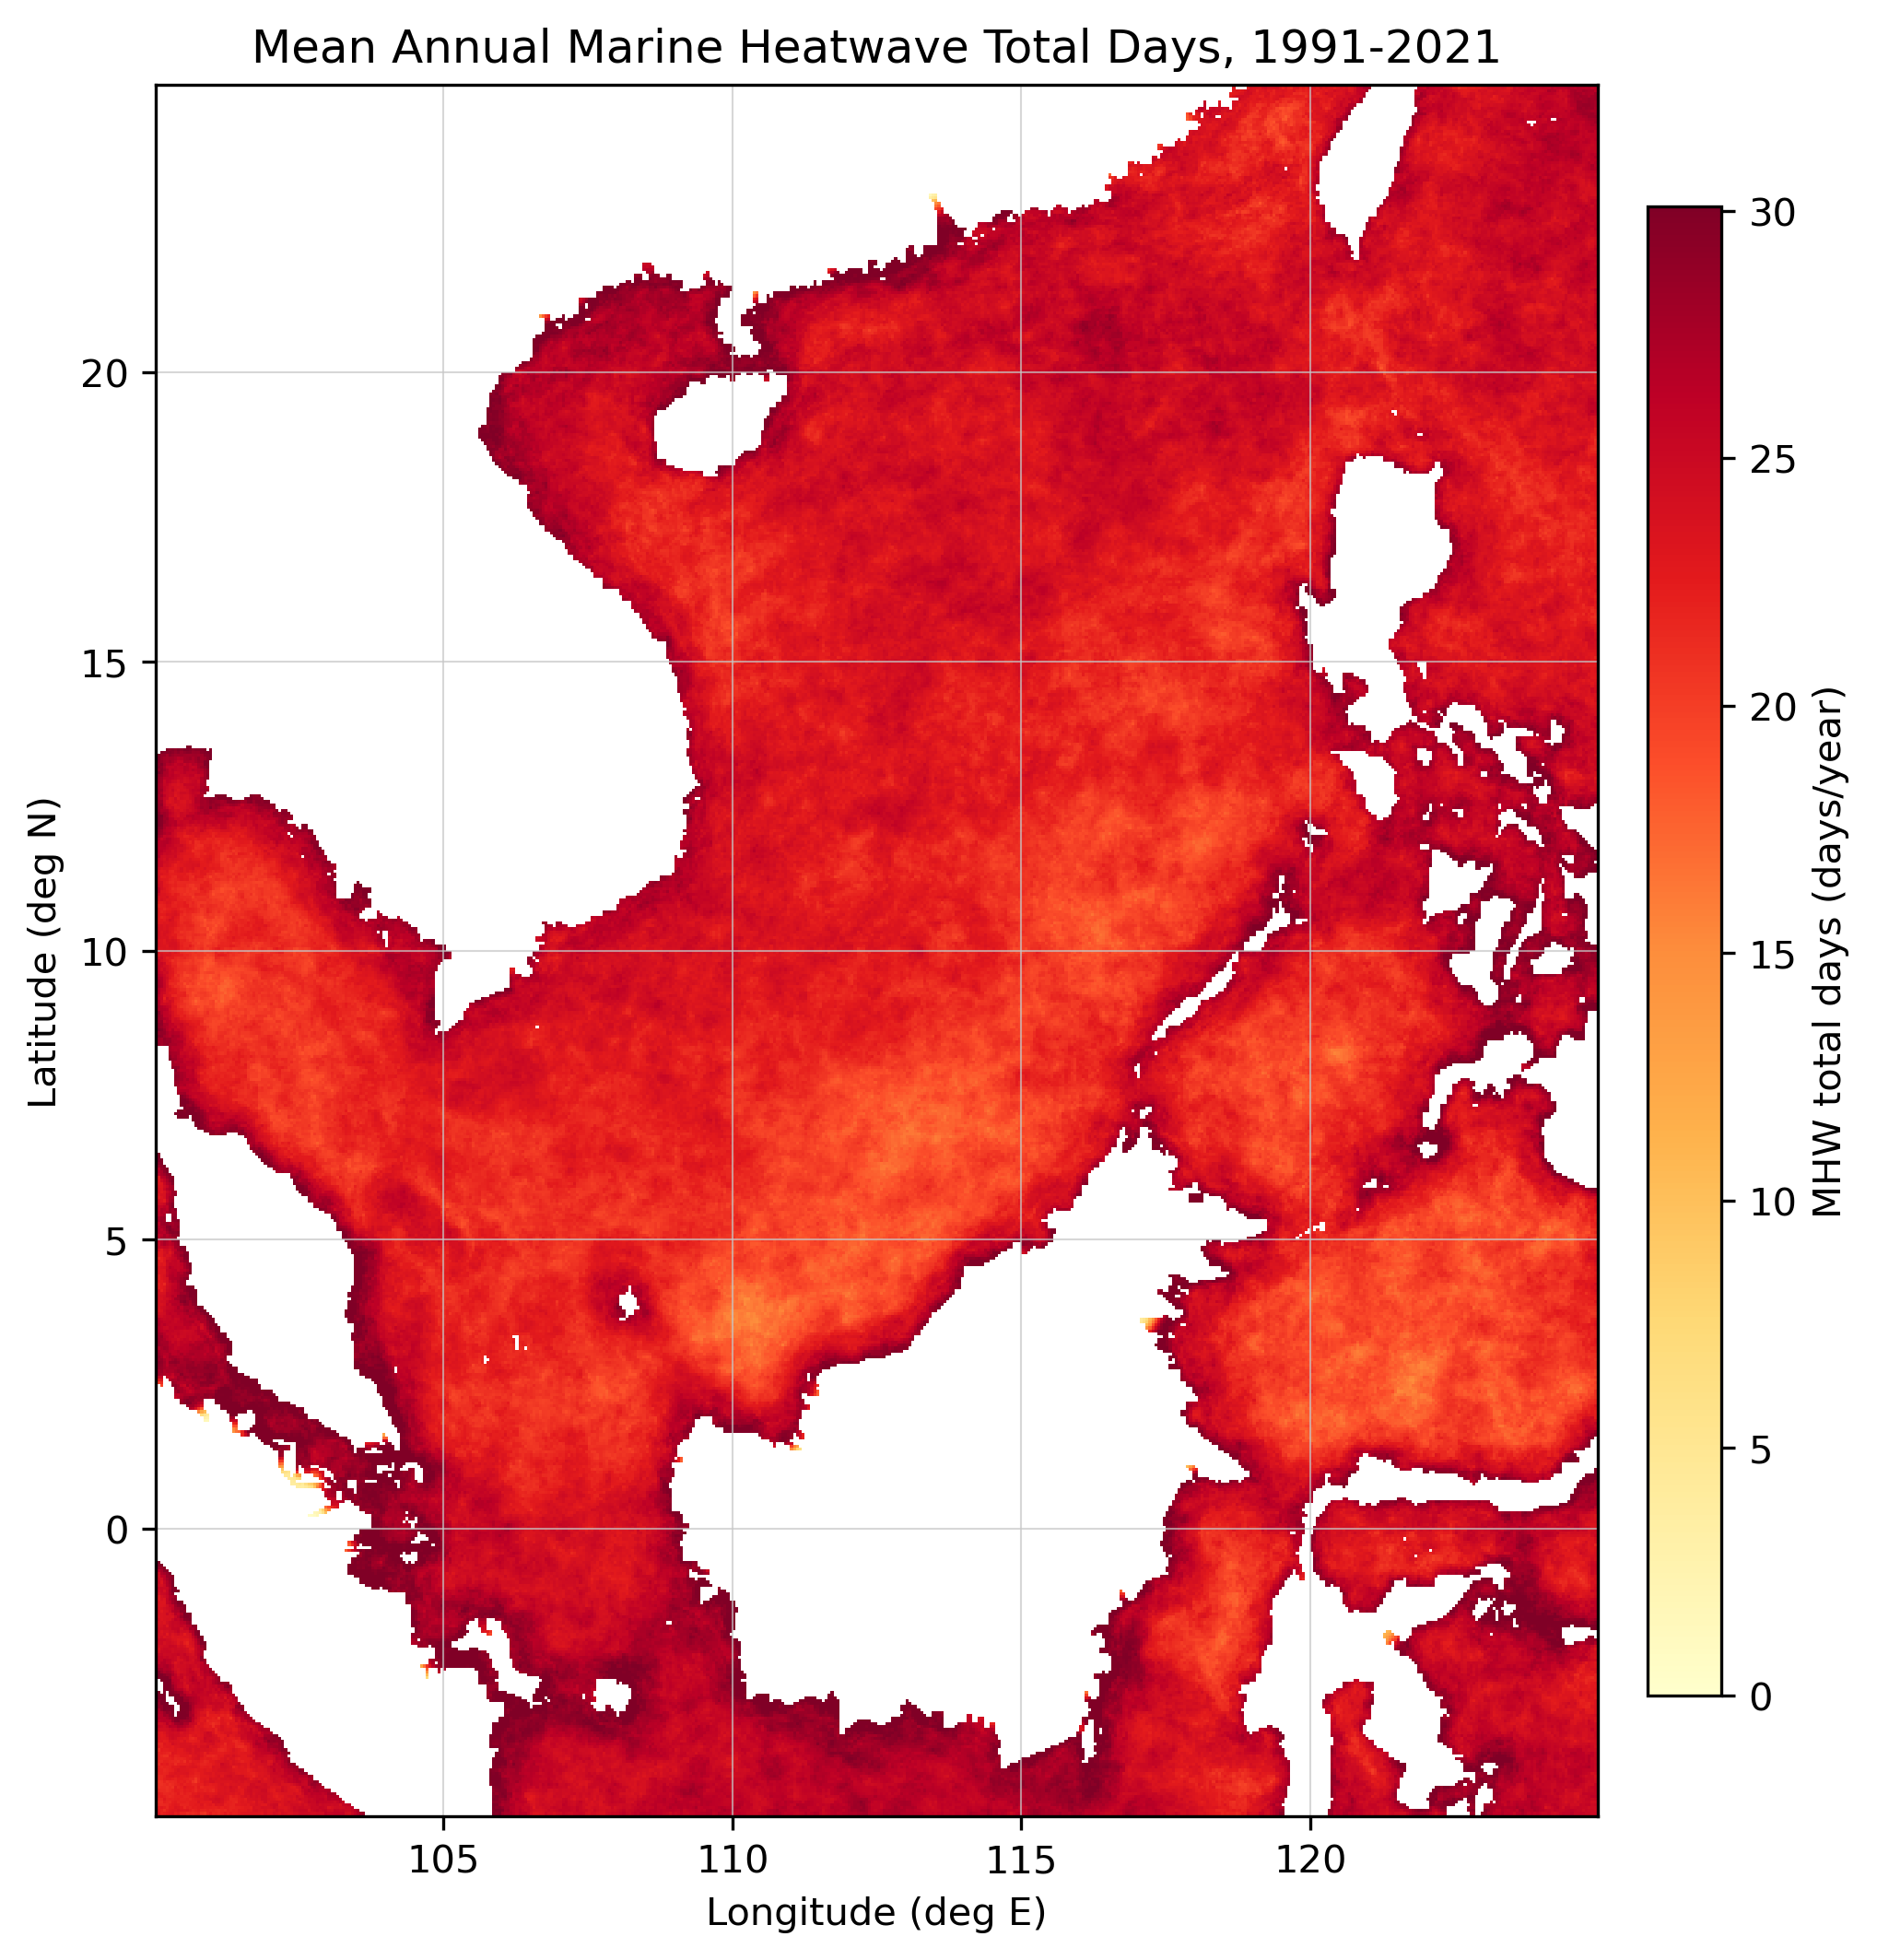
\includegraphics[width=\textwidth]{mhw_mean_total_days_map.png}
\caption{多年平均 MHW 总天数}
\end{subfigure}
\hfill
\begin{subfigure}{0.48\textwidth}
\centering
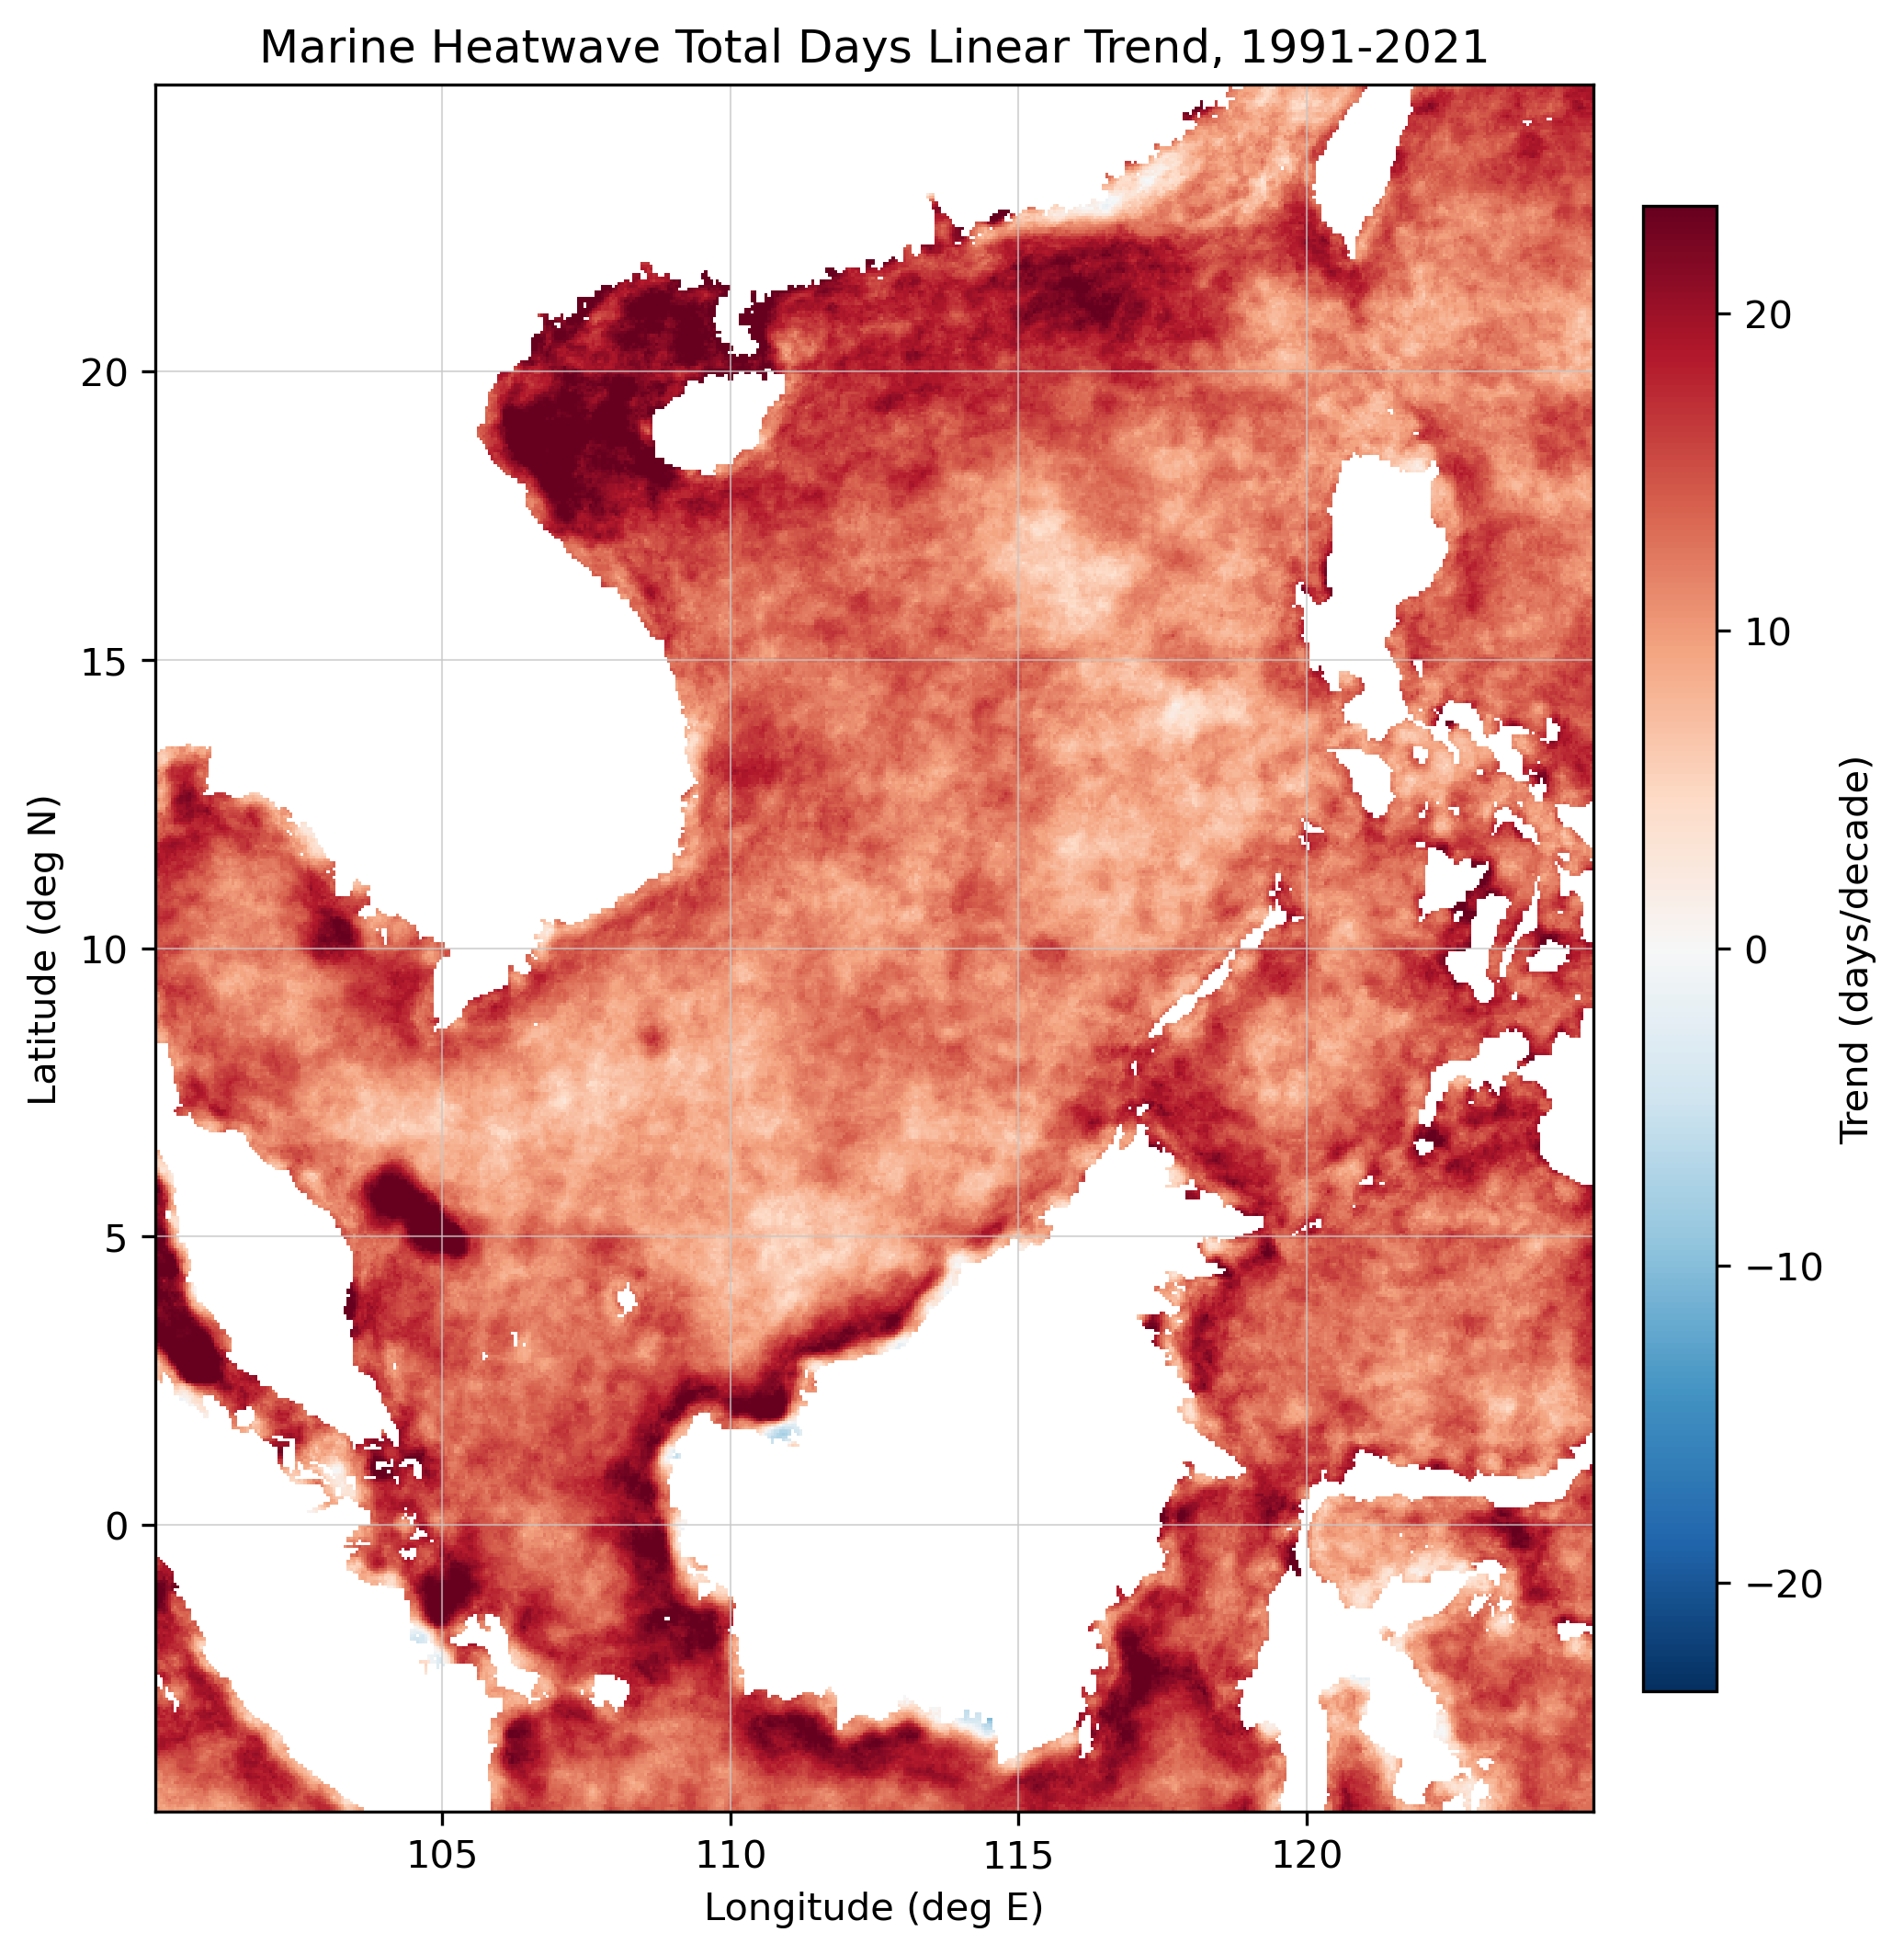
\includegraphics[width=\textwidth]{mhw_total_days_trend_map.png}
\caption{MHW 总天数趋势}
\end{subfigure}
\caption{南海年度 MHW 总天数空间格局及趋势}
\end{figure}

\begin{figure}[H]
\centering
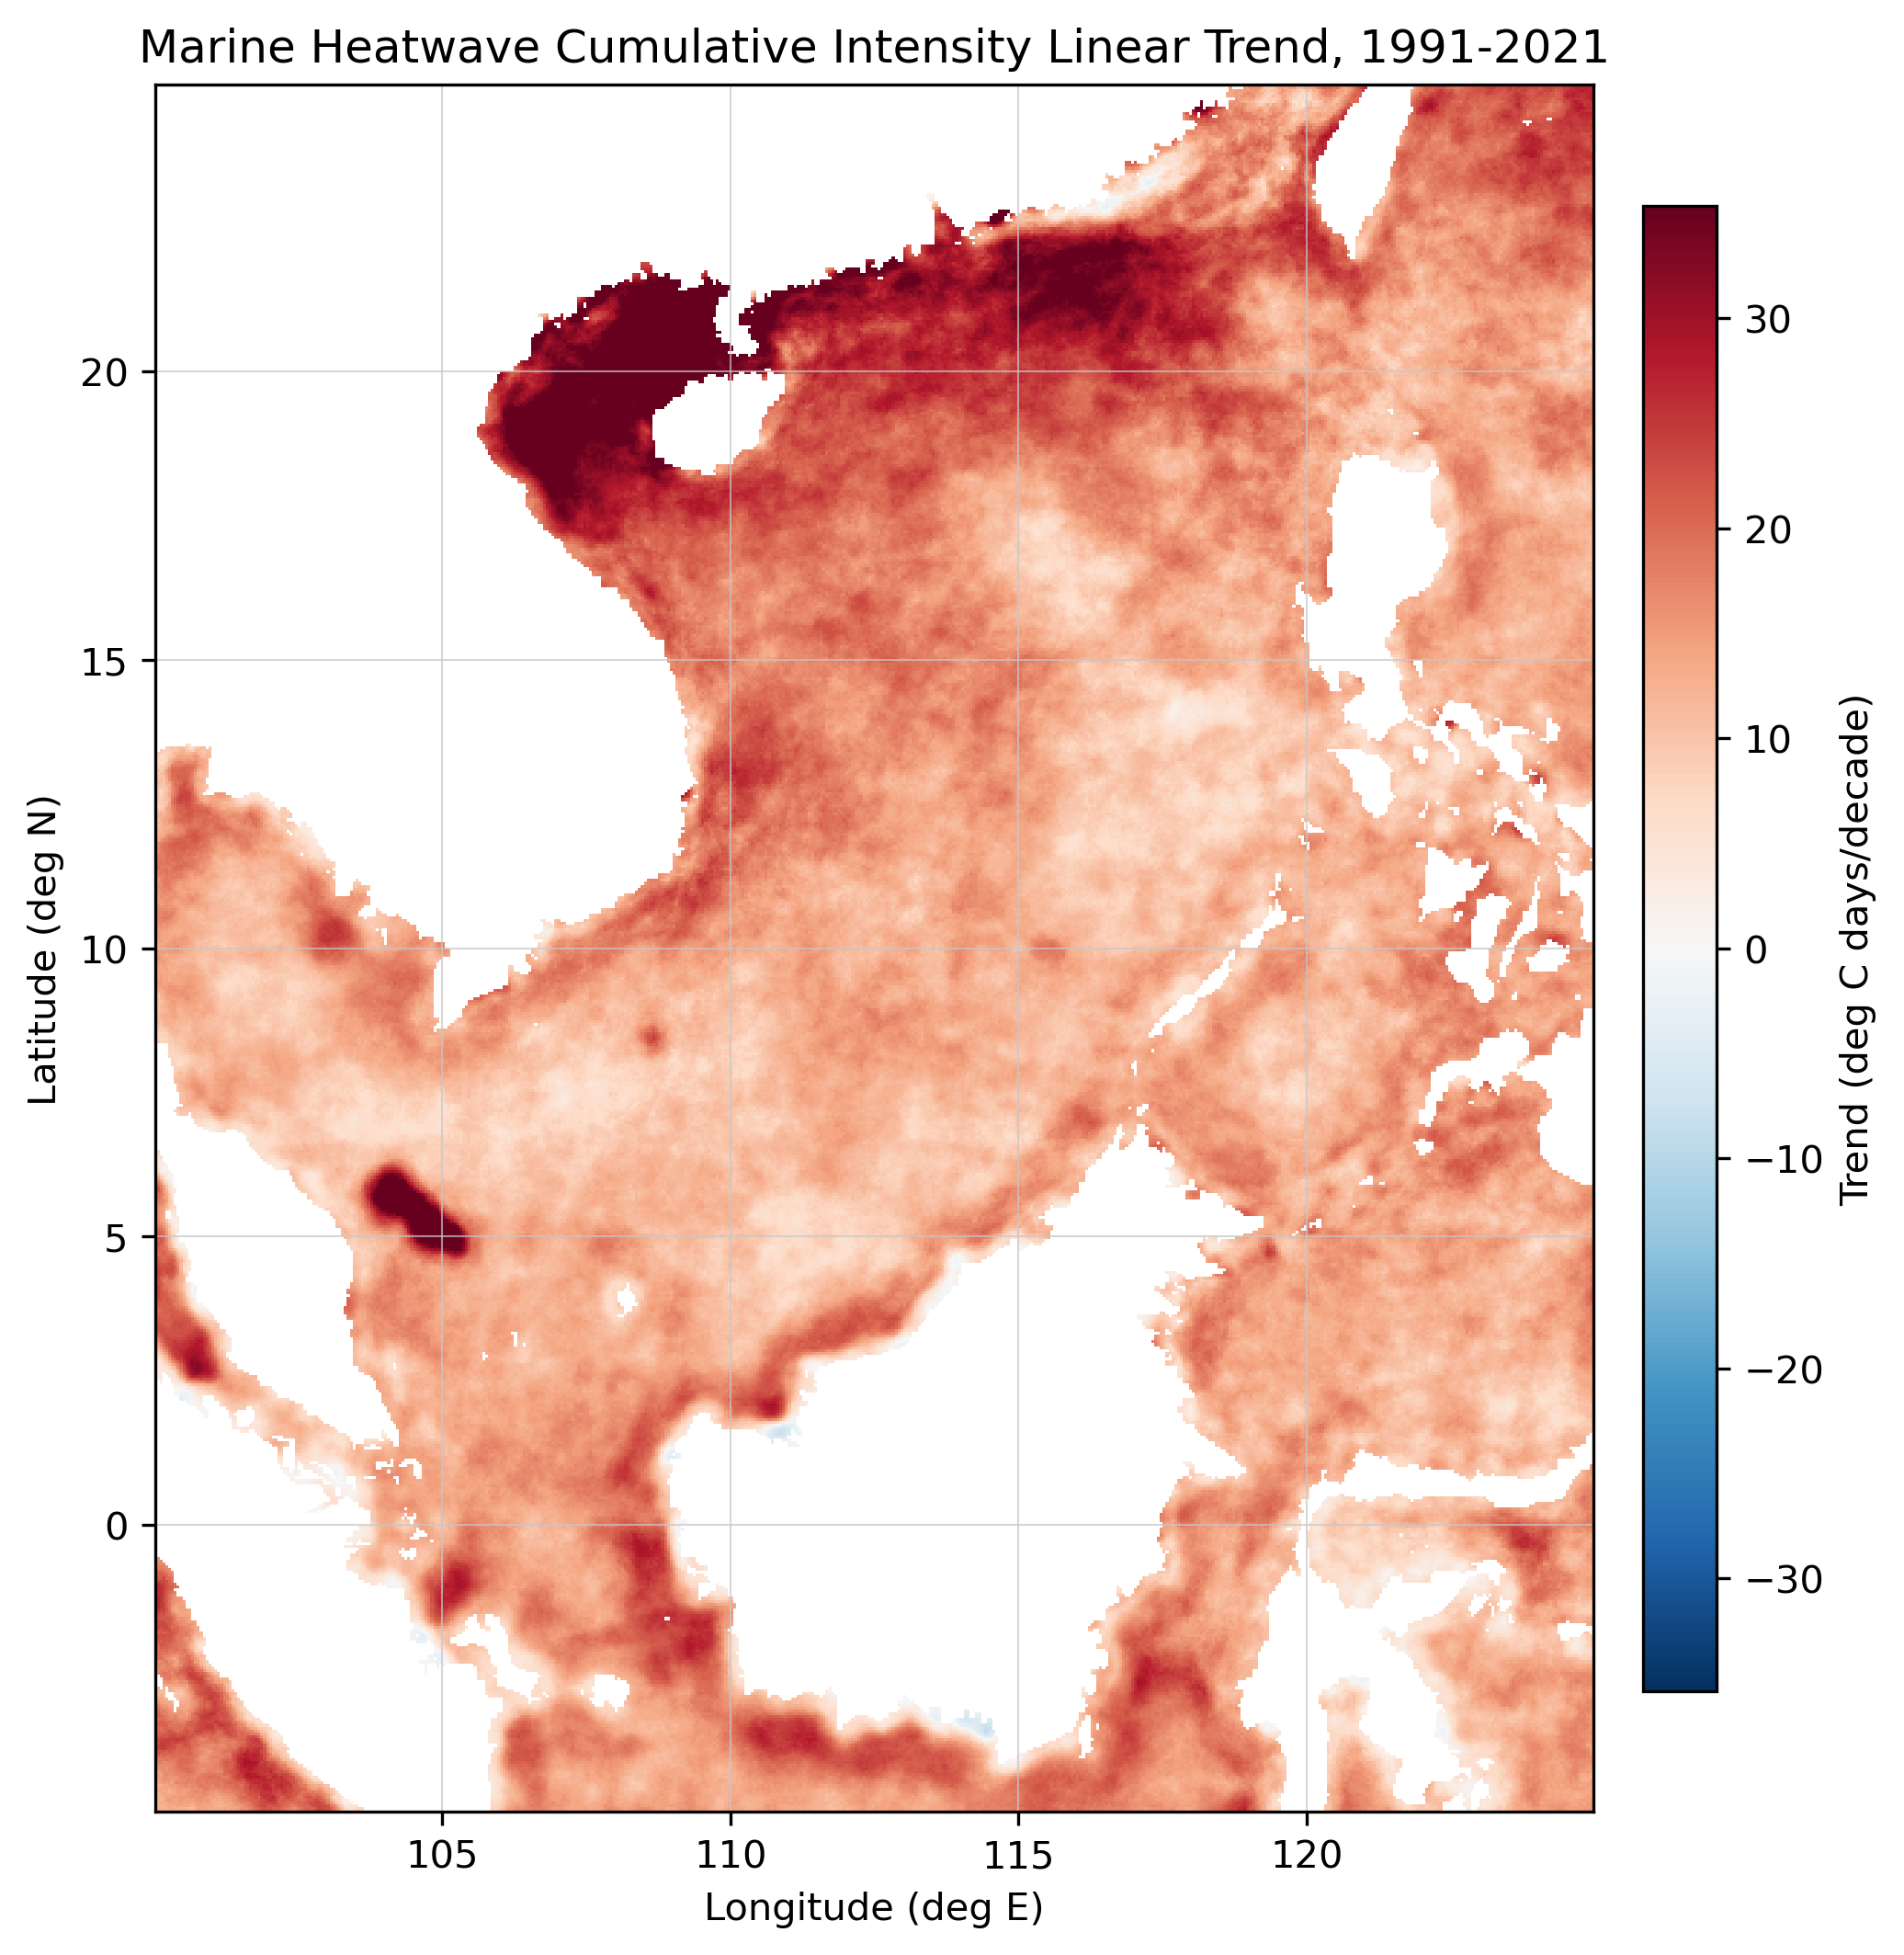
\includegraphics[width=0.76\textwidth]{mhw_cumulative_intensity_trend_map.png}
\caption{南海年度 MHW 累计强度趋势空间分布}
\end{figure}

\subsection{阈值敏感性检验说明结论稳健}
MHW 的绝对事件数量会随阈值变化，因此本文比较 85\%、90\% 和 95\% 三种分位阈值。表 5 和图 10 显示，阈值越高，平均频次和平均总天数越低，这是事件定义收紧后的自然结果；但三种阈值下 MHW 总天数趋势和累计强度趋势均保持正向。85\% 阈值下总天数趋势为 $21.749$ 天/10年，90\% 阈值下为 $13.381$ 天/10年，95\% 阈值下仍为 $5.286$ 天/10年。该结果说明，南海热浪风险增强并不依赖单一 90\% 阈值设定。

\begin{table}[H]
\centering
\caption{MHW 阈值敏感性检验}
\resizebox{\textwidth}{!}{\begin{tabular}{lccccc}
\hline
阈值 & 平均频次 & 平均总天数 & 总天数趋势 & 累计强度趋势 & 结论是否一致 \\
 & (次/年) & (天/年) & (天/10年) & ($^\circ$C$\cdot$天/10年) & \\
\hline
85\% & 3.778 & 39.838 & 21.749 & 21.855 & 一致 \\
90\% & 2.522 & 23.575 & 13.381 & 15.176 & 一致 \\
95\% & 1.185 & 9.294 & 5.286 & 7.073 & 一致 \\
\hline
\end{tabular}
}
\end{table}

\begin{figure}[H]
\centering
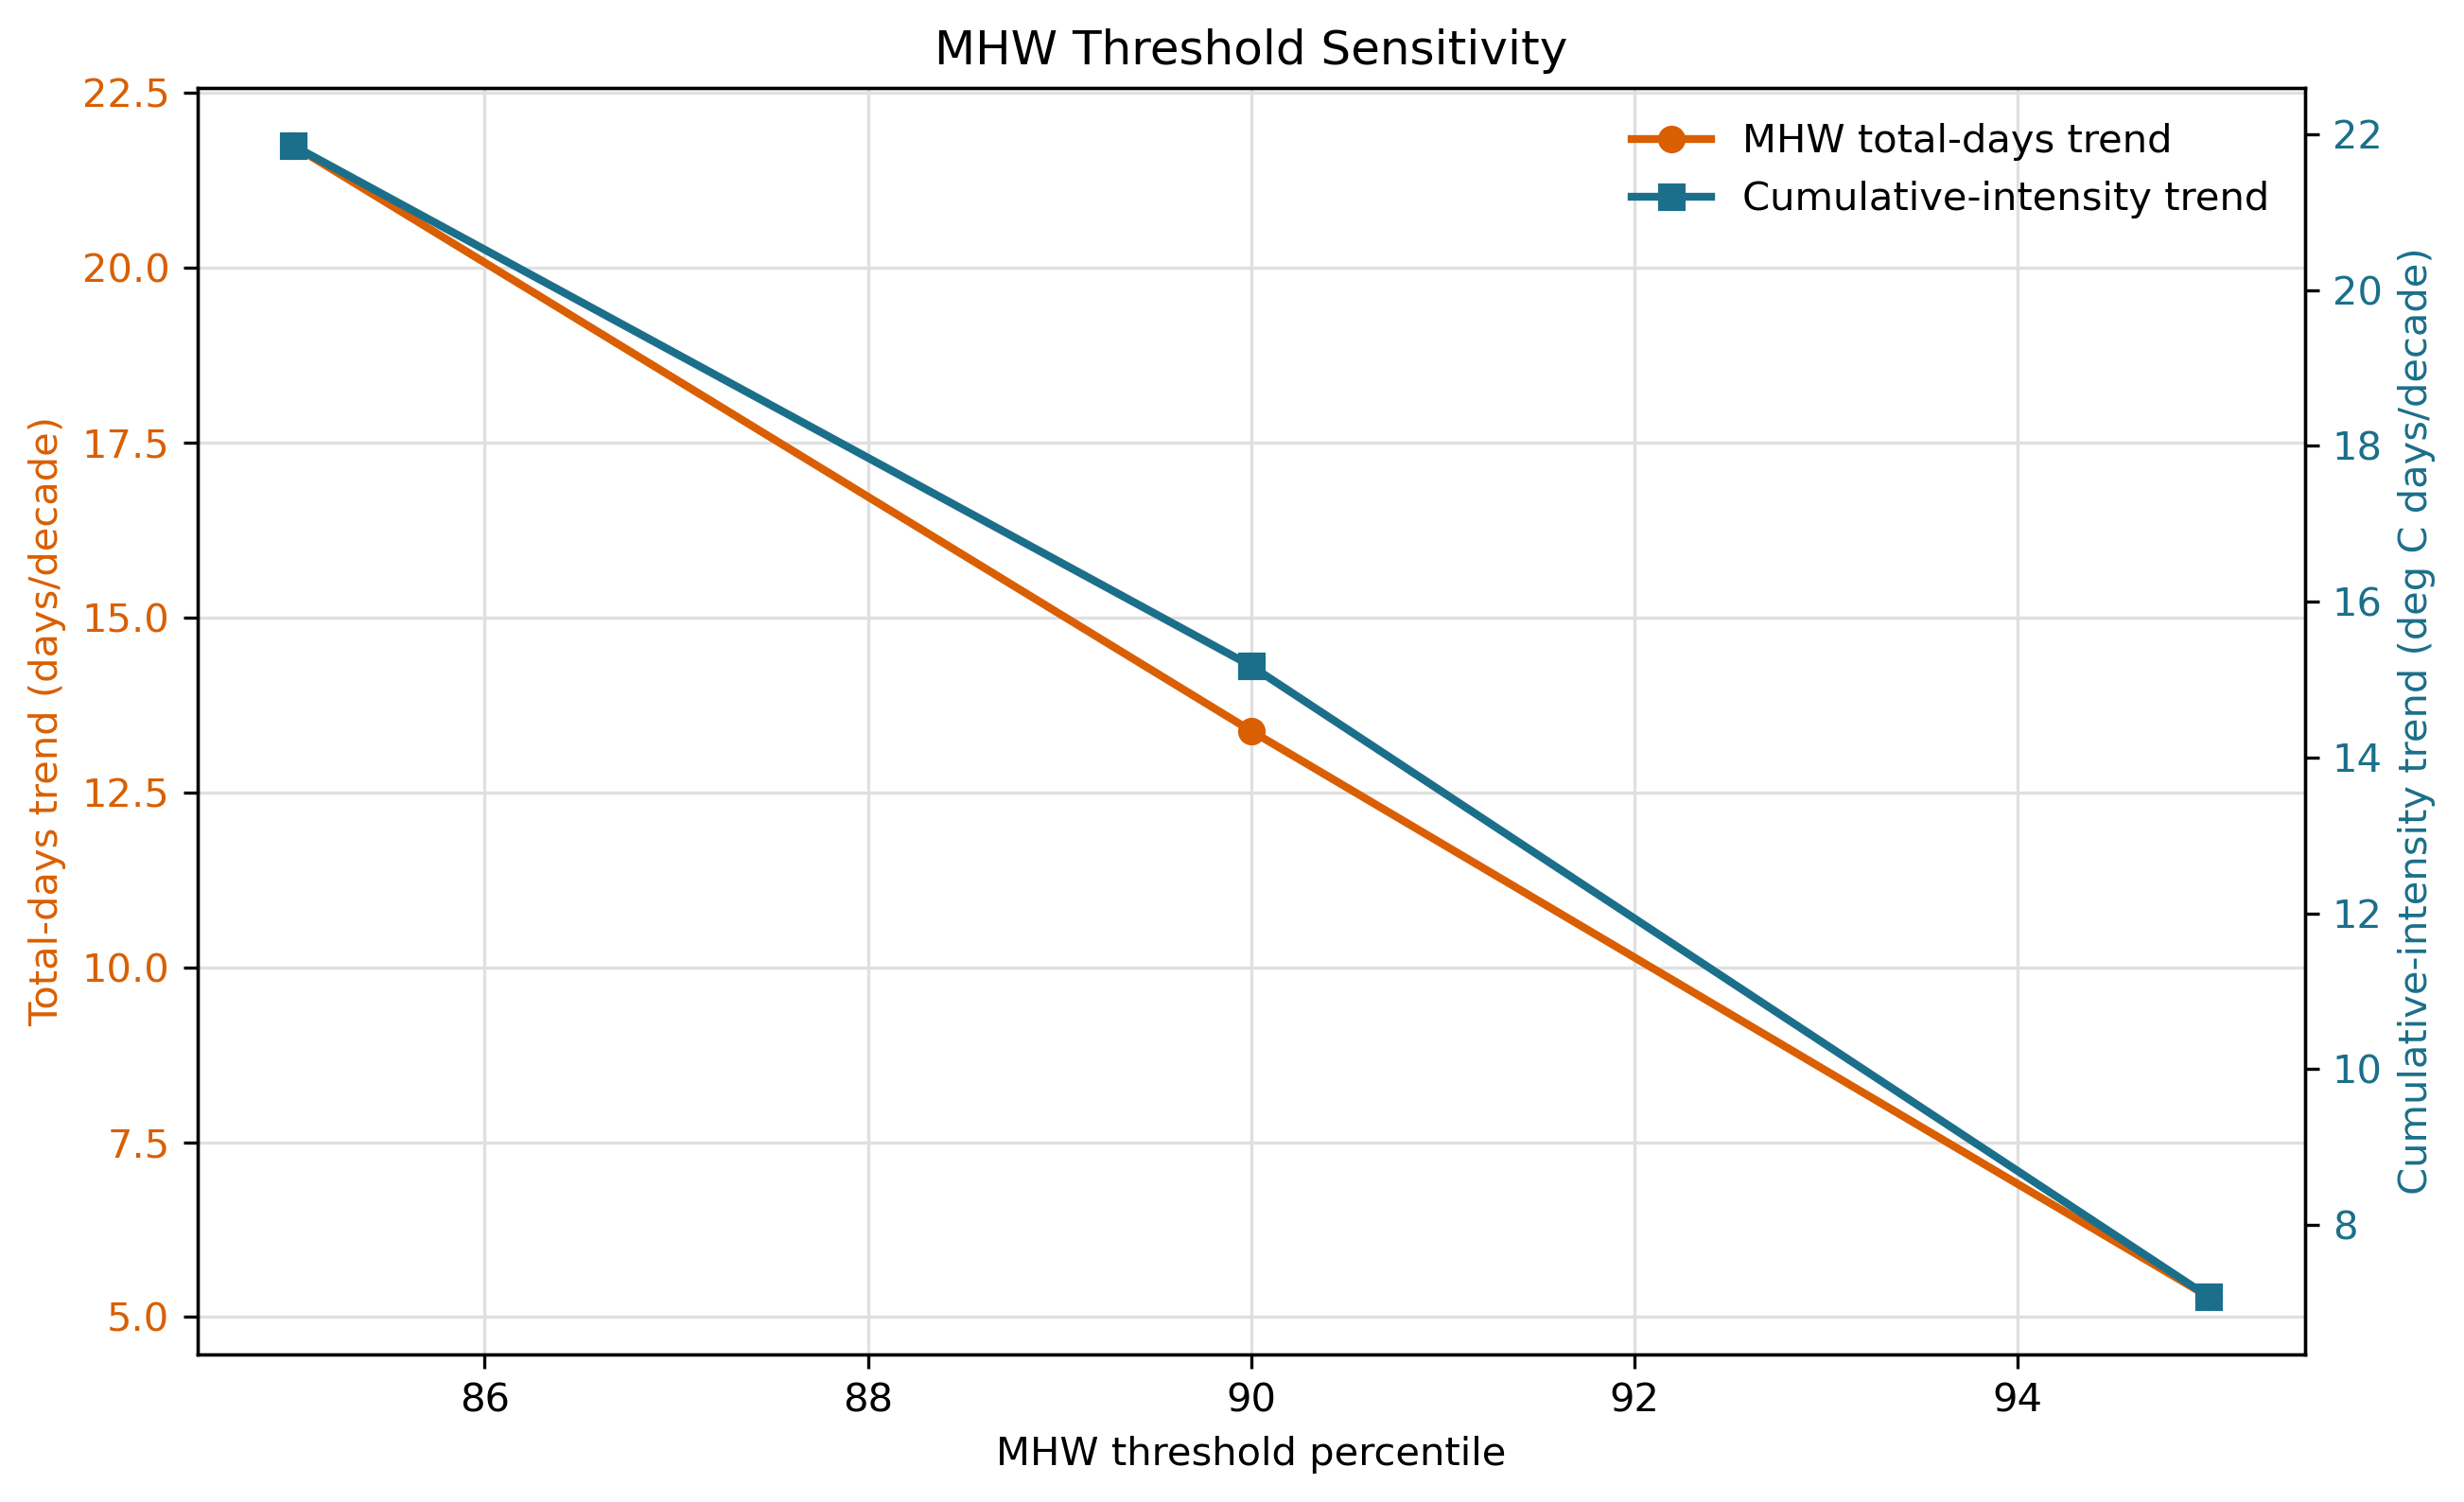
\includegraphics[width=0.78\textwidth]{mhw_threshold_sensitivity.png}
\caption{不同阈值下 MHW 总天数与累计强度趋势}
\end{figure}

\subsection{综合热风险指数识别重点海区}
为综合平均态增暖和海洋热浪暴露，本文构建相对综合海洋热风险指数 HRI。图 11 给出了 HRI 空间分布，表 6 汇总分区结果。北部陆架平均 HRI 为 0.574，高风险格点占比为 16.6\%，在五个统计分区中最高；西部近岸平均 HRI 为 0.537，高风险格点占比为 13.5\%。各分区的主导风险来源均为热浪暴露均值，说明长期高温暴露背景是当前综合风险排序中的关键分量。HRI 并不表示生态损失概率，但能够为监测布点和风险优先级提供统计依据。

\begin{table}[H]
\centering
\caption{南海分区相对综合海洋热风险指数}
\resizebox{\textwidth}{!}{\begin{tabular}{lcccc}
\hline
分区 & 平均HRI & 高风险格点占比 & 主导风险来源 & 应用含义 \\
\hline
北部陆架 & 0.574 & 16.6\% & 热浪暴露均值 & 重点跟踪 \\
中部海盆 & 0.505 & 0.0\% & 热浪暴露均值 & 重点跟踪 \\
南部南海 & 0.522 & 4.3\% & 热浪暴露均值 & 重点跟踪 \\
西部近岸 & 0.537 & 13.5\% & 热浪暴露均值 & 重点跟踪 \\
东部外海 & 0.528 & 3.2\% & 热浪暴露均值 & 重点跟踪 \\
\hline
\end{tabular}
}
\end{table}

\begin{figure}[H]
\centering
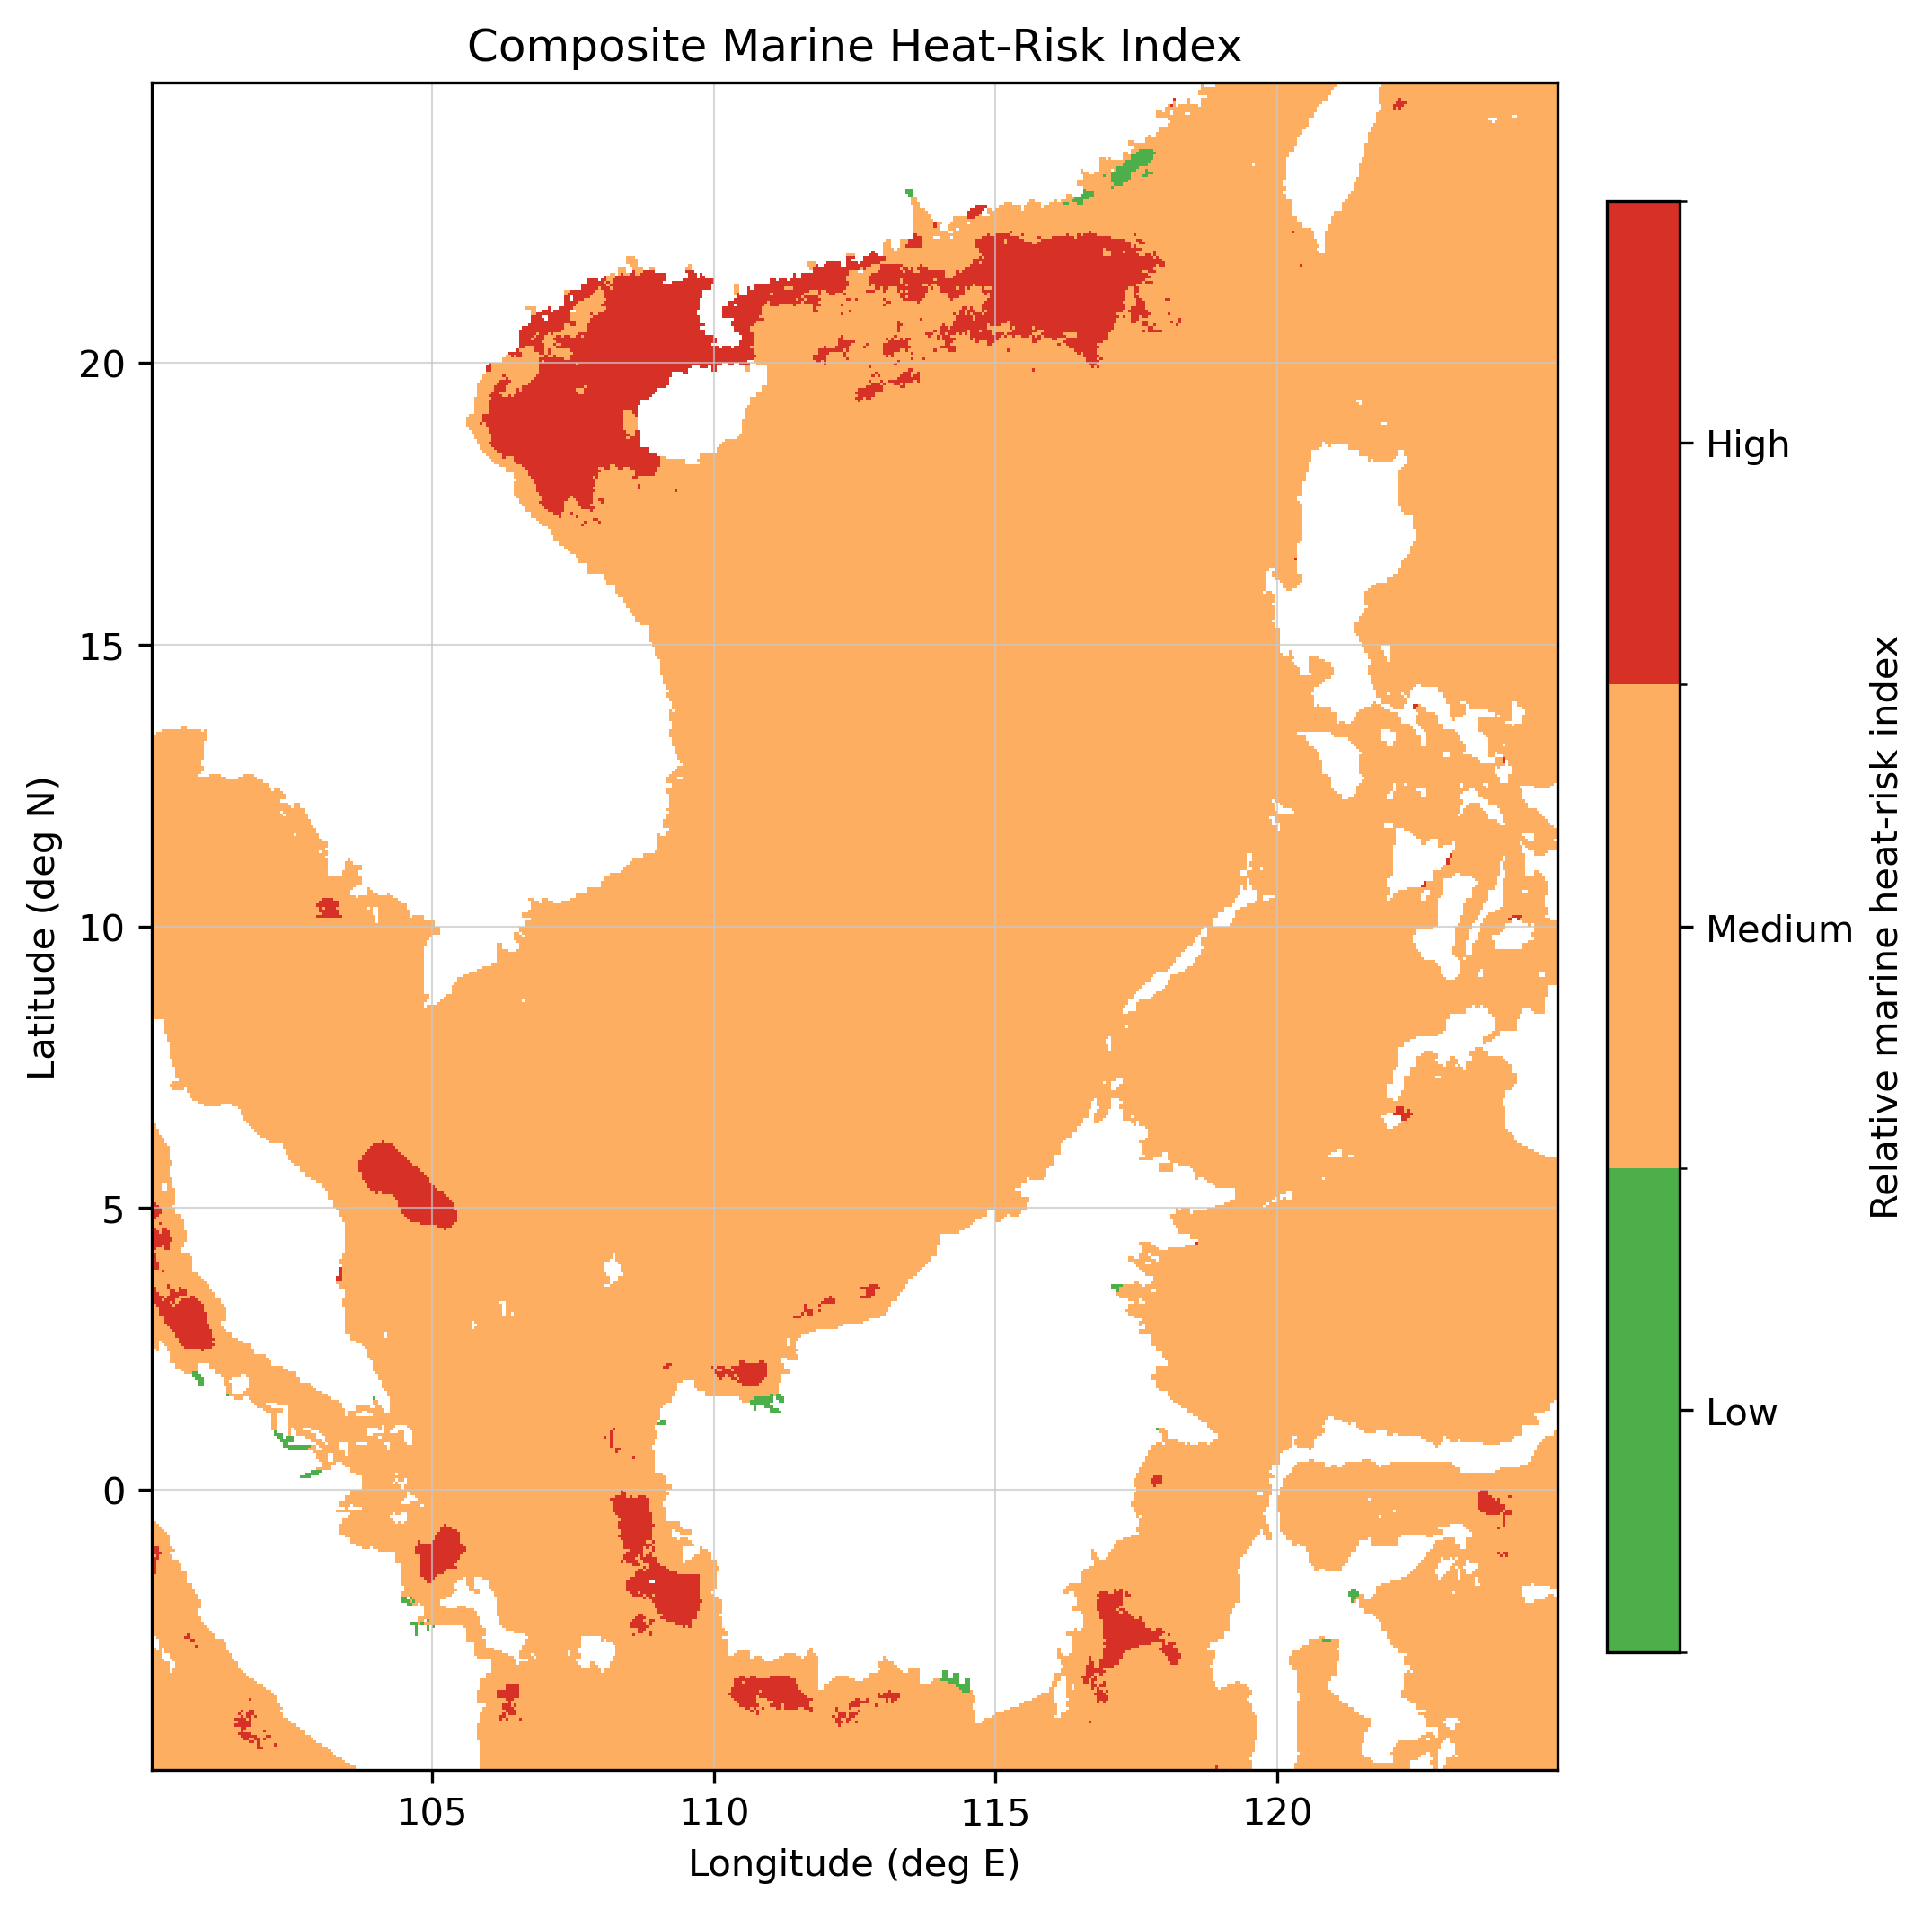
\includegraphics[width=0.78\textwidth]{heat_risk_index_map.png}
\caption{南海相对综合海洋热风险指数空间分布}
\end{figure}

本节结果表明，南海热风险已经从平均态增暖进一步表现为持续性高温事件增强。阈值敏感性和 HRI 结果共同说明，热风险增强具有稳定统计信号和明确空间优先区。

\section{气候驱动因子解释模型}

\subsection{滞后相关揭示月尺度响应关系}
表 7 汇总月尺度 SSTA 与主要驱动因子的最强滞后相关。风速距平与 SSTA 的同期相关最强，相关系数为 $-0.380$，且显著性水平较高。DMI 和 Niño 3.4 在 6 个月滞后下表现出正相关，说明印度洋偶极子和 ENSO 信号可能通过背景环流或遥相关影响南海热状态，但其相关强度低于风速距平。

\begin{table}[H]
\centering
\caption{月尺度 SSTA 与驱动因子的最强滞后相关}
\resizebox{\textwidth}{!}{\begin{tabular}{lcccc}
\hline
驱动因子 & 滞后/月 & $r$ & $p$ 值 & $n$ \\
\hline
wind\_speed\_anom & 0 & -0.380 & 4.20e-14 & 369 \\
dmi & 6 & 0.334 & 6.75e-11 & 363 \\
nino34\_cpc\_3m\_centered & 6 & 0.303 & 3.78e-09 & 363 \\
soi & 0 & 0.180 & 5.22e-04 & 369 \\
wind\_speed & 0 & -0.162 & 0.002 & 369 \\
pdo & 0 & -0.107 & 0.040 & 369 \\
\hline
\end{tabular}
}
\end{table}

\subsection{标准化回归比较边际解释强度}
月尺度 SSTA 标准化解释模型见表 8。模型调整 $R^2$ 为 0.215，说明所选驱动因子能够解释约五分之一的月尺度 SSTA 标准化波动。Niño 3.4（滞后 3 月）和风速距平均通过显著性检验，其中风速距平系数为 $-0.363$，是稳定的负向解释变量；PDO 系数为 $-0.273$，DMI 在多元模型中未达到显著水平。

\begin{table}[H]
\centering
\caption{月尺度 SSTA 标准化解释模型}
\resizebox{\textwidth}{!}{\begin{tabular}{lcccc}
\hline
变量 & 标准化系数 & $t$ & $p$ 值 & VIF \\
\hline
截距 & -6.96e-17 & -1.50e-15 & 1.000 & -- \\
Ni\~{n}o 3.4（滞后3月） & 0.320 & 5.688 & 2.66e-08 & 1.473 \\
PDO（同期） & -0.273 & -4.874 & 1.64e-06 & 1.462 \\
DMI（同期） & -0.045 & -0.945 & 0.345 & 1.075 \\
风速距平（同期） & -0.363 & -7.770 & 8.24e-14 & 1.012 \\
\hline
\end{tabular}
}
\end{table}

年度 MHW 总天数解释模型见表 9 和表 10。模型调整 $R^2$ 为 0.206，风速距平标准化系数为 $-0.558$，$p=0.003$，说明风速偏弱年份更容易对应更长的 MHW 暴露时长。其他大尺度气候指数在年度样本下未通过显著性检验，表明其影响可能更多体现为季节性、区域性或非线性调制。

\begin{table}[H]
\centering
\caption{年度 MHW 总天数标准化解释模型}
\resizebox{\textwidth}{!}{\begin{tabular}{lcccc}
\hline
变量 & 标准化系数 & $t$ & $p$ 值 & VIF \\
\hline
截距 & 0.000 & 0.000 & 1.000 & -- \\
Ni\~{n}o 3.4 & 0.083 & 0.327 & 0.747 & 2.425 \\
PDO & -0.150 & -0.591 & 0.560 & 2.430 \\
DMI & 0.171 & 0.892 & 0.381 & 1.382 \\
风速距平 & -0.558 & -3.266 & 0.003 & 1.102 \\
\hline
\end{tabular}
}
\end{table}

\begin{table}[H]
\centering
\caption{驱动因子解释模型拟合优度}
\resizebox{0.72\textwidth}{!}{\begin{tabular}{lccc}
\hline
模型 & $n$ & $R^2$ & 调整 $R^2$ \\
\hline
月尺度 SSTA 解释模型 & 366 & 0.224 & 0.215 \\
年度 MHW 总天数解释模型 & 31 & 0.312 & 0.206 \\
\hline
\end{tabular}
}
\end{table}

\subsection{局地风速异常的统计意义与物理解释}
图 12 展示驱动因子相关热图，图 13 展示月尺度 SSTA 和年度 MHW 总天数回归拟合。风速距平在相关分析和多元回归中均保持负向影响，说明其统计信号较为稳定。从物理含义上看，弱风条件可能降低潜热和感热释放，削弱上层海水混合，使近表层暖异常更容易维持并累积为持续高温暴露。需要强调的是，本文回归模型识别的是统计关联，而非单独证明因果机制。

\begin{figure}[H]
\centering
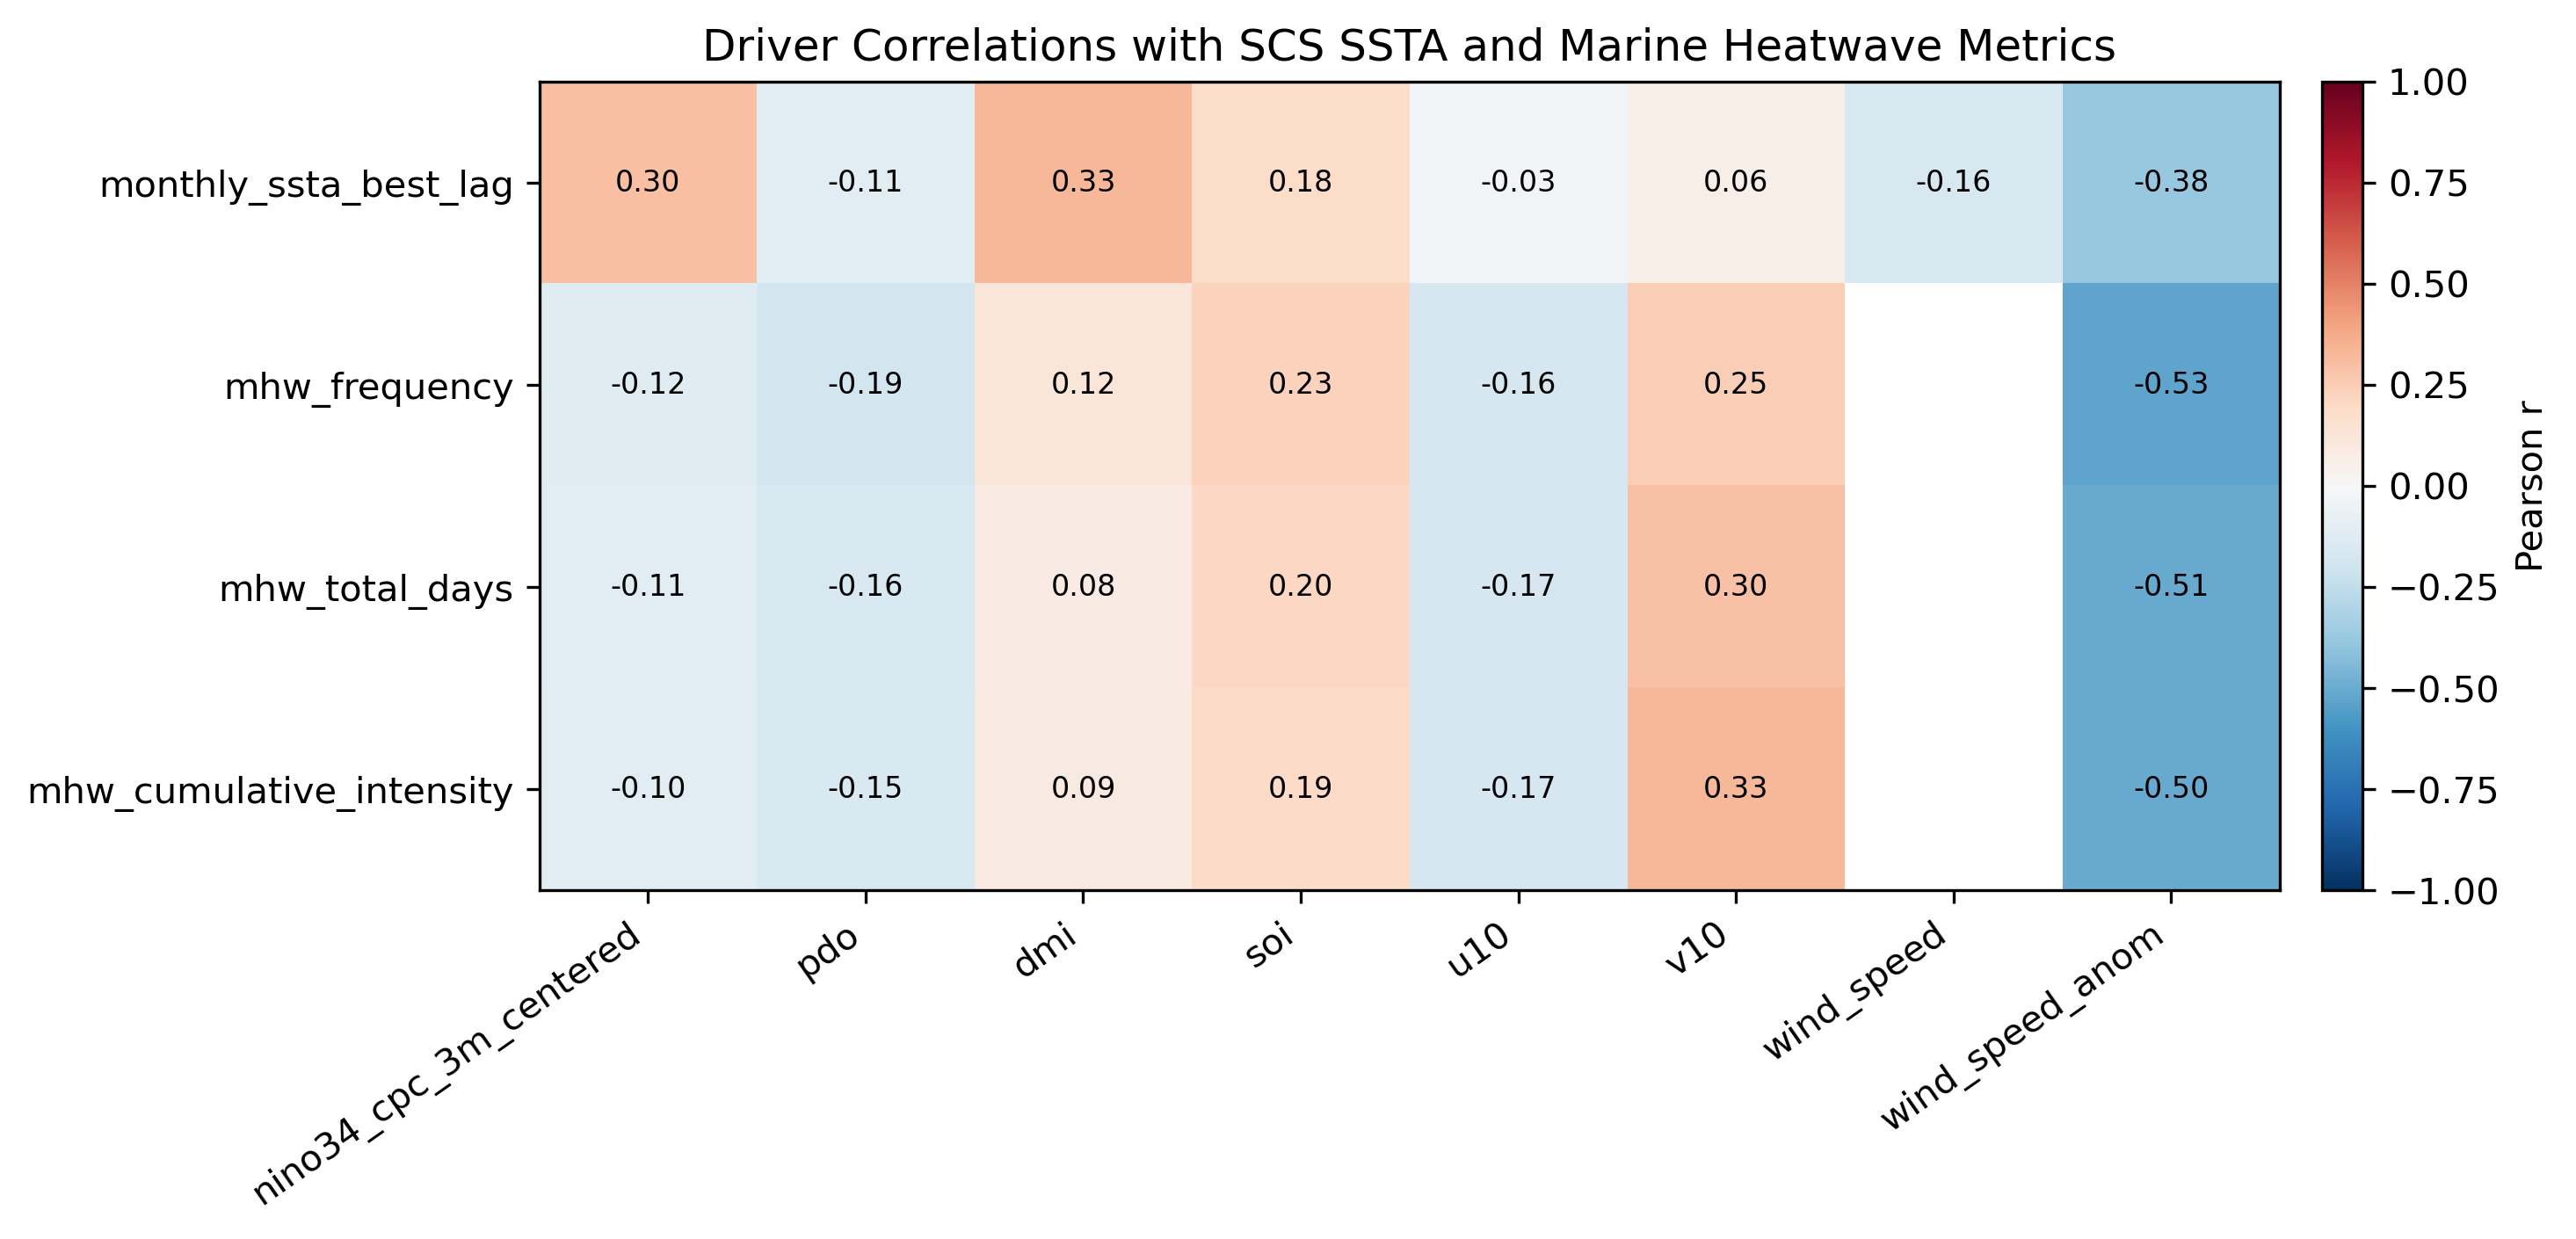
\includegraphics[width=\textwidth]{driver_correlation_heatmap.png}
\caption{南海 SSTA 与 MHW 指标的驱动因子相关热图}
\end{figure}

\begin{figure}[H]
\centering
\begin{subfigure}{0.48\textwidth}
\centering
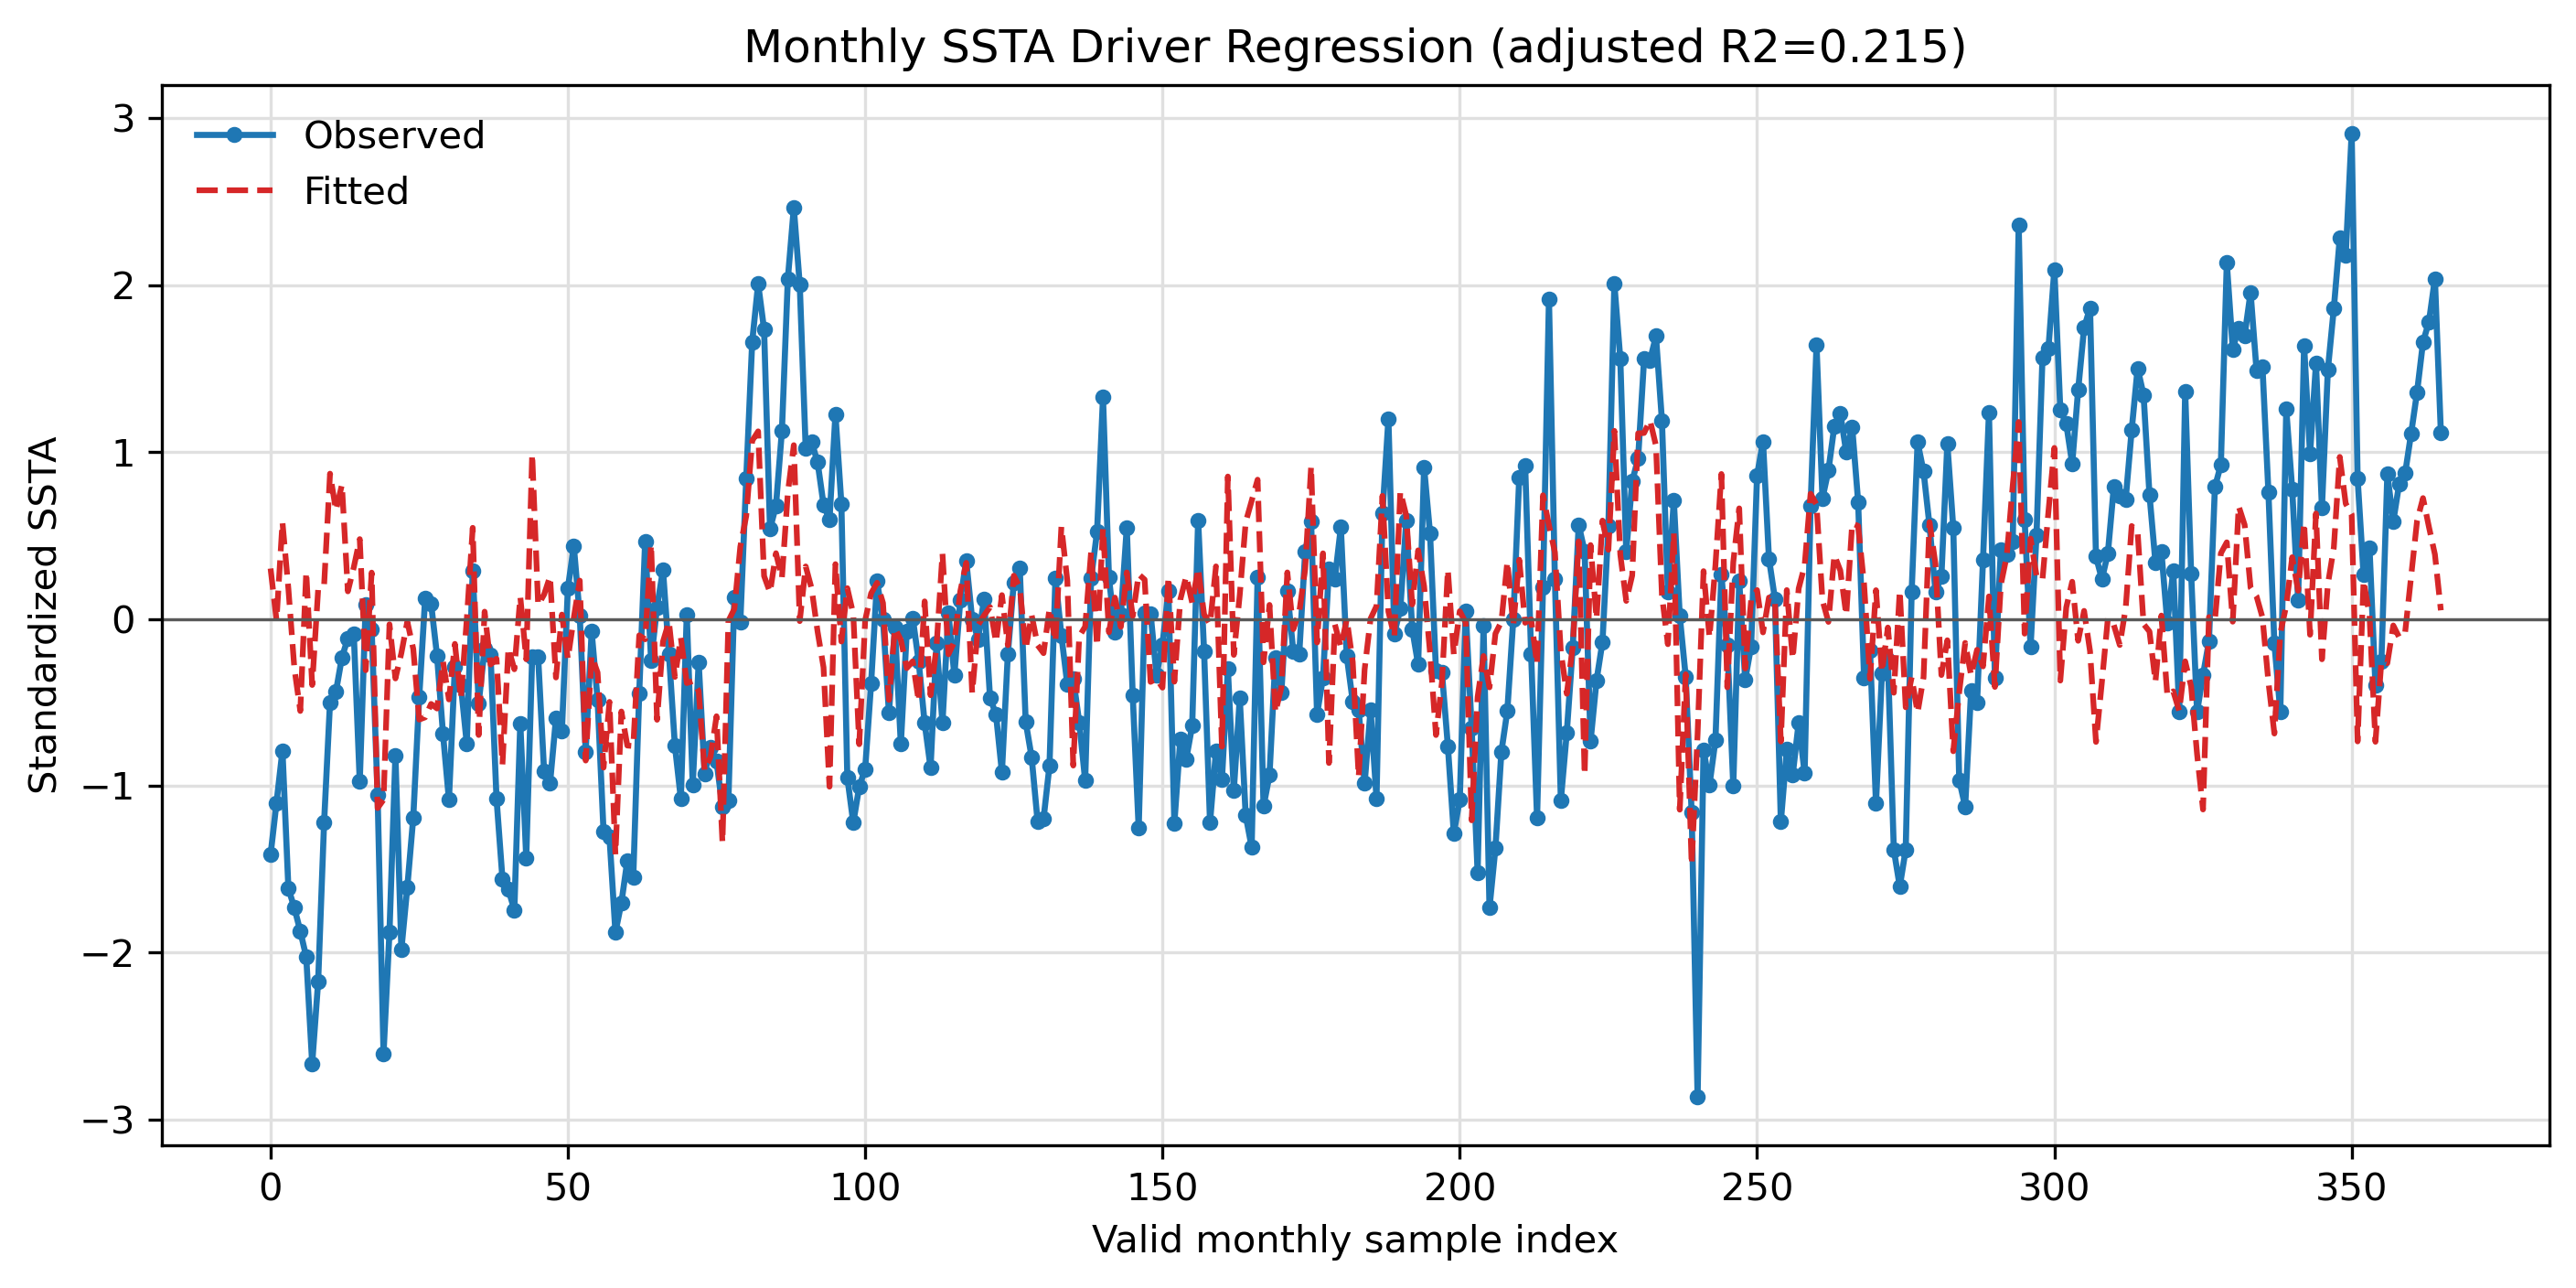
\includegraphics[width=\textwidth]{monthly_ssta_driver_fit.png}
\caption{月尺度 SSTA 回归拟合}
\end{subfigure}
\hfill
\begin{subfigure}{0.48\textwidth}
\centering
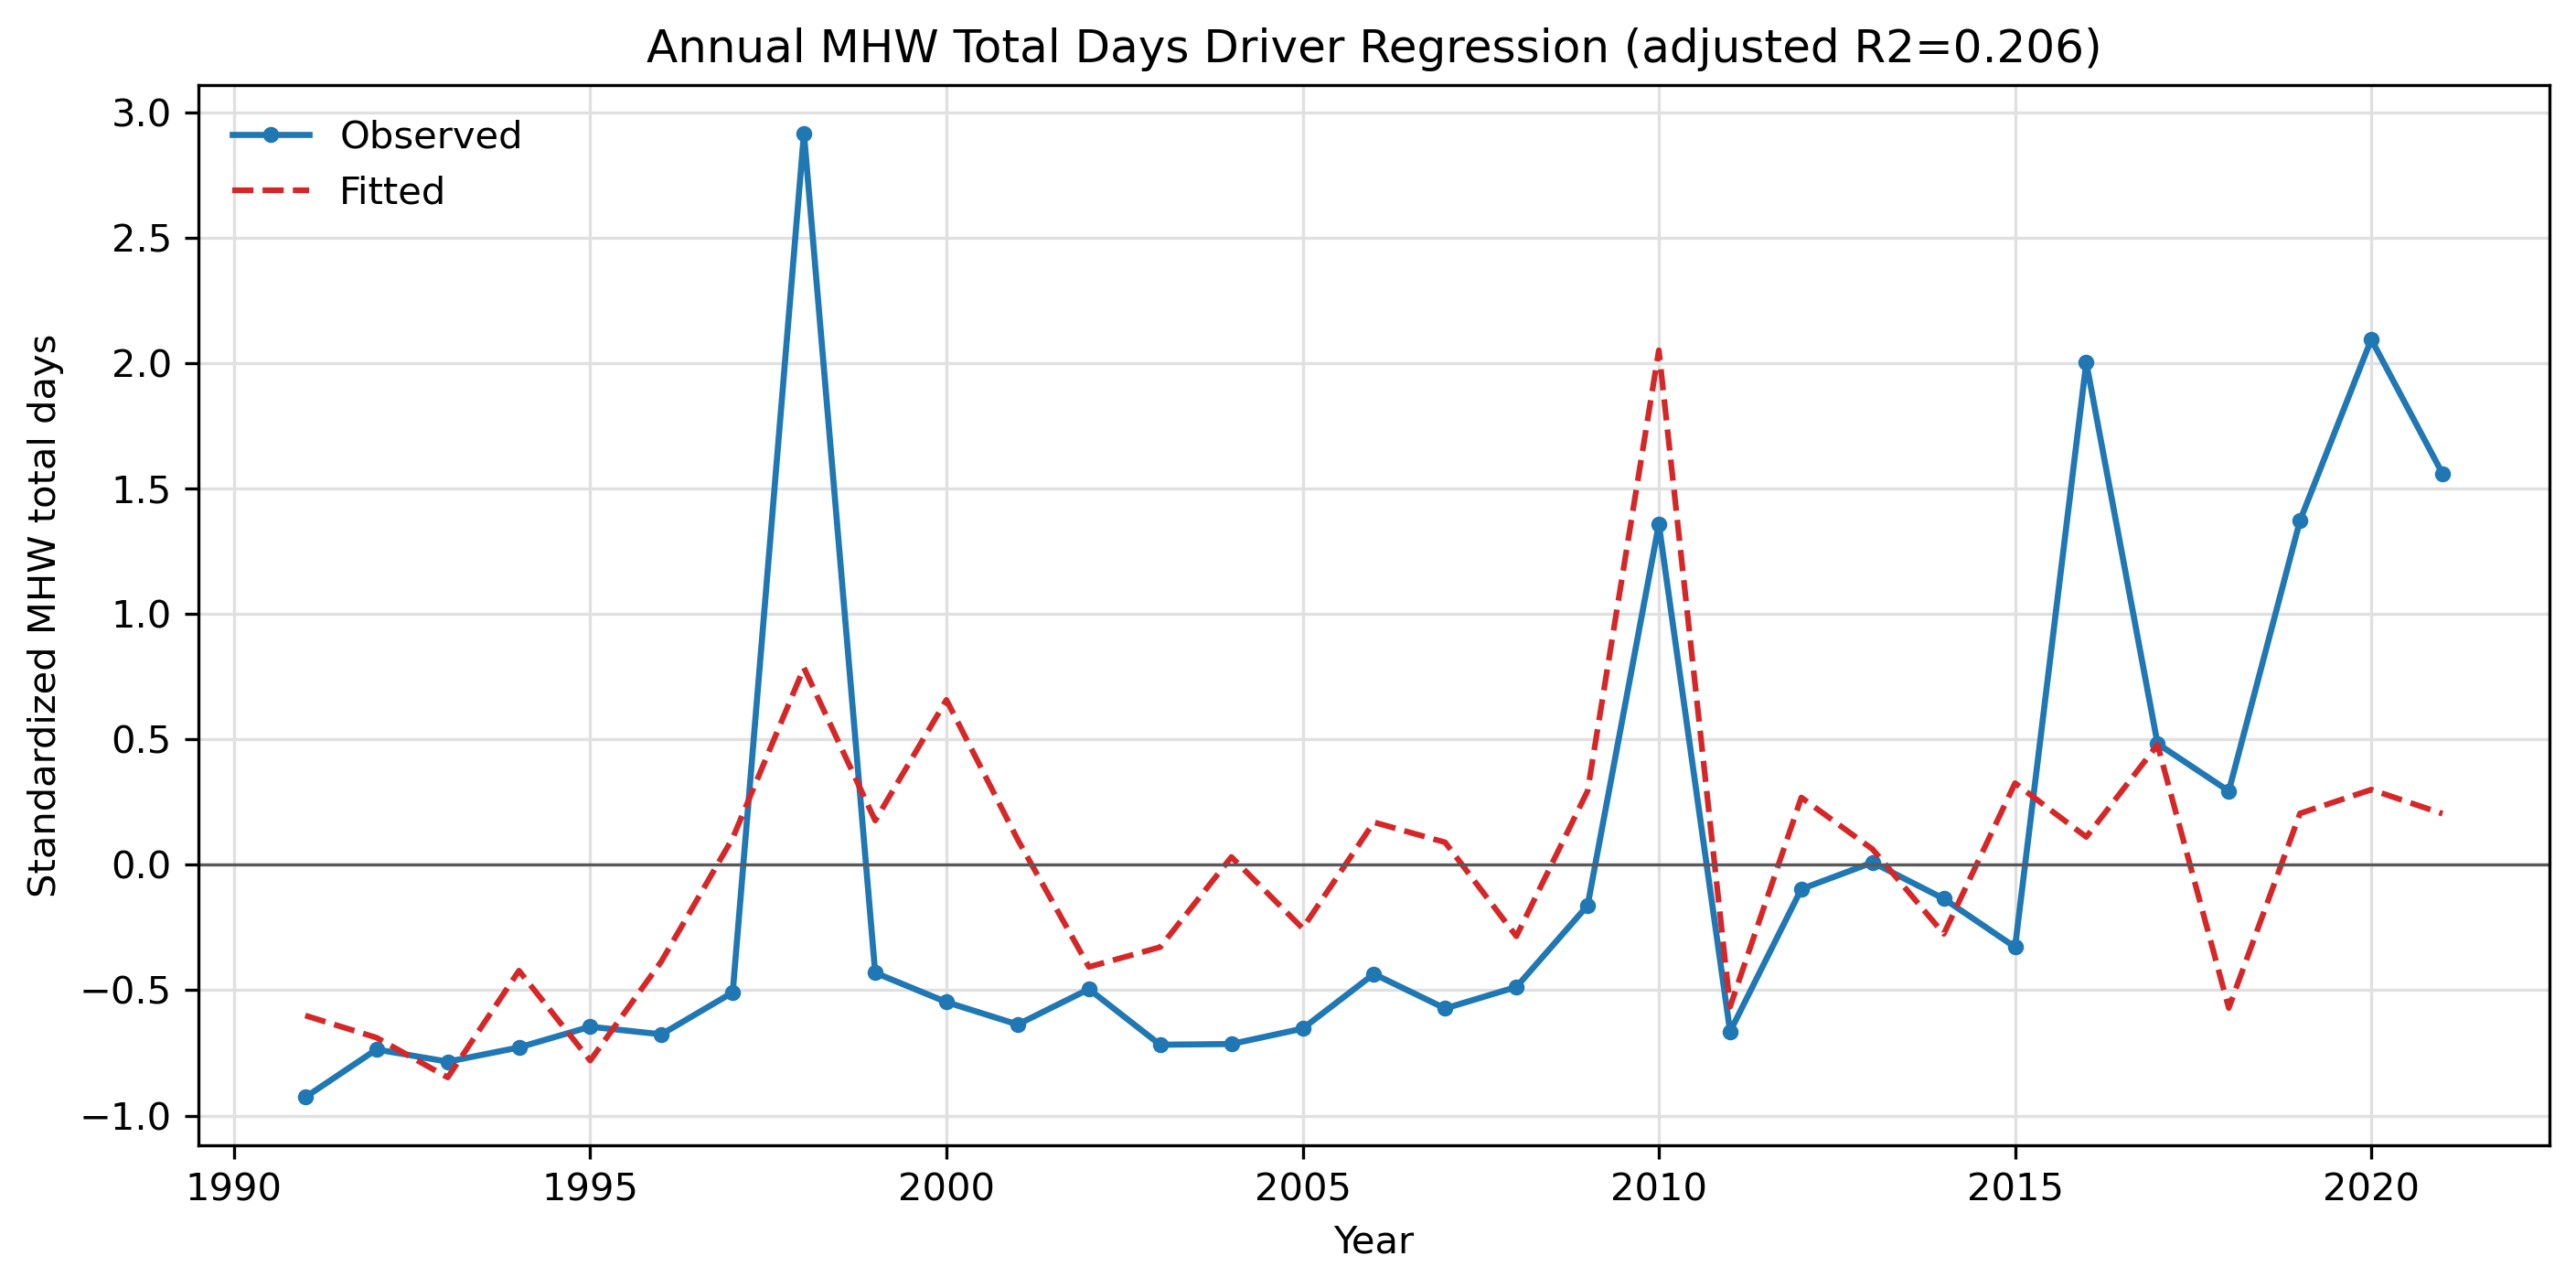
\includegraphics[width=\textwidth]{annual_mhw_driver_fit.png}
\caption{年度 MHW 总天数回归拟合}
\end{subfigure}
\caption{驱动因子标准化回归模型拟合结果}
\end{figure}

\subsection{大尺度气候指数的有限解释力}
ENSO、IOD 和 PDO 等大尺度气候信号能够影响西太平洋和印度洋背景环流，但本文年度 MHW 模型中这些变量并未表现出与风速距平同等稳定的解释力。这并不意味着大尺度信号无影响，而是说明在本文区域平均和年度聚合口径下，其作用可能被季节、区域位置和事件类型所调制。后续若引入净热通量、混合层深度、海流和台风扰动等变量，可进一步提高机制解释能力。

本节结果表明，局地风速异常是连接月尺度暖异常和年度 MHW 暴露的稳定统计信号，而大尺度气候指数更多表现为背景调制因素。

\section{讨论、结论与建议}

\subsection{统计发现的综合解释}
本文最核心的发现并不只是南海变暖，而是长期增暖背景已经转化为更长、更强的持续性高温暴露。SSTA 的显著上升提供了平均态背景，MHW 总天数和累计强度的增加说明这种背景正在以极端事件形式表现出来，而 HRI 进一步揭示了北部陆架和西部近岸等空间优先区。换言之，平均态增暖、事件暴露增强和风险分区并不是三个孤立结果，而是同一海表热环境变化过程的不同统计表达。

与既有关于全球海洋热浪增加的认识相比，本文的南海结果具有区域细化意义。一方面，MHW 频次和总天数增加与全球海洋热浪变长、变频的研究结论一致\cite{oliver2018longer,holbrook2019mhw}；另一方面，分区分析表明南海内部存在明显差异，说明区域管理不能只依赖全海域平均指标。北部陆架较高的 HRI 和高风险格点占比提示，浅海陆架和近岸活动密集区可能需要更高频的热风险监测。

\subsection{模型适用边界}
本文模型具有三个适用边界。第一，本地源数据存在 2014 年 7 月、2015 年 11 月和 2015 年 12 月三个不可用月份，虽然本文通过缺失排除、事件打断和完整年份敏感性检验降低偏差，但受影响年份的信息量仍然减少。第二，驱动因子回归使用区域平均风场和气候指数，能够识别统计联系，但不能单独证明海气过程因果链。第三，HRI 是相对统计指数，其目标是比较空间优先级，若要转化为珊瑚白化概率或渔业损失概率，还需要生态观测资料校准。

这些限制并不削弱本文主要结论，因为本文的关键判断均经过多重证据支持：平均态增暖由区域序列、空间趋势和稳健趋势检验共同支撑；MHW 增强由年度指标、空间趋势和阈值敏感性共同支撑；驱动解释只作为统计关联陈述，并未超出回归模型的证据边界。

\subsection{主要结论}
综合上述分析，本文得到以下结论。

第一，1991--2021 年南海区域平均 SST 和 SSTA 均呈显著上升趋势。区域平均 SST 增暖速率为 $0.191\,^{\circ}\mathrm{C}/10a$，SSTA 增暖速率为 $0.174\,^{\circ}\mathrm{C}/10a$；Theil-Sen 趋势为 $0.179\,^{\circ}\mathrm{C}/10a$，Kendall 检验 $p<0.001$，表明平均态增暖结论稳健。

第二，南海海洋热浪风险显著增强。区域平均 MHW 频次、总天数和累计强度分别增加 $1.308$ 次/10年、$13.381$ 天/10年和 $15.176\,^{\circ}\mathrm{C}\cdot\mathrm{d}/10a$。在 85\%、90\% 和 95\% 三种阈值下，总天数趋势均为正，说明热浪增强结论不依赖单一阈值设定。

第三，热风险具有明显空间差异。北部陆架 MHW 总天数趋势为 $14.547$ 天/10年，累计强度趋势为 $21.182\,^{\circ}\mathrm{C}\cdot\mathrm{d}/10a$；其平均 HRI 为 0.574，高风险格点占比为 16.6\%，在五个统计分区中最高。西部近岸平均 HRI 为 0.537，高风险格点占比为 13.5\%，也应纳入重点跟踪范围。

第四，风速距平是本文模型中最稳定的解释变量。月尺度 SSTA 与同期风速距平相关系数为 $-0.380$；标准化回归中，风速距平对月尺度 SSTA 的系数为 $-0.363$，对年度 MHW 总天数的系数为 $-0.558$。这说明弱风背景下的热量释放和上层混合减弱可能是南海高温暴露累积的重要统计信号。

\subsection{建议}
基于本文统计建模结果，提出三点建议。

第一，南海海洋热风险监测应同时发布 SSTA 和 MHW 暴露指标。SSTA 反映平均态背景，MHW 总天数和累计强度反映持续性高温压力。本文结果显示 MHW 总天数增加 $13.381$ 天/10年，因此仅监测月均 SST 不足以支撑极端热风险预警。

第二，预警指标可将持续高温天数与风速异常结合。风速距平在月尺度和年度模型中均表现为显著负向解释变量，说明弱风条件下应提高对海表暖异常持续发展的关注。对于珊瑚礁、海洋牧场和近岸养殖区，可将连续高温日数、累计强度和风速距平作为组合预警量。

第三，风险管理应优先关注 HRI 较高分区。北部陆架和西部近岸在综合风险指数中表现突出，且与人类活动和近岸生态系统关系密切。建议在这些区域加强固定站位和遥感联合监测，并将本文指标框架与生态调查、珊瑚白化记录和渔业资料结合，形成从物理热风险到生态影响的综合评估。

\section*{参考文献}
\addcontentsline{toc}{section}{参考文献}
\begin{thebibliography}{99}
\bibitem{donlon2012ostia} Donlon C J, Martin M, Stark J, Roberts-Jones J, Fiedler E, Wimmer W. The Operational Sea Surface Temperature and Sea Ice Analysis (OSTIA) system[J]. Remote Sensing of Environment, 2012, 116: 140--158.
\bibitem{copernicus2026ostia} Copernicus Marine Service. Global Ocean OSTIA Sea Surface Temperature and Sea Ice Reprocessed[EB/OL]. Product SST\_GLO\_SST\_L4\_REP\_OBSERVATIONS\_010\_011, DOI: 10.48670/moi-00168.
\bibitem{hobday2016mhw} Hobday A J, Alexander L V, Perkins S E, et al. A hierarchical approach to defining marine heatwaves[J]. Progress in Oceanography, 2016, 141: 227--238.
\bibitem{oliver2018longer} Oliver E C J, Donat M G, Burrows M T, et al. Longer and more frequent marine heatwaves over the past century[J]. Nature Communications, 2018, 9: 1324.
\bibitem{holbrook2019mhw} Holbrook N J, Scannell H A, Sen Gupta A, et al. A global assessment of marine heatwaves and their drivers[J]. Nature Communications, 2019, 10: 2624.
\bibitem{smale2019mhw} Smale D A, Wernberg T, Oliver E C J, et al. Marine heatwaves threaten global biodiversity and the provision of ecosystem services[J]. Nature Climate Change, 2019, 9: 306--312.
\bibitem{kalnay1996ncep} Kalnay E, Kanamitsu M, Kistler R, et al. The NCEP/NCAR 40-Year Reanalysis Project[J]. Bulletin of the American Meteorological Society, 1996, 77(3): 437--471.
\bibitem{noaapsl2026indices} NOAA Physical Sciences Laboratory. Climate indices monthly time series[EB/OL]. Niño 3.4, PDO, DMI and SOI monthly indices.
\bibitem{mann1945trend} Mann H B. Nonparametric tests against trend[J]. Econometrica, 1945, 13(3): 245--259.
\bibitem{kendall1975rank} Kendall M G. Rank Correlation Methods[M]. London: Charles Griffin, 1975.
\bibitem{theil1950rank} Theil H. A rank-invariant method of linear and polynomial regression analysis[J]. Indagationes Mathematicae, 1950, 12: 173--199.
\bibitem{sen1968slope} Sen P K. Estimates of the regression coefficient based on Kendall's tau[J]. Journal of the American Statistical Association, 1968, 63(324): 1379--1389.
\bibitem{ipcc2021} IPCC. Climate Change 2021: The Physical Science Basis[M]. Cambridge: Cambridge University Press, 2021.
\bibitem{pearson1901pca} Pearson K. On lines and planes of closest fit to systems of points in space[J]. Philosophical Magazine, 1901, 2(11): 559--572.
\bibitem{zscore_standardization} Wilks D S. Statistical Methods in the Atmospheric Sciences[M]. 4th ed. Amsterdam: Elsevier, 2019.
\end{thebibliography}

\appendix
\section{附录：可复现计算流程}
本文主要计算脚本均保存在项目仓库的 \texttt{scripts/} 目录下，核心流程如下：
\begin{itemize}
  \item 南海 OSTIA 裁剪：\texttt{20\_prepare\_ostia\_scs.py}；
  \item 外部气候指数和风场下载：\texttt{21\_download\_external\_drivers.py}；
  \item 月尺度 SSTA 和趋势产品：\texttt{30\_build\_monthly\_sst\_products.py}；
  \item 月尺度图件：\texttt{31\_make\_monthly\_sst\_figures.py}；
  \item 日尺度海洋热浪指标：\texttt{32\_build\_daily\_mhw\_products.py}；
  \item MHW 图件和趋势表：\texttt{33\_make\_mhw\_figures.py}；
  \item 驱动因子解释分析：\texttt{34\_build\_driver\_analysis.py}；
  \item Word 论文生成：\texttt{35\_build\_word\_paper.py}；
  \item 分区统计：\texttt{36\_build\_subregion\_analysis.py}；
  \item 稳健性和阈值敏感性：\texttt{37\_build\_robustness\_analysis.py}；
  \item 综合海洋热风险指数：\texttt{38\_build\_heat\_risk\_index.py}；
  \item 最终论文图表资产清单：\texttt{39\_make\_paper\_tables\_figures.py}。
\end{itemize}

主要本地数据路径如下，完整路径和文件校验信息保存在项目 README 与数据清单中：
\begin{itemize}
  \item 原始/裁剪后日尺度数据：\texttt{ostia\_scs\_daily.zarr}；
  \item 月尺度数据：\texttt{ostia\_scs\_monthly.zarr}；
  \item 统计分析输出根目录：\texttt{scs\_5s25n/analysis/}；
  \item 分区、稳健性和综合风险指数结果保存在对应分析子目录中。
\end{itemize}

日尺度 MHW 计算采用纬度块并行方式完成。主模型阈值为 90\% 分位，稳健性检验中额外计算 85\% 和 95\% 分位阈值。所有缺失月份保持缺失状态，不进行插值。

\ifanonymous\else
\section*{致谢}
感谢本次竞赛组织方提供统计建模实践平台。感谢指导教师和同学在选题讨论、数据处理和论文写作过程中给予的帮助。本文使用的 OSTIA、NOAA/PSL 气候指数和 NCEP/NCAR 再分析资料均为公开数据，谨向相关数据生产和维护团队表示感谢。
\fi

\end{document}
